% ****** Start of file apssamp.tex ******
%
%   This file is part of the APS files in the REVTeX 4.1 distribution.
%   Version 4.1r of REVTeX, August 2010
%
%   Copyright (c) 2009, 2010 The American Physical Society.
%
%   See the REVTeX 4 README file for restrictions and more information.
%
% TeX'ing this file requires that you have AMS-LaTeX 2.0 installed
% as well as the rest of the prerequisites for REVTeX 4.1
%
% See the REVTeX 4 README file
% It also requires running BibTeX. The commands are as follows:
%
%  1)  latex apssamp.tex
%  2)  bibtex apssamp
%  3)  latex apssamp.tex
%  4)  latex apssamp.tex
%
\documentclass[preprint,12pt,3p]{elsarticle}
\renewcommand{\thesection}{\arabic{section}}
\renewcommand{\thesubsection}{\thesection.\arabic{subsection}}
\renewcommand\thesubsubsection{\thesubsection.\arabic{subsubsection}}

\usepackage{mathtools}
\usepackage{adjustbox}
\usepackage{listings}
\usepackage{pgfplots}
\usepackage{color}
\usepackage{hyperref}
\usepackage{graphicx}
\usepackage{float}
\usepackage{minted}
\usepackage{titlesec}
\usepackage{caption}
\usepackage{subcaption}

\definecolor{dkgreen}{rgb}{0,0.6,0}
\definecolor{gray}{rgb}{0.5,0.5,0.5}
\definecolor{mauve}{rgb}{0.58,0,0.82}
\definecolor{OliveGreen}{rgb}{0,0.6,0}

\lstset{frame=tb,
  language=Java,
  aboveskip=3mm,
  belowskip=3mm,
  showstringspaces=false,
  columns=flexible,
  basicstyle={\small\ttfamily},
  numbers=none,
  numberstyle=\tiny\color{gray},
  keywordstyle=\color{blue},
  commentstyle=\color{dkgreen},
  stringstyle=\color{mauve},
  breaklines=true,
  breakatwhitespace=true,
  tabsize=3
}

\pgfplotsset{
   /pgfplots/bar  cycle  list/.style={/pgfplots/cycle  list={%
        {blue,fill=blue!30!white,mark=none},%
        {red,fill=red!30!white,mark=none},%
        {purple,fill=purple!30!white,mark=none},%
        {orange,fill=orange!30!white,mark=none},%
        {yellow,fill=yellow!30!white,mark=none},%
        {brown!60!black,fill=brown!30!white,mark=none},%
        {green,fill=green!30!white,mark=none},%
        {pink,fill=pink!30!white,mark=none},%
        {lime,fill=lime!30!white,mark=none},%
     }
   },%
}



\setlength\parindent{0pt}

\newcommand{\parabackground}[1]{%
    \normalsize\bf%
    \setlength{\fboxsep}{0cm}%already boxed
    \colorbox{black!30}{%
        \begin{minipage}{\linewidth}%
            \vspace*{2pt}%Space before
            #1
            \vspace*{2pt}%Space after
        \end{minipage}%
    }}
    
\usepackage{multirow}
\usepackage{tabularx}
\usepackage{array}
\makeatletter
\newcommand{\thickhline}{%
    \noalign {\ifnum 0=`}\fi \hrule height 1pt
    \futurelet \reserved@a \@xhline
}
\newcolumntype{"}{@{\vrule width 1pt }}
\makeatother


\newcommand{\forceindent}{\leavevmode{\parindent=1em\indent}}

\renewcommand{\theparagraph}{\thesubsubsection.\arabic{paragraph}}{\centering}

\titleformat{\paragraph}[hang]
  {\itshape}{\thesubsubsection.\arabic{paragraph}}{5pt}{\small}
  
 \titleformat{\subparagraph}[hang]
  {\bfseries}{\theparagraph.\arabic{paragraph}}{5pt}{\parabackground}
\usepackage{graphicx}% Include figure files

\usepackage{dcolumn}% Align table columns on decimal point
\usepackage{bm}% bold math
\graphicspath{ {images/} }
\usepackage{filecontents}
\usepackage{listings}
\usepackage{color}
\usepackage{siunitx}

\definecolor{dkgreen}{rgb}{0,0.6,0}
\definecolor{gray}{rgb}{0.5,0.5,0.5}
\definecolor{mauve}{rgb}{0.58,0,0.82}

\lstset{frame=tb,
  language=Java,
  aboveskip=3mm,
  belowskip=3mm,
  showstringspaces=false,
  columns=flexible,
  basicstyle={\small\ttfamily},
  numbers=none,
  numberstyle=\tiny\color{gray},
  keywordstyle=\color{blue},
  commentstyle=\color{dkgreen},
  stringstyle=\color{mauve},
  breaklines=true,
  breakatwhitespace=true,  
  tabsize=3
}
\setcounter{secnumdepth}{5}
\setcounter{tocdepth}{5}

\makeatletter
\def\ps@pprintTitle{%
  \let\@oddhead\@empty
  \let\@evenhead\@empty
  \let\@oddfoot\@empty
  \let\@evenfoot\@oddfoot
}
\makeatother

\begin{document}

\title{A low complexity, low infrastucture solution to per appliance Energy Monitoring}% Force line breaks with \\

\author{James Devine}
\address{School of Computing and Communications, Lancaster University}
\author{Joseph Finney (Supervisor)}
\address{Infolab21, Lancaster University}

\date{\today}% It is always \today, today,
             %  but any date may be explicitly specified

\begin{abstract}
Abstract to be written at a later date
\begin{description}
\item[Usage]
Secondary publications and information retrieval purposes.
\item[Structure]
Outline the structure of the document 
\end{description}
\end{abstract}

\maketitle
\clearpage
\tableofcontents
\clearpage
\section{Introduction \& Motivation}

The world is increasingly looking for new ways to become more aware about the amount of energy that is actively being used everyday. From a high abstraction level, energy can be monitored from power plants as the energy grid is actively feeding back information to controllers that determine how much energy should be generated at various times throughout the day.

However, the people that are responsible for drawing on the power from the energy grid aren't consciously aware of how much energy they are using in any detail. The only detail that the average energy conscious household owner has is an indication of how much energy is being used as a \textbf{household} - not per \textbf{device} or \textbf{appliance}.

Being aware of how much energy consumption has benefits for both a persons economy and the environment on a global scale. There are existing products that allow users' to break down energy consumption per device, but none of these existing products are both discrete in their implementation and are simple to setup and use. 


\subsection{Existing Products}

There are a few products that already exist in the market that allow users to become more energy conscious. In this section these solutions will be analysed listing the pros and cons of each, and conclude what qualities an ideal solution would have.

\subsubsection{Meter Plug}

Meter Plug ~\cite{mplug} is a crowdfunded idea to provide realtime information to your smartphone in order to aid energy consciousness. The device works by acting as a proxy to the main socket, the appliance requiring monitoring is plugged into the meter plug, which in turn plugs into the main socket. The user then receives real time updates via bluetooth to their smart phone.

The design of the plug is minimalist, but this doesn't detract from its size: 37mm X 37 mm X 29mm. In figure 1 you can see the app and the plug side by side. The key aim of the Meter Plug is to save money. Along with the realtime power consumption figures, the user is presented with real time estimations of how much money is being spent per hour for the appliance. 

The Meter Plug states that you can have more than one plug in the household, and the user is able to remotely turn appliances on and off remotely from up to 100 metres. There is also the ability to automatically turn off an appliance if it is in Vampire mode, where the appliance is consuming power even when it isn't being used.

\begin{center}
    \underline{Pros}
    \begin{itemize}
      \item \underline{Real time} - The Meter Plug allows real time data to be beamed directly from the plug. 
      \item \underline{Easily accessible} - The data supplied by the plug is easily accessible through smart phones, and the data displayed by the app is easy to understand and digest.
      \item \underline{Control over appliances} - The Meter Plug enables the user to remotely turn appliances on and off.
    \end{itemize}
    
    \underline{Cons}
    
    \begin{itemize}
      \item \underline{Bulky} - The Meter Plug bulks up existing sockets, it isn't discrete
      \item \underline{Expensive} - The Meter Plug prices up at \pounds40, which for one plug is extremely expensive. 
      \item \underline{Wireless} - The Meter Plug uses bluetooth LE, which has a range of around 100 metres in an open environment. However, in a household with various other technology and building materials, the range will be severely reduced.
      \item \underline{Locality} - The basic premise of the device is that you need to be in range to see how much energy you are using, which in the common use case where the user is in the household, that would be fine. This product doesn't take into account the use case where the user is not in the house but still wants to monitor energy usage.
    \end{itemize}
    
\end{center}


\begin{figure}[h]
    \centering
    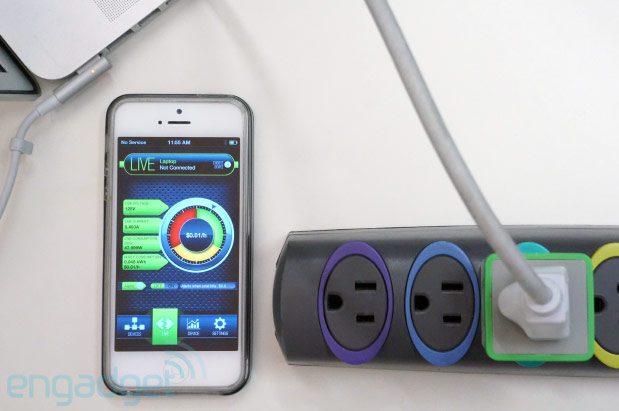
\includegraphics[width=6cm]{existing/meterplug}
    \caption {Meter Plug in the environment}
\end{figure}

\subsubsection{Neurio}

Neurio ~\cite{neurio} is a product that makes monitoring power more accessible.\\ 
Neurio does breakdown data per appliance. It does this by analysing the consumption patterns exhibited by common household devices, matching them to a predetermined pattern, and is then able to determine the difference between an air conditioner, and a refrigerator for example. \\
Unfortunately, the granularity of this product does not allow it to detect all appliances, though it claims to "account for more up to 80\% of the consumption in your home"~\cite{neurio-detection}.\\ Neurio has an open API that allows product developers to take advantage of the energy monitoring technology, and allows for the expansion of control features from the users' smartphone.

Neurio works through attaching a wifi enabled sensor to the main power junction of the household. This sensor then feeds all it's data to the Neurio servers so that it can then be accessed on the users' device.
\begin{figure}[h]
    \centering
    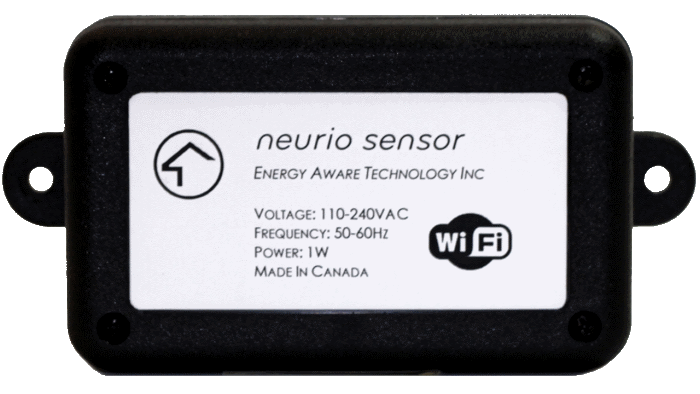
\includegraphics[width=8cm]{existing/neurio-sensor}
    \caption {The sensor used for Neurio}
\end{figure}

\begin{center}
\underline{Pros}
\begin{itemize}
        \item \underline{Easily accessible} - The data supplied by Neurio is easily accessible through smart phones, and the data displayed by the app is easy to understand and digest.
    \item \underline{Minimal} - The Neurio sensor is hidden from view, and is relatively small.
    \item \underline{Reasonably Priced} - Neurio prices up at \pounds55, which is a reasonable price for the ability to look at the overall energy consumption for a household. 
    \item \underline{Customisable} - Neurio is extensible though their development toolkit.
    \item \underline{Realtime Data} - Data is transmitted every split second.
    \item \underline{Customisable} - Neurio can be integrated into IFTT (If then this that) and SmartThings to add additional features, i.e. when the washing machine turns on, you receive a push notification.
\end{itemize}
    
\underline{Cons}
\begin{itemize}
    \item \underline{Granularity} - Neurio can detect only large appliances which according to Neurio make up 80\% of household consumption~\cite{neurioaccuracy}.

\end{itemize}
    
\end{center}

\begin{figure}[H]
    \centering
    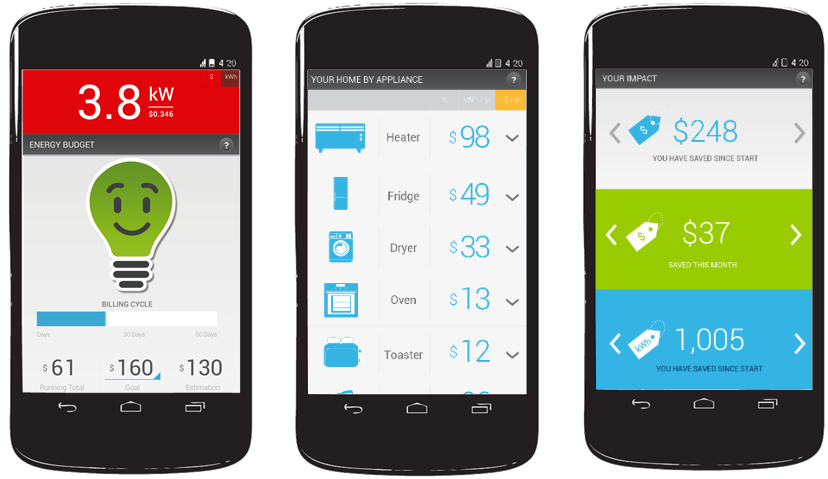
\includegraphics[width=8cm]{existing/neurio-app}
    \caption {The app for the end user.}
\end{figure}


\subsubsection{Kill A Watt}

Kill A Watt ~\cite{killawatt} is a simplistic solution to the energy monitoring issue. It's a very similar to the Meter Plug, without the connectivity. The user knows how much energy an appliance is used through the LCD display immediately above the plug.

\begin{figure}[h]
    \centering
    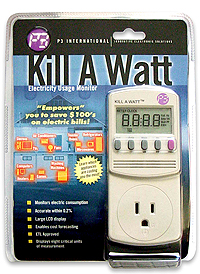
\includegraphics[width=5cm, height=6cm]{existing/killawatt}
    \caption {The Kill A Watt package}
\end{figure}

\begin{center}
    \underline{Pros}
    \begin{itemize}
      \item \underline{Simple} - The Kill A Watt is simple to install and the data it produces is easy to digest.
      \item \underline{Real Time} - The Kill A Watt is always shows the real time energy consumption of the appliance it's connected to.
    \end{itemize}
    
    \underline{Cons}
    
    \begin{itemize}
      \item \underline{Large} - The Kill A Watt is bulky and would stand out in your home environment.
      \item \underline{Expensive} - The Kill A Watt prices up at \pounds20 which is expensive for a device which offers limited functionality.
      \item \underline{Not easily accessible} - In order to view the data, the user will need to be in the vicinity of the plug.
    \end{itemize}
    
\end{center}

\subsection{Related Research}
There is a lot of related work in this field with the aims of aiding a user to be more energy conscious, thereby reducing their energy consumption.\\
This section provides a brief overview of this related work and possible applications to this project.\\[5pt]
The field of power measurement for home appliances is not a new field, it has been around for a long time.\\ As a result, there has been a huge amount of research into different methods of analysing appliances and displaying this data in an easy to understand format for a user to digest.\\
Power signature analysis~\cite{laughman2003power} is a concept whose results can be seen in Neurio, discussed in existing products.\\ 
Laughman and the team theorised that a distributed network of sensors may not be the best way of measuring current of various appliances, especially in large buildings where noise is unpredictable. Instead, they proposed an improvement to nonintrusive load monitoring whereby the harmonic characteristics of appliances were used as an identifier to detect and measure voltage at the electric utility service entry.\\
This concept has been tried and tested, the results showing that the granularity of a system utilising this methodology will only be accurate with a small number of concurrent devices~\cite{liang2010load}.\\
The alternative to the former, is a distributed network of sensors that feedback to a centralised server. In 2008, Bai and Hung investigated the capabilities of a low power embedded system for appliance control and current measurement using Zigbee for communicating data~\cite{bai2008remote}. Their work concluded with a low cost, low power, wireless embedded system that pertained to this architecture.\\
There are a couple of issues with this solution. Firstly, the outlined architecture would not be able to scale to larger buildings. Larger buildings are subject to huge amounts of noise either corrupting packets or blocking them completely. The range of Zigbee would also be a factor in why this solution would not scale favourably, as an extreme example, a 50 storey building would not be a suitable deployment location. Moreover, the final solution was quite bulky, which would be an important factor in many deployment scenarios.\\ 
Rather than using Zigbee for communication, Lien and the team investigated the use of communication over power line~\cite{lien2008power}. Their research lead them to a web based monitor and control platform for their distributed sensors. However, the sensors produced were large and obtrusive in their environment due to the demands and requirements of power line communication. On the other hand, their results were accurate, and integrated extremely well using the inbuilt architecture of the home. \\
Lien and the team also investigated the applications of a remotely controlled outlet system in the household~\cite{lien2006remotely}. This research involved the use of Bluetooth to control appliances, and GSM to send commands to the controller. The downfall of their approach being that the bluetooth modules consumed a lot of power, had a limited range, and were affected by the noise of the environment.\\
The importance of current monitoring is paramount, but it is also important to relay this information to a user in an easy to understand format so that a user can then ammend their behaviour dependant on the information displayed.\\
There have been a number of studies that have investigated the repercussions of energy consumption feedback for users.\\
Costanza in 2012 investigated the importance of Interactive Visualisation in aiding the conservation of energy~\cite{costanza2012understanding}. The paper illustrated that the participants of the study found the engaging nature of the software helped them to identify heavy consumption appliances. In the paper the notion of an activity was introduced, as the participants went about their daily tasks, they were able to associate appliance usage with their activity. \\
A paper was also written on the openness and visibility of energy data, and detailed the methodology of how to design digital technologies to better describe the energy their home is consuming~\cite{price2013looking}. Various different interfaces were trialed and tested, and the results showed that these interfaces benefited households positively and affected their day to day activies.
These papers show that engaging visualisations affect user behavior, and these visualisations could be part of the scope of this project.\\



\subsection{Conclusions}
The selected existing products are from the same area of the market, but each performs the task of energy measurement very differently.\\
The apparent conclusion from the existing products section is there isn't a product on the market that is low cost, low power, discrete in its implementation, accurate and has a per appliance granularity combined with the convenience of accessing data through the use of mobile devices.\\
The related work section highlights areas which a high concentration of research and time has been invested. The research conducted in this field is invaluable, but there are areas where the research is lacking.\\
Laughman's work determined that using the electric utility service entry as a single point of monitoring was an extremely successful approach to the issue at hand. The downsides of the approach being accuracy, as it didn't scale to a large number of devices.\\
Bai's work investigated the use of a network of sensors reporting to a centralised hub, to produce monitoring data for a large number of appliances. This architecture would scale really well if the range of the Zigbee's was unaffected by noise.\\
Lien investigated the possible applications of Bluetooth with a similar architecture to that of Bai's. However, Bluetooth was shown to be too short range and consumed a comparatively large amount of power.\\
Lien also investigated the use of the homes internal architecture, the power line. The work produced a distributed network of sensors that fed back to a centralised point on the power line. There were a couple of drawbacks to this approach, the most important drawback being the size of the sensors.\\
The overall conclusion to be drawn from this selection of papers is that the correct architecture to a successful system is a distributed network of sensors with a centralised point of contact for the sensors.\\
In these papers, power line, Zigbee and Bluetooth communication have been covered extensively. However, there is an important, less traditional medium of communication that has been overlooked, the Earth line. This medium will be one of the main focuses of this project.\\
The final two papers covered in the related work section detailed the importance of visualising the data gathered by the sensors. Therefore data visualisation will be another key aspect of this project.
\subsubsection{Top Level Requirements}

Through the analysis provided in the previous section, there are a number of requirements that can be generated:

\begin{itemize}
  \item \underline{Small} - The device needs to be small and unobtrusive and if possible, it should be hidden.
  \item \underline{Minimalist}- The devices design should be simple and not overly complex.
  \item \underline{Low power} - The device shouldn't consume a lot of energy, as that would defeat the aim of the device.
  \item \underline{Low cost} - The device should be inexpensive, so that the technology is easily accessible to all.
  \item \underline{Simple to install and use} - The device should work "out of the box" and require minimal setup and installation.
  \item \underline{Accessible data}  - The data produced should be instantly accessible through either a web interface or smartphone app.
  \item \underline{Real time} - The data produced and displayed should be real time and up to date.
  \item \underline{Breaks down data per appliance} - The data produced should be tied to a particular appliance so that the user can visually identify each device.
  \item \underline{Reliable} - The device should be reliable and require minimal maintenance.
\end{itemize}

\clearpage
\section{Background}
\subsection{System Outline}
\begin{figure}[H]
    \centering
    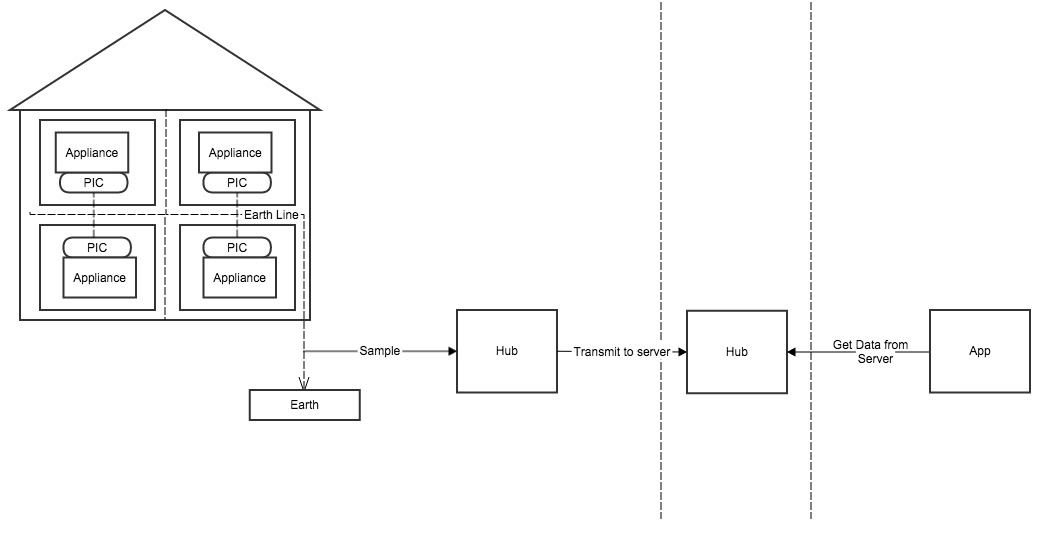
\includegraphics[width=\columnwidth]{diagrams/overalldescript}
    \caption {The proposed system.}
\end{figure}
\subsection{Fuse}
\subsubsection{Hardware Selection}
Based on the requirements, an embedded system seems to be the most applicable technology to this aspect of the project\\
Todays market consists of a large number of embedded devices built for a huge range of tasks.\\
This section will determine the best hardware for the monitoring of appliances.
\paragraph{PIC10F322}
The 10F322~\cite{10f322} is a small surface mount PIC. Counter to the 16f1788, the 10F322 is smaller, far cheaper only costing 56 pence for amounts over 100.
The 10f322 also draws far less power around \SI{0.8}{\micro\ampere} at 32khz.\\
The downsides to using this pic would be that it has no on board serial module. This would increase development time, which may skew other factors of the project.\\
However this PIC would be more suited to a production environment because of its size and price.
%pros
% small
% cheaper 100+ 0.56p
% on board adc
%draws 0.8 microA @ 32 kHz, 1.8V, typical
%cons
% factory flash - unsuitable for development
% no on board serial

\paragraph{PIC16F1788}
The 16F1788~\cite{16f1788} is a large surface mount PIC. The 16F1788 has lots of program memory, RAM  and carries a lot of on board components including an ADC, and Serial I/O. This makes it great for testing and experimenting with new circuits.\\
Conversely, this PIC has a large number of on board components, which increases the price (\pounds1.91),  and the size of the PIC.\\
The power draw of the circuitry is around \SI{8}{\micro\ampere} at 32khz, which would be quite high for a final product.


%pros
% great for testing large amount of ram and program memory
% on board serial
% on board adc
% debug enabled
%cons
% big
% draws 8 microA @ 32 kHz, 1.8V, typical
% pricey 100+ 1.91 




\subsubsection{Conclusions}
The 16f1788 would be the ideal PIC for testing and developing the circuitry for the Fuse. However, when entering production, the 10f322 would be the PIC of choice due to its size, price and selection of components.



\subsection{Hub}
\subsubsection{Hardware Selection}
The requirements dictate that something more powerful than a traditional embedded system will need to be used to process and store the data generated by the Fuses.\\
The hardware will need to be able to have either wired or wireless Internet connectivity, as well as being low cost, low power and able to process quite a lot of data.\\
Over recent years, a lot of money has been used to create affordable, small, powerful computers that are widely available.\\
This section will compare key players in this market to determine the hardware that will be utilised in this project.
\paragraph{Raspberry Pi}
The Raspberry Pi~\cite{raspberrypi} is the most well known member of this market, and with the most recent introduction of the Raspberry Pi 2, is a strong market leader as well.\\
The Raspberry Pi has a number of hardware components that can be controlled by a user, including a Serial I/O port. This Serial I/O port can be used to communicate with external embedded systems, which could be useful for the project.\\
The Raspberry Pi costs around \pounds30 depending on the model. It comes with Ethernet as standard, but external modules can be added to introduce other technologies such as WiFi and Bluetooth. This will obviously incur additional costs.\\
The power consumed by the Pi on average is around \SI{700}{\milli\ampere} which is really low for such a powerful computer.


\paragraph{Hummingboard}
The Hummingboard~\cite{hummingboard} is a relatively new player in the market.\\
It's more expensive (\pounds15 more) than the Raspberry Pi, but offers more RAM, and a faster processor.\\
Like the Raspberry Pi, it offers GPIO and UART built in. Ethernet is also offered as standard, but again like the Raspberry Pi, for an additional amount, WiFi and Bluetooth can be added.\\
The operating system is based off linux, so it has support for quite a lot of the standard linux distributions, much like the Raspberry Pi.\\
The Hummingboard slightly consumes more power than the Raspberry Pi, approximately \SI{780}{\milli\ampere} in total, but this would make a negligible difference overall.
\paragraph{Beaglebone Black}
The Beagle Bone~\cite{beaglebone} prices \pounds5 above the Raspberry Pi and offers a 1gHz processor instead of the Pi's 700 mHz one.\\
It doesn't have inbuilt UART for serial communications, but it does have a large number of GPIO pins.\\
The power consumed by the Beaglebone is half that of the Raspberry Pi, with \SI{350}{\milli\ampere}. However it is missing components that the Raspberry Pi does have.

\subsubsection{Conclusions}
It appears that the best candidate for the hub element of this project is the Raspberry Pi.\\
It is the cheapest, and offers a wide range of features as well consuming a small amount of energy. The measurements taken were from the original Model B, and at the time of writing, the Raspberry Pi 2 has just been released, offering improved features for the same price.





\subsection{App}
\subsubsection{Frameworks}
In the previous section, the MEAN stack was chosen as the preferable stack. The element applicable to client-side applications in the MEAN stack is Angular.\\
As previously mentioned Angular~\cite{angular} uses the MVC model to control and display data to a user. Traditionally, Angular is only used in web applications, more recently however, Web Frameworks are moving into the cross platform world.

\paragraph{Ionic}
Ionic~\cite{ionic} is a framework created by 'Drifty', and is powered by Angular JS, conforming to the MEAN stack requirement.\\
It is a high performance, native focused, beautifully designed, cross platform framework allowing for rapid yet stable development.\\
Currently, the cross platform element supports only iOS and Android, but Windows phone and FirefoxOS are coming soon.\\
Ionic utilises Angular lending itself to the MVC architecture, which allows the compartmentalisation of the app.\\
Like many mobile frameworks, it has a vast amount of built in components, to make the final app look and feel native to the platform.\\ PhoneGap~\cite{phonegap} and Cordova~\cite{Cordova} are used to wrap the HTML, CSS and JavaScript produced by Ionic and hosts them using native binaries.

\paragraph{Ratchet}
Ratchet~\cite{ratchet} was developed by Connor Sears who worked at twitter and need a way of rapidly prototyping new UI ideas for the native Twitter app.\\
Unlike Ionic, this framework doesn't use Angular, and uses native javascript to perform UI interactions.\\
This may make app development worse due to the lack of compartmentalisation, and as the project scales, source code will be harder to maintain and update.\\
Ratchet also has a number of built in UI components, however it seems like Ratchet doesn't make any effort to appear native to the platform.\\
It also doesn't adhere to the MEAN stack as it doesn't intertwine with Angular, and it seems like this framework is more focused on prototyping than on formal app development.

\paragraph{Famo.us}
Famo.us~\cite{famous} is an extremely new framework, and is in very early stages of Beta, the current version being 0.3 at the time of writing.\\
This framework can easily be integrated with Angular, matching the MEAN stack requirement.\\
This framework claims to be a platform for building high-performance user interfaces that can be used to display complex animations and has an inbuilt physics engine to support games development.\\
Although this framework simplifies UI development, it doesn't simplify the overall app development like the Ionic framework does.\\
It's also in early development, and appears to not offer as many features as Ionic or Ratchet.

\subsubsection{Conclusions}
The framework that meets the most requirements appears to be the Ionic Framework.\\
It offers great performance, a huge range of UI tools, Angular at it's core and cross platform support.\\
It has a great support community behind it, and it is well established in the development world.\\
These combined factors make it in obvious choice for the basis of the application for the project.




\subsection{Server}

\subsubsection{Web Server}
There are a number of web server packages out there, the most popular being Apache.\\
Apache has been around for a long time, and the most common stack for an Apache server is LAMP: Linux, Apache, MySQL and PHP.\\
Considering that the system will be receiving a large amount of data, will be used in conjunction with a cross platform app and the system will be event driven, the aforementioned Apache LAMP stack may not necessarily be the best choice.\\
There are many modern variations and implementations of web servers around today, developers no longer need to transition between different languages. Python developers can transition to Django, a Python web server. They can build apps using python, transition to the server side development environment, and build the API. The story is the same with Ruby, Perl and more recently, JavaScript.\\
\paragraph{MEAN Stack}
The MEAN~\cite{mean} stack is built from four components: MongoDB - the database, Express - the web application framework, Angular - the Client side framework and finally Node to create the MEAN stack.\\
MongoDB is a NoSQL database and will be discussed later on in this document, when determining the correct database software.\\
Express~\cite{express}~\cite{whatisexpress} is a Web Application framework which manages the routing for the application, as well as simplifying the overall process getting request data. It acts as the glue between Node, and MongoDb.\\
Angular is a language built by Google, based on Javascript. It implements the MVC architecture, and is implemented client side, using HTTP requests or local storage for data.\\
Node.js~\cite{nodejs} is an open source runtine environment for server side applications, and provides an event driven architecture and non blocking I/O making it extremely scalable.\\
Node replaces the Apache element of the LAMP stack, and uses the Google V8 JavaScript engine~\cite{v8engine} used in Google's popular Chrome browser. The v8 engine compiles and executes JavaScript, rather than the more traditional model of interpretation on the fly.\\
When comparing Node to the traditional Apache LAMP stack~\cite{phpvsnodejs}~\cite{nodejsvsapache} there are immense speed improvements due to the non-blocking nature of Node. This is extremely important for a number of reasons:
\begin{itemize}
  \item \underline{Scalable} - Node works concurrently, the number of users makes no difference to the page load time, improving the aspect of scalability.
  \item \underline{Lower Costs}- Nodes concurrency removes the issue of concurrent users impacting load times, this means that less physical resources will be required.
  \item \underline{Fast} - As Node is concurrent, pages load lightning quick, improving the experience for the end user.
\end{itemize}

\paragraph{Django}
Django~\cite{django}, unlike Node.js, can be configured to be layered upon a number of base web servers, and is a Web Framework.\\
In the traditional LAMP model, Django takes the place of PHP, and instead uses Python to construct the application.\\
As PHP is a language, it can only be compared to Python in this case. The performance of Python~\cite{djangovsphp} is 2-3 times faster than PHP, but also used 2 times as much memory. So there is a trade off between performance and server resources which would be important when scaling the solution.

\paragraph{Ruby on Rails}
Ruby on Rails~\cite{ruby} is similar to Django, it is a web framework, and it acts as a replacement for the PHP element of the LAMP stack.\\
As PHP is a language, it can only be compared to Ruby in this case. The performance of Ruby~\cite{rubyvsphp} is 2-4 times faster than PHP, but again uses more memory, and thusly there is yet again a trade off between performance and server resources, affecting scalability.


\subsubsection{Database}
The database is an important consideration in any project. In the previous section, it was determined that a solution involving MEAN stack was preferable over the more traditional LAMP stack solution.\\
The database layer is separate, but at the same time is intertwined with the server layer. This means that there needs to be a relatively easy way of communicating between the two layers.\\
This section will compare various database solutions applicable to the kind of project discussed in this document: the Internet of things.\\

\paragraph{MongoDB}
MongoDB~\cite{mongodb} harnesses the benefits of a NoSQL database, but at the same time retains the relational aspects of SQL.\\
Documents are stored using JSON documents, and B-Trees are used for quick look up times.MongoDB also scales across a number of servers using Passive server replication.\\
It's best used for real time systems, with rapidly changing data~\cite{databasecomparison}, which is directly applicable to the project.\\
It's also worth considering that the rest of the stack uses the *EAN model. Thus the majority of development will be in Javascript, implying that it might be best to store objects in JSON for easy storage and retrieval. MongoDB's main storage format is JSON, it will therefore be easy to integrate with the rest of the stack. 

\paragraph{Redis}
Redis~\cite{redis} is an advanced key-value cache and store. It stores data in traditional data structures, like Strings, Hashes and many more.\\
Redis stores all objects in memory, which may make it unsuitable for the project in the long term. A user can however partition memory across server machines~\cite{redisfaq}, so that Redis can expand beyond the limits of a single machines.\\
The issue with redis is that there isn't a direct translation between database and server like there is in MongoDB, which may make storage and retrieval difficult. It is also far easier to increase disk space than it is RAM.\\
Redis is best used for projects with rapidly changing data with a foreseeable database size~\cite{databasecomparison}. In this project, the database size is not fully predictable due to a number of variables, like the number of Fuses and the number of Hubs a user may own.

\paragraph{CouchDB}
CouchDB~\cite{couchdb} is written in Erlang, and stores data in JSON format. CouchDB uses HTTP requests to perform CRUD (Create, Read, Update, Delete) operations on the data. 
%MIGHT NOT NEED THIS CRAP...
%------------
The interesting concept behind this is that CouchDB can actually act as the applet, and allows easy content management using a control panel integrated into the database.\\
%------------
CouchDB unfortunately doesn't offer dynamic queries, instead offering map/reduce functions. It's also not relational, both of which will impact performance in the long term.\\
CouchDB is best used for accumulating occasionally changing data, where queries have to be predefined~\cite{databasecomparison}. In the project, data is dynamic and constantly changing, CouchDB is not. This factor, in combination with the non-relational nature of CouchDB, renders it unusable in this project.

\subsubsection{Conclusions}
The MEAN stack seems to be the obvious conclusion from the comparison above. Scalability and performance are key factors in this decision. As the system becomes more widely used, more requests will be received. A stack like the MEAN stack where the number of requests makes little or no impact is ideal.\\
Development time is also another key factor. Using the MEAN stack will result in faster development, and it will be easy to integrate the resulting API into Angular for a cross platform app, rather than two entirely separate native apps for Android and iOS.



\clearpage
 %--------------------------
 %DESIGN
 %--------------------------

\section{Design \& Implementation}
\subsection{Use Case Diagram}
\begin{figure}[H]
    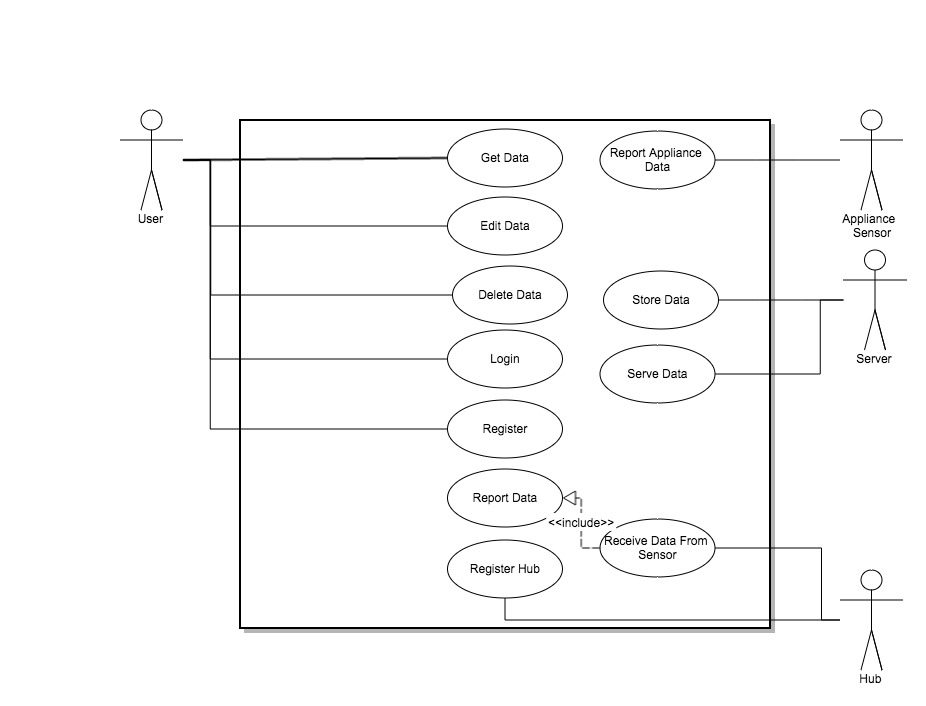
\includegraphics[width=\columnwidth]{diagrams/UseCase}
    \caption {Use Case Diagram}
    \label{fig:usecaseoverall}
\end{figure}
Figure~\ref{fig:usecaseoverall} shows the use case diagram for the system.\\
A \textbf{User} can perform various actions, they can get, edit and delete data, and they can also login and register.\\
A \textbf{Fuse} can only report appliance data, and transmit it over the Earth line.\\
A \textbf{Hub} can receive data from a \textbf{Fuse}, report data and also register with the \textbf{Server}.\\
The Server can store and serve the data stored in the database.

\subsection{Overall System Architecture}
\begin{figure}[H]
    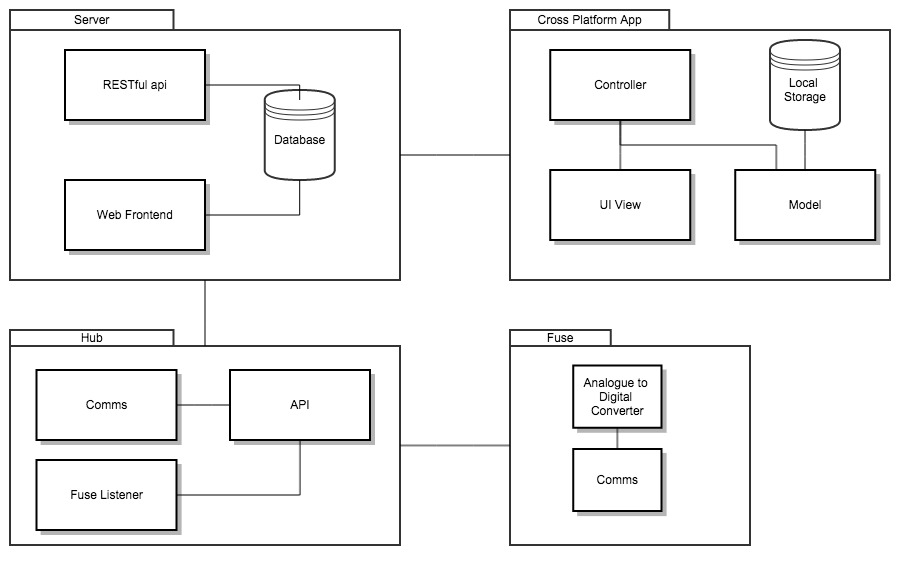
\includegraphics[width=\columnwidth]{diagrams/Architecture}
    \caption {Overall System Architecture}
    \label{fig:systemarchoverall}
\end{figure}

Figure~\ref{fig:systemarchoverall}


 %--------------------------
 %Implementation
 %--------------------------






\subsection{Fuse}
The Fuse consists of a PIC16f1788 running custom assembly software. The schematics of the circuit, and the overall software architecture of the Fuse are described in this section.

\subsubsection{Requirements}
\begin{itemize}
\item \underline{Transmit Data} - The Fuse should transmit data using the Earthed line.
\item \underline{Accurate} - The Fuse should be accurate with its samples.
\item \underline{Small} - The Fuse should be small.
\item \underline{Low Cost} - The Fuse should be low cost.
\item \underline{Low Power} - The Fuse should not consume a large amount of power.
\end{itemize}

\subsubsection{Architecture Diagram}

\begin{figure}[H]
    \centering
    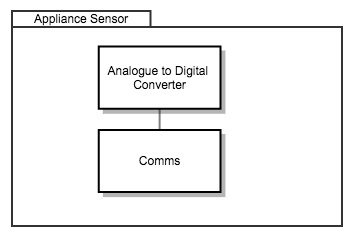
\includegraphics[width=8cm]{diagrams/fuse}
    \caption {Fuse Architecture Diagram}
\end{figure}
\subsubsection{Schematics}
\begin{figure}[H]
    \centering
    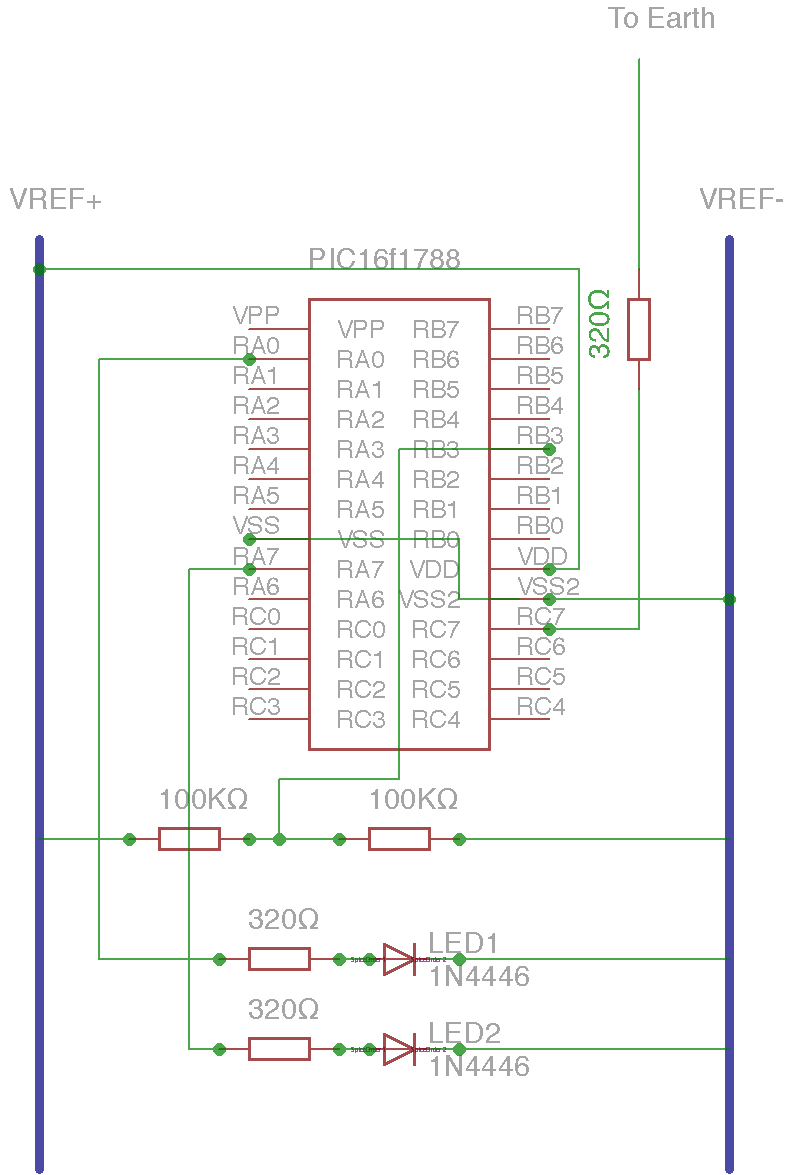
\includegraphics[width=8cm]{/schematics/fuse}
    \caption{The schematic for the fuse.}
    \label{fig:fuseschematic}
\end{figure}
Figure~\ref{fig:fuseschematic} shows the schematic for the current implementation of the fuse.\\
Currently the input for the fuse is a voltage divider using two 100K resistors across VREF+, which is then connected to RB3, the input for the ADC.\\
There are two status LEDs. LED1 shows the on state of the fuse, when the fuse transmits LED2 will light up for the duration of transmission.\\
The fuse transmits using pin RC7 to a faux Earth line connected to the hub. This line is protected using a 320 ohm resistor.


\subsubsection{Software}
The software for the Fuse is written in assembly.\\
Assembly is used for extremely low level embedded devices. The reason assembly has been chosen is because it offers a level of accuracy that is extremely hard to achieve through using a higher level language like C.\\

\paragraph{Average Over Time}
The Fuse generates data that can be used to generate an average over time.\\
When a sample is collected by the ADC, the sample count is incremented and the ADC result is added to a sum.\\
When the fuse transmits, the packet contains the sample count and the sum of all of the samples currently held in memory. The average voltage is then calculated on the Hub, and sent to the server.

\paragraph{Extended Hamming Code}
To provide robust transmission down a usually noisy line, there needs to be a form of error correction in place.\\
The chosen form of error correction is Extended Hamming Code, due to it's extensive use throughout the industry.\\
Each byte will be encoded before transmission in a 4:8 encoding ratio. This means every 4 bits will produce a byte when encoded.\\
Unfortunately, this does produce more bytes, which is the downfall of this encoding, however it will make the transmission more robust and more impervious to errors.\\
In Extending Hamming Code, each nibble is encoded using a look up table:

\begin{table}[H]
\centering
\resizebox{4cm}{!} {%
    \centering
    \begin{tabular}{| l | l |}
    \hline
    Hex Value & Encoded Result  \\ \hline
    0 & 0x15 \\ \hline
    1 & 0x02 \\ \hline
    2 & 0x49 \\ \hline
    3 & 0x5e \\ \hline
    4 & 0x64 \\ \hline
    5 & 0x73 \\ \hline
    6 & 0x38 \\ \hline
    7 & 0x2F \\ \hline
    8 & 0xD0 \\ \hline
    9 & 0xC7 \\ \hline
    A & 0x8C \\ \hline
    B & 0x9B \\ \hline
    C & 0xA1 \\ \hline
    D & 0xB6 \\ \hline
    E & 0xFD \\ \hline
    F & 0xEA \\ \hline
    \end{tabular}
}
\caption{Hamming code translations}
\end{table}
Once the nibble is encoded, the byte is transmitted using RS232. Hamming encoding will be discussed again later on in this document, with a further explanation of how it works.

\paragraph{Random Transmission}
The timings between each transmission is 'random'. This randomness is generated through the incrementation of a variable throughout various points in the code. When this variable hits a specific value, data will then be transmitted. \\
The reason for random transmission is to reduce collisions on the line. The hope is that through using a randomised variable, fuses will transmit at different times.

\paragraph{Packet Structure}
The following details the packet structure that is transmitted by the Fuse.\\
The packet consumes 7 bytes. Due to hamming code, this packet size is doubled, making the final packet size 14 bytes.\\[5pt]
\begin{table}[H]
\centering
\resizebox{8cm}{!} {%
    \centering
    \begin{tabular}{| l | l | p{2cm} |}
    \hline
    Label & Bits &  Address \\ \hline
    Device ID Lower & 8 & 0x26\\ \hline
    Device ID Higher & 4 & 0x27\\ \hline
    Sample Count Lower & 4 & 0x27\\ \hline
    Sample Count Higher & 8 & 0x28\\ \hline
    Total Lower & 8 & 0x29\\ \hline
    Total Middle & 8 & 0x2A\\ \hline
    Total Higher & 8 & 0x2B\\ \hline
    Checksum & 8 & 0x2C\\ \hline
    \end{tabular}
}
\caption{The break down of the packet}
\label{tab:packet}
\end{table}
\underline{Packet Description}
\begin{itemize}
\item \underline{Device ID} - The Fuse's ID generated at the factory. It can have a value anywhere between 0 and 4095.
\item \underline{Sample Count} - This variable is incremented each time a sample is taken, and allows the hub to work out the average voltage consumed by the connected appliance. The maximum value being 4095.
\item \underline{Total} - This variable is the result of the summing of ADC values after a new sample is taken. It allows the hub to work out the average voltage consumed by the connected appliance. The maximum value for these 24 bits is 16,777,216.
\item \underline{Checksum} - Before the packet is transmitted, each register is added to the checksum register, ignoring overflow. This variable will then be used Hub-side in conjunction with hamming code, to determine if the packet has been received correctly.
\end{itemize}

\paragraph{Sampling}
Sampling will occur very regularly, depending on the final clock rate of the PIC.\\
The PIC will continuously sample the ADC until the random transmission variable is matched.\\
In software, each time a sample is captured, it will be added to the Total Count, which is contained in 3 bytes as detailed in table~\ref{tab:packet}. At the same time, the sample count will also be incremented. \\
When a hub receives the packet, it will be able to determine the average voltage being consumed by that appliance by dividing the total by the number of samples.

\subsubsection{Hardware}
The PIC that is currently in use is the 16F1788. This PIC has simply been chosen for the amount of on board components, and ease of integration between these various components.\\
The PIC itself is far too big for the final product and there therefore should be a contingency strategy in place for the eventuality of moving to a smaller chip like the 10F322.

\paragraph{USART}
The 16F1788 has an on board serial chip. This chip will be used to transmit the packet using the USART standard in serial communications.\\
Depending on the clock rate, the serial communication will occur at different baud rates. This will be a factor for testing in the evaluation section.

\subsection{Hub}
The Hub consists of a Raspberry Pi connected to a custom circuit used to intercept messages from the fuse before they reach Earth. In this section, the additional circuitry is described as well as the software architecture of the Hub.
\subsubsection{Requirements}
\begin{itemize}
\item \underline{Transmit Data} - The Hub should transmit received data to the server.
\item \underline{Receive Data} - The Hub should be able to detect packets being transmitted on the Earthed line.
\item \underline{Small} - The Fuse should be small.
\item \underline{Low Cost} - The Fuse should be low cost.
\item \underline{Low power} - The Fuse should be low power, and not consume large amounts of electricity.
\item \underline{Process Data} - The Hub should be capable of processing data with ease.
\end{itemize}
\subsubsection{Architecture Diagram}
\begin{figure}[H]
    \centering
    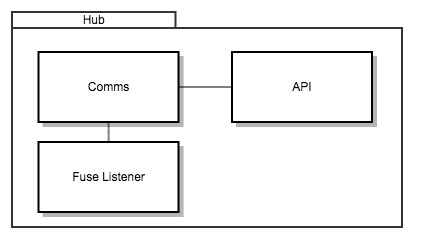
\includegraphics[width=8cm]{diagrams/hub}
    \caption {Hub Architecture Diagram}
\end{figure}
\subsubsection{Schematics}
\begin{figure}[H]
    \centering
    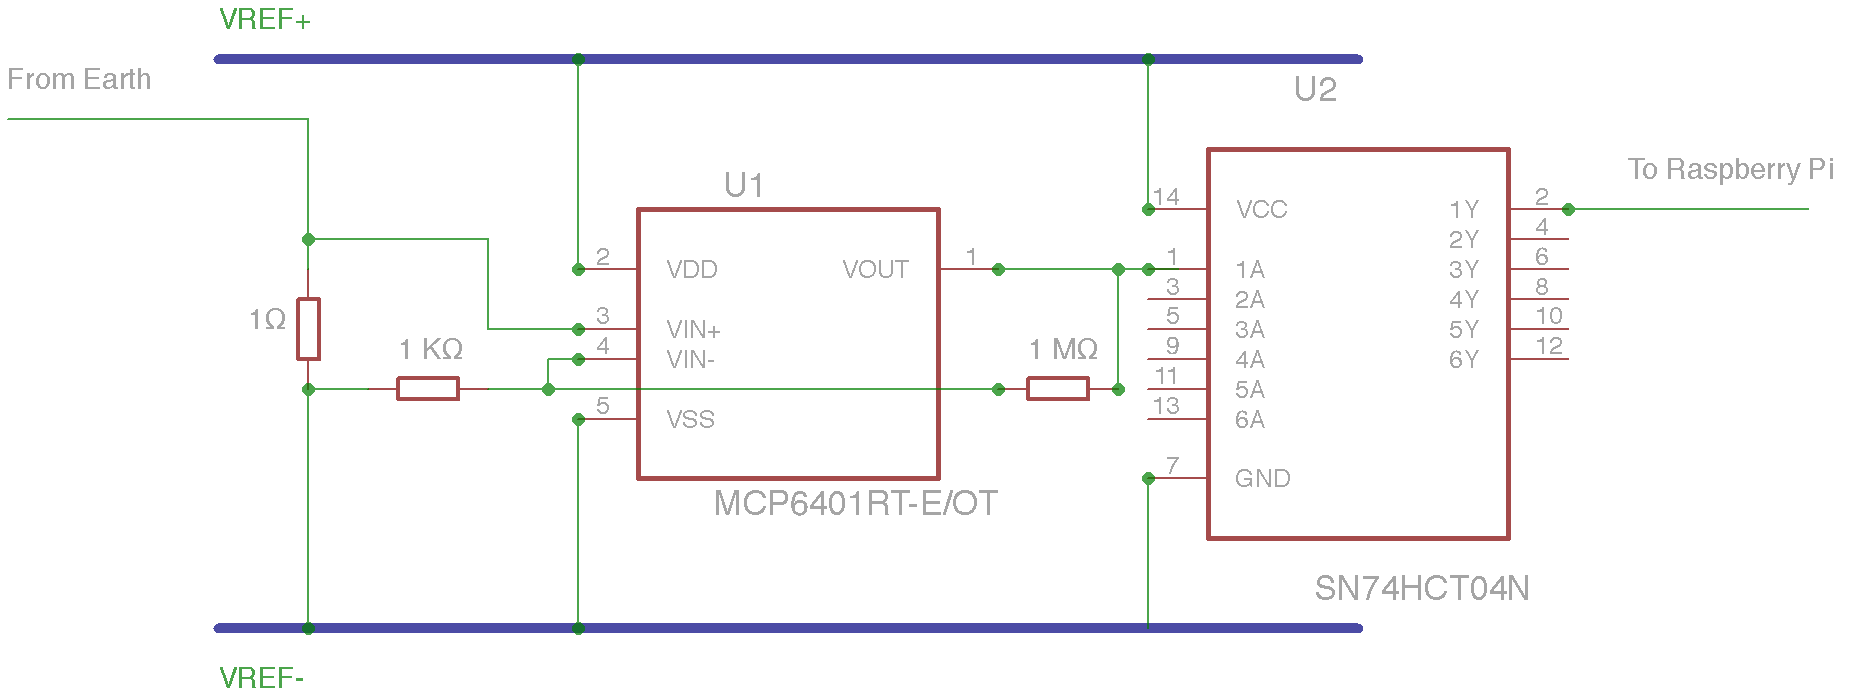
\includegraphics[width=\columnwidth]{/schematics/hub}
    \caption{The schematic for the Hub.}
    \label{fig:hubschematic}
\end{figure}
The additional circuitry in figure~\ref{fig:hubschematic} is used to detect messages sent from the Fuse before they hit actual Earth.\\
A precise OpAmp (MCP6401RT) is used to amplify the packets, the output of which is used in conjunction with a Hex Inverter to transpose the packets from inverted RS232 to non-inverted RS232 to be processed by the Pi.\\
A 1 Ohm resister is used to provide a small difference between VIN+ and VIN- without distorting the signal. The OpAmp then uses a closed loop to determine the level of gain it should apply to the signal, which is calculated by dividing 1 megohm by 1 kilohm  resulting in a gain of 1,000.
\subsubsection{Software}
The software for the Hub is written in Python.\\
Python is a really useful language, especially on the Raspberry Pi, where there are a lot of translations from lower level C to high level python.\\

\paragraph{Class Diagram}
\begin{figure}[H]
    \centering
    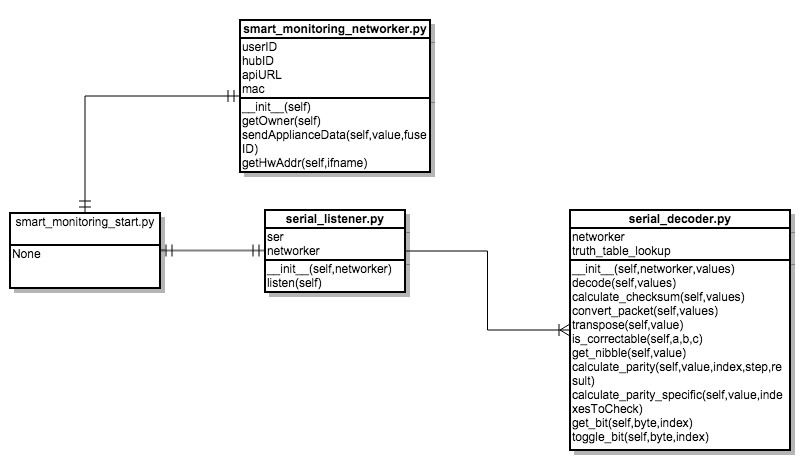
\includegraphics[width=\columnwidth]{/diagrams/hubclassdiagram}
    \caption{The class diagram for the Hub software.}
    \label{fig:hubclassdiagram}
\end{figure}
Figure~\ref{fig:hubclassdiagram} shows the final class diagram for the hub software.\\
Each class is isntantiated using the smart\_fuse\_start.py file. When this file is executed, the smart\_fuse\_networker class is instantiated, and getOwner is called. This prompts the hub to talk to the server and obtain its credentials and also the user account it's linked to. If no user account is linked, the hub will check at regular 30 second intervals until a user account has been found.\\
Once the hub has obtained all of the required details, the serial\_listener class is instantiated with the instance of networker previously instantiated. The listen function is called on the serial listener, which will listen forever. This is the main loop for the program.\\
When the serial\_listener class successfully receives a full packet, it passes the packet and an instance of networker to the serial\_decoder and begins execution in a separate thread. If the serial\_decoder successfully decodes the packet, it is transmitted to the server using the sendFuseData function of the networker class passed in by the serial\_listener.
\paragraph{Event Driven Architecture}

\begin{figure}[H]
    \centering
    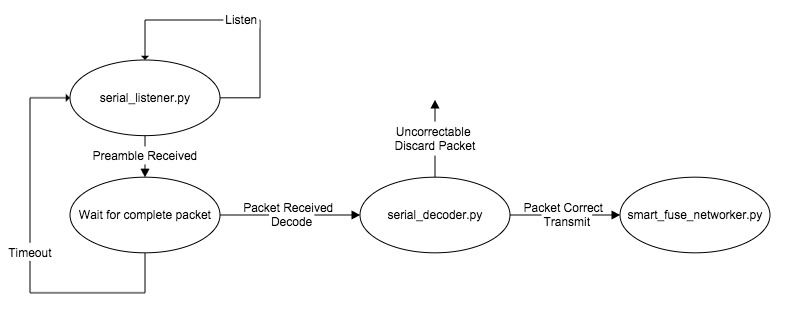
\includegraphics[width=\columnwidth]{/diagrams/eventdriven}
    \caption{The event driven architecture for the Hub.}
    \label{fig:eventdriven}
\end{figure}

Figure~\ref{fig:eventdriven} shows the event driven architecture used by the Hub.\\
The serial listener listens for the preamble which is 0x55. When It successfully receives the preamble, it listens for the next 14 consecutive bytes, if there is more than a millisecond gap between bytes, the whole packet is discarded, and the listener is reset.\\
If the listener receives all 14 bytes, it then starts up a Python Process to handle the decoding and transmission of the received data. Once the process has started, the listener immediately resumes listening for incoming data.\\ 
The serial decoder operates in a separate thread (or Process) and as the name suggests, decodes the packet using Extended Hamming Code. If the packet is deemed correct, the data is sent to the server and the Process terminates. If the packet is uncorrectable, the packet is discarded and the Process terminates.

\paragraph{Extended Hamming Code}
As the Fuse is using Extended Hamming Code to communicate, the Hub must be able to decode the messages received.\\
Extended Hamming Code allows the receiver to determine the number of incorrect bits, and also the location of the incorrect bits. If the number of incorrect bits is one, then the receiver is able to correct this value, and proceed with processing the packet.\\
Unfortunately if there is more than one error, the packet is unable to be corrected, and therefore must be discarded.\\
On top of hamming code, there is a check sum. So even if the hamming code check succeeds, there is another layer of checking before the packet is determined to be valid.\\[5pt]
\underline{Extended Hamming Code Example:}\\[5pt]
Say the following byte is received:
\begin{table}[H]
\centering
\begin{tabular}{| l | l | l | l | l | l | l | l | l |}
\hline
b7 & b6 & b5 & b4 & b3 & b2 & b1 & b0 & Hex\\ \hline
1 & 1 & 1 & 1 & 1 & 1 & 1 & 1 & 0xFF\\ \hline
\end{tabular}
\caption{An incorrect byte received by the hub.}
\label{tab:incorrectpacket}
\end{table}

However the byte transmitted from the fuse was the following:
\begin{table}[H]
\centering
\begin{tabular}{| l | l | l | l | l | l | l | l | l |}
\hline
b7 & b6 & b5 & b4 & b3 & b2 & b1 & b0 & Hex\\ \hline
1 & 1 & 1 & 1 & 1 & 1 & 0 & 1  & 0xFD\\ \hline
\end{tabular}
\caption{The actual byte sent by the hub.}
\label{tab:correctpacket}
\end{table}

The hub would go through the following process to determine if the byte requires correction:\\
\begin{figure}[H]
\centering
overall parity = b7 \^{} b6 \^{} b5 \^{} b4 \^{} b3 \^{} b2 \^{} b1 \^{} b0\\
check 0 = b7 \^{} b5 \^{} b1 \^{} b0\\
check 1 = b7 \^{} b3 \^{} b2 \^{} b1\\
check 2 = b5 \^{} b4 \^{} b3 \^{} b1\\
\caption{The XOR calculations used in Extended Hamming Code~\cite{extendedhamming}}
\label{fig:xorcalcs}
\end{figure}

If the overall parity variable is 1, 0 or 2 errors occurred. If checks 0-2 are equal to one, then the byte was received intact, otherwise it was damaged beyond repair.\\
If the overall parity variable is zero it means that there is a single bit error that can be corrected.\\
The following look up table can be used to identify the incorrect bit:
\begin{table}[H]
\centering
\begin{tabular}{| l | l | l | l |}
\hline
Check 0 & Check 1 & Check 2 & Meaning\\ \hline
1 & 1 & 1 &´error in bit b6\\ \hline
1 & 1 & 0 & error in bit b4\\ \hline
1 & 0 & 1 & error in bit b2\\ \hline
0 & 1 & 1 & error in bit b0\\ \hline
0 & 0 & 1 & error in bit b7\\ \hline
0 & 1 & 0 & error in bit b5\\ \hline
1 & 0 & 0 & error in bit b3\\ \hline
0 & 0 & 0 & error in bit b1\\ \hline
\end{tabular}
\caption{The look up table used in Extended Hamming Code to identify incorrect bits~\cite{extendedhamming}}
\label{tab:paritylookup}
\end{table}

Using the example of the incorrect byte in table~\ref{tab:incorrectpacket}, the checks can be evaluated:
\begin{figure}[H]
\centering
overall parity = 1 \^{} 1 \^{} 1 \^{} 1 \^{} 1 \^{} 1 \^{} 1 \^{} 1 = 0\\
check 0 = 1 \^{} 1 \^{} 1 \^{} 1 = 0\\
check 1 = 1 \^{} 1 \^{} 1 \^{} 1 = 0\\
check 2 = 1 \^{} 1 \^{} 1 \^{} 1 = 0\\
\caption{Attempting to correct the incorrect packet}
\label{fig:xorexample}
\end{figure}
Figure~\ref{fig:xorexample} shows the resulting values from processing the incorrect byte from table~\ref{tab:incorrectpacket}.\\
The overall parity check indicates that there is a one bit correctable error. Then the checks 0-2 are calculated and subsequently used in the lookup table~\ref{tab:paritylookup}. The lookup table indicates that bit one is incorrect, bit one is flipped, and the corrected byte is:
\begin{table}[H]
\centering
\begin{tabular}{| l | l | l | l | l | l | l | l | l |}
\hline
b7 & b6 & b5 & b4 & b3 & b2 & b1 & b0 & Hex\\ \hline
1 & 1 & 1 & 1 & 1 & 1 & 0 & 1  & 0xFD\\ \hline
\end{tabular}
\caption{The corrected byte.}
\label{tab:correctedbyte}
\end{table}

\subsection{App}
\subsubsection{Requirements}
\begin{itemize}
\item \underline{Cross Platform} - The application should be Cross Platform to allow for rapid development.
\item \underline{Usability} - The application should maintain similar UI components to that of native apps, and should be easy to use.
\item \underline{Performance} - The performance of the application should be fast, and shouldn't be greatly affected by large datasets.
\item \underline{Integrate into the MEAN stack} - The application should display integrate into the MEAN stack with ease.
\item \underline{Real Time} - The application should display user information in real time.
\item \underline{Consistent} - The application should have a consistent state over different platforms.
\item \underline{Visualisation} - The application should provide a good visualisation of data held on the server.
\end{itemize}
\subsubsection{Architecture Diagram}
\begin{figure}[H]
    \centering
    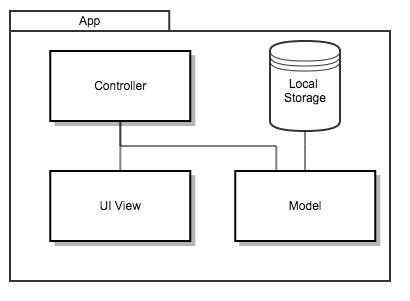
\includegraphics[width=8cm]{diagrams/app}
    \caption {Application Architecture Diagram}
\end{figure}

\subsubsection{MVC}
Angular lends itself to the MVC~\cite{mvc} architecture. This means that the different elements of an application are divided into 3 distinct sections. The Model translates to application data, the view is what the user sees and the controller is what the user interacts with.\\

A visualisation of this can be seen below in Figure 15:
\begin{figure}[H]
    \centering
    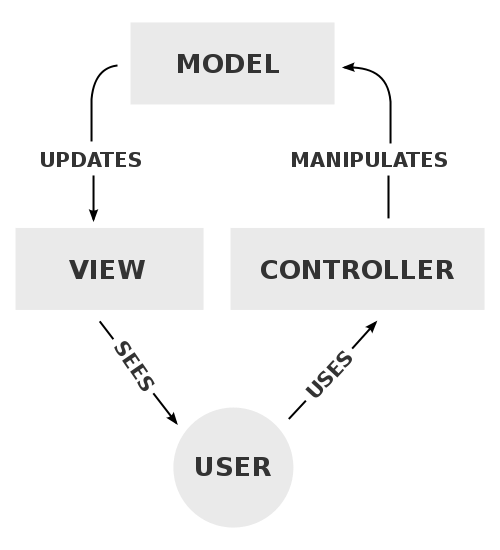
\includegraphics[width=8cm]{/diagrams/mvc}
    \caption {The model view controller architecture.~\cite{mvcimage}}
\end{figure}

\paragraph{Folder Structure}
The main benefit of MVC is a tidy folder structure with a high level of compartmentalisation for the code base as seen in Figure 16:

\begin{figure}[H]
    \centering
    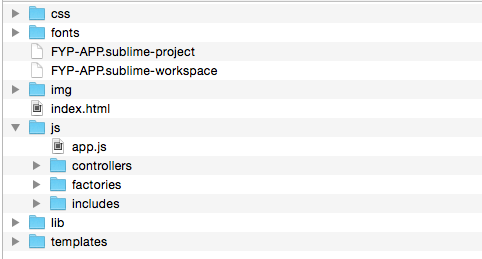
\includegraphics[width=8cm]{/misc/folders}
    \caption {The folder structure for the application.}
\end{figure}
The views are contained in templates, the controllers are in the controllers folder and the models are contained within the factories folder.\\

\subsubsection{Storage}
There is a caching model in place for the application. When a controller is loaded, it asks the model to retrieve local data for the current day. If the model has data for the current data, the view will be updated. Otherwise, the model will fetch fresh data from the api.\\
Every single view implements a way of refreshing the data stored on the device. In the application a user can do this by pulling down on the view, triggering a controller event which forces the application to ask for fresh data from the server. The cached data is also updated when the data is returned from the API.

\begin{figure}[H]
    \centering
    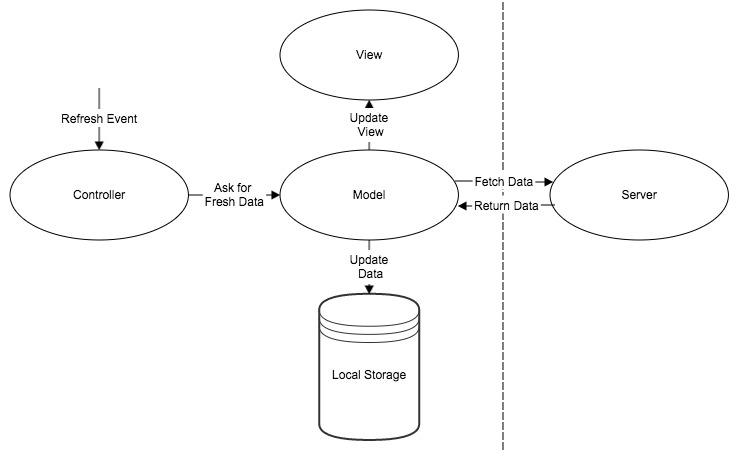
\includegraphics[width=\columnwidth]{/diagrams/mvcrefresh}
    \caption {A diagram of the refresh event}
\end{figure}

\subsubsection{User Interface}
In this section, each view will be described. The thought behind each views' design and the UI features will also be discussed
\paragraph{Icon, splash and login}
\begin{figure}[H]
    \centering
    \begin{subfigure}[t]{0.32\columnwidth}
        \centering
        \frame{
\includegraphics[width=\columnwidth]{/screenshots/insitue}}
        \caption{The application icon}
    \end{subfigure}
    \begin{subfigure}[t]{0.32\columnwidth}
        \centering
        \frame{
\includegraphics[width=\columnwidth]{/screenshots/splash}}
        \caption{The application splash view}
    \end{subfigure}
    \begin{subfigure}[t]{0.32\columnwidth}
        \centering
        \frame{\includegraphics[width=\columnwidth]{/screenshots/login}}
        \caption{The application login view.}
    \end{subfigure}
    \caption{The application icon, splash and login views}
    \label{fig:iconsplashlogin}
\end{figure}
In figure~\ref{fig:iconsplashlogin}.a, the application icon is shown in situ on an iOS device. The icon is on the second to last row, second in from the left.\\
The icon uses the university colour scheme which persists throughout the entire application. The icon is also reused as a menu option in the hamburger menu.\\
Figure~\ref{fig:iconsplashlogin}.b shows the splash view which is presented every time the application is freshly opened, giving time for resources to be loaded in the background.\\
The final figure~\ref{fig:iconsplashlogin}.c shows the view that is presented when the user has no local session stored on the device. If a user has logged into the application at a previous point, their user profile is stored locally and this view is skipped, allowing the seamless resuming of a previous session.\\
If the login button is clicked, a login form is presented, similarly, if the register option is pressed a registration form is presented to the user.

\paragraph{Home and Menu}
\begin{figure}[H]
    \centering
    \begin{subfigure}[t]{0.32\columnwidth}
        \centering
        \frame{\includegraphics[width=\columnwidth]{/screenshots/home}}
        \caption{The application home view.}
    \end{subfigure}
    \begin{subfigure}[t]{0.32\columnwidth}
        \centering
        \frame{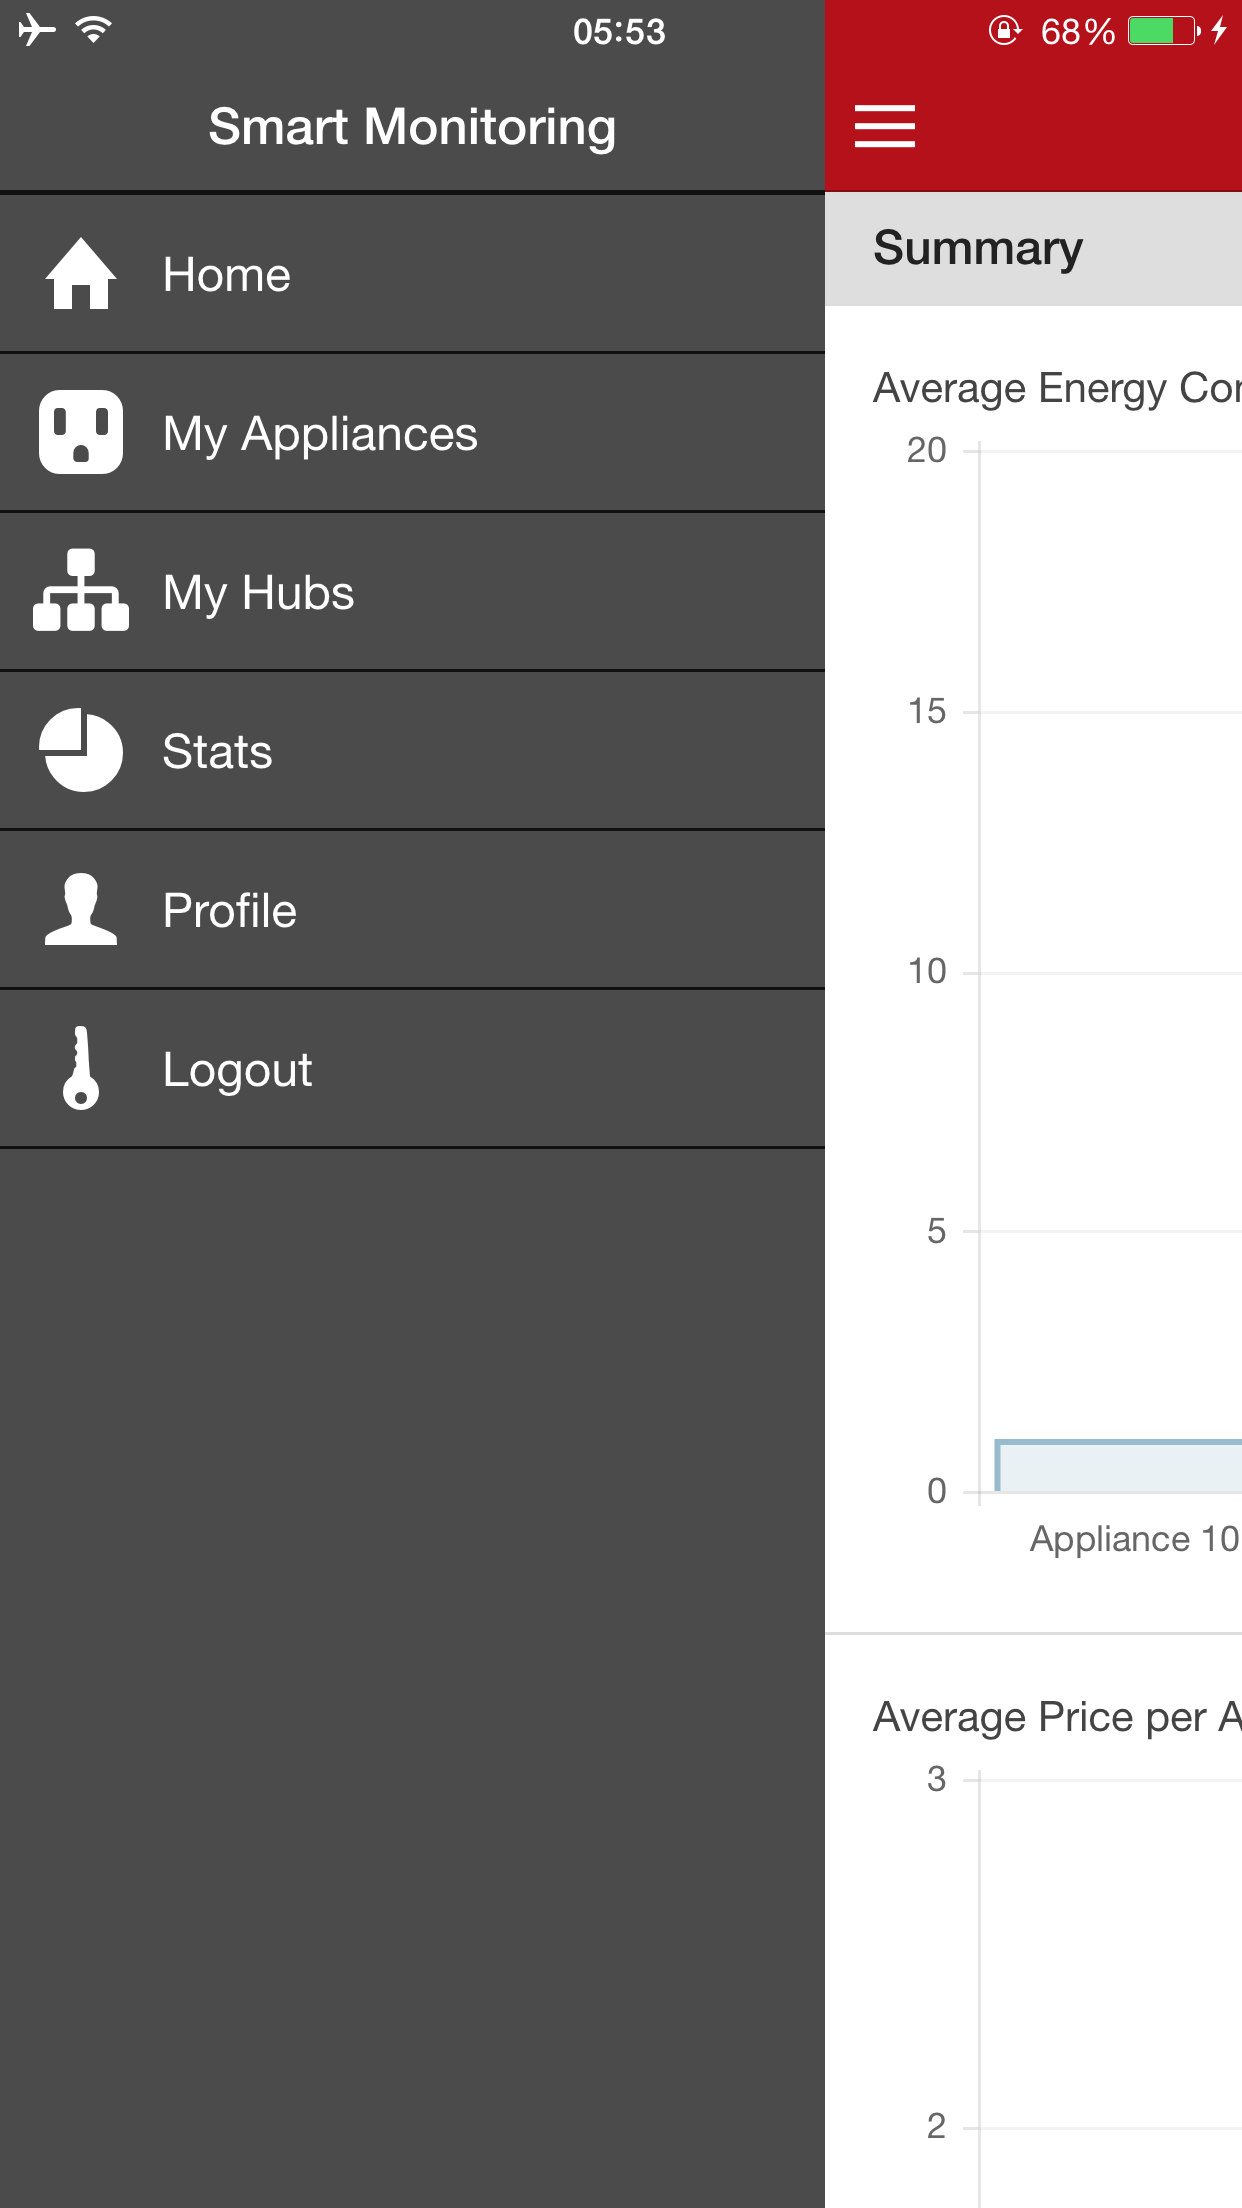
\includegraphics[width=\columnwidth]{/screenshots/hamburger}}
        \caption{The application "hamburger" menu view.}
    \end{subfigure}
    \caption{The home and menu views.}
    \label{fig:homemenu}
\end{figure}
In figure~\ref{fig:homemenu}.a, the home page is shown. The home page surmises core data from the server and displays statistics for the four most used fuses. At the time of this screenshot, data for only one fuse was available.\\
A key point to mention is the use of the drop down menu in the upper right hand corner of the screen to change the date, and ultimately the data. This is a common way of changing data sets used at many points in the application.\\
Figure~\ref{fig:homemenu}.b shows the hamburger menu, named because of the icon used to access it - three lines that are stacked. This menu is common place in many popular applications on both Android and iOS platforms, adhering to the heuristic of consistency and standards~\cite{nielsen}.\\
The menu is the main method of navigating the main features of the application. To make navigation easier, icons have been used based on the rule of recognition rather than recall proposed by Neilsen~\cite{nielsen}.\\
The "My Fuses" option has the same icon as that used in the application icon and splash screen in~\ref{fig:iconsplashlogin}.a and~\ref{fig:iconsplashlogin}.b.\\ 
The "My Hubs" icon is symbolic of that of a centralised system where all of the fuses report to a single point.\\ 
The remainder of the icons used are common place in the industry, and matches the users' understanding between the system and the real world~\cite{nielsen}.


\paragraph{Fuse views}
\begin{figure}[H]
    \centering
    \begin{subfigure}[t]{0.32\columnwidth}
        \centering
        \frame{
\includegraphics[width=\columnwidth]{/screenshots/fuses}}
        \caption{The list fuses view.}
    \end{subfigure}
    \begin{subfigure}[t]{0.32\columnwidth}
        \centering
        \frame{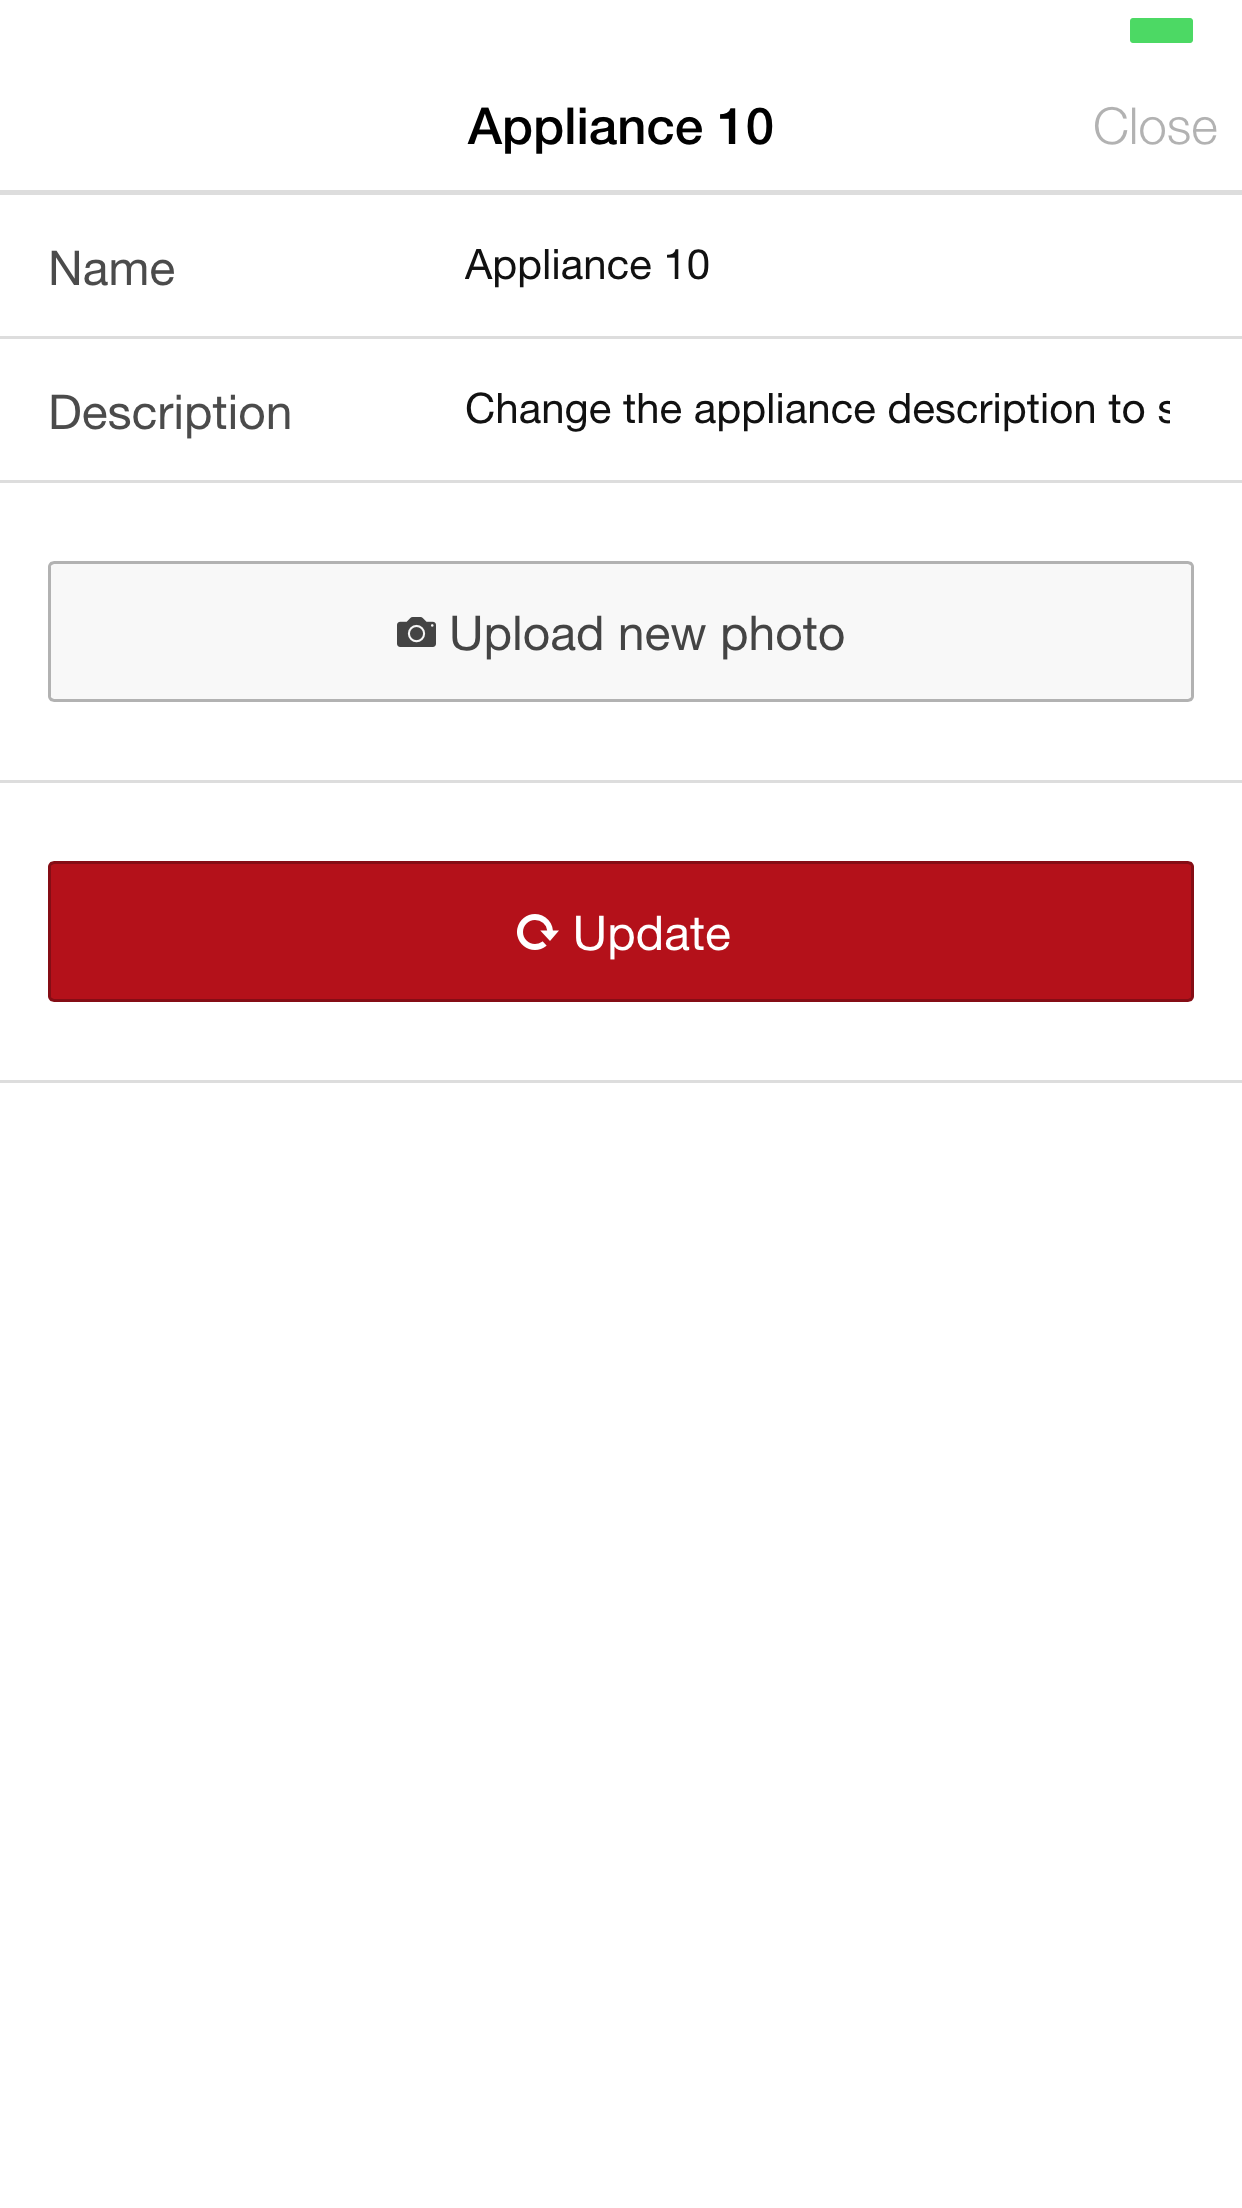
\includegraphics[width=\columnwidth]{/screenshots/editfuse}}
        \caption{The edit fuse view.}
    \end{subfigure}
    \begin{subfigure}[t]{0.32\columnwidth}
        \centering
        \frame{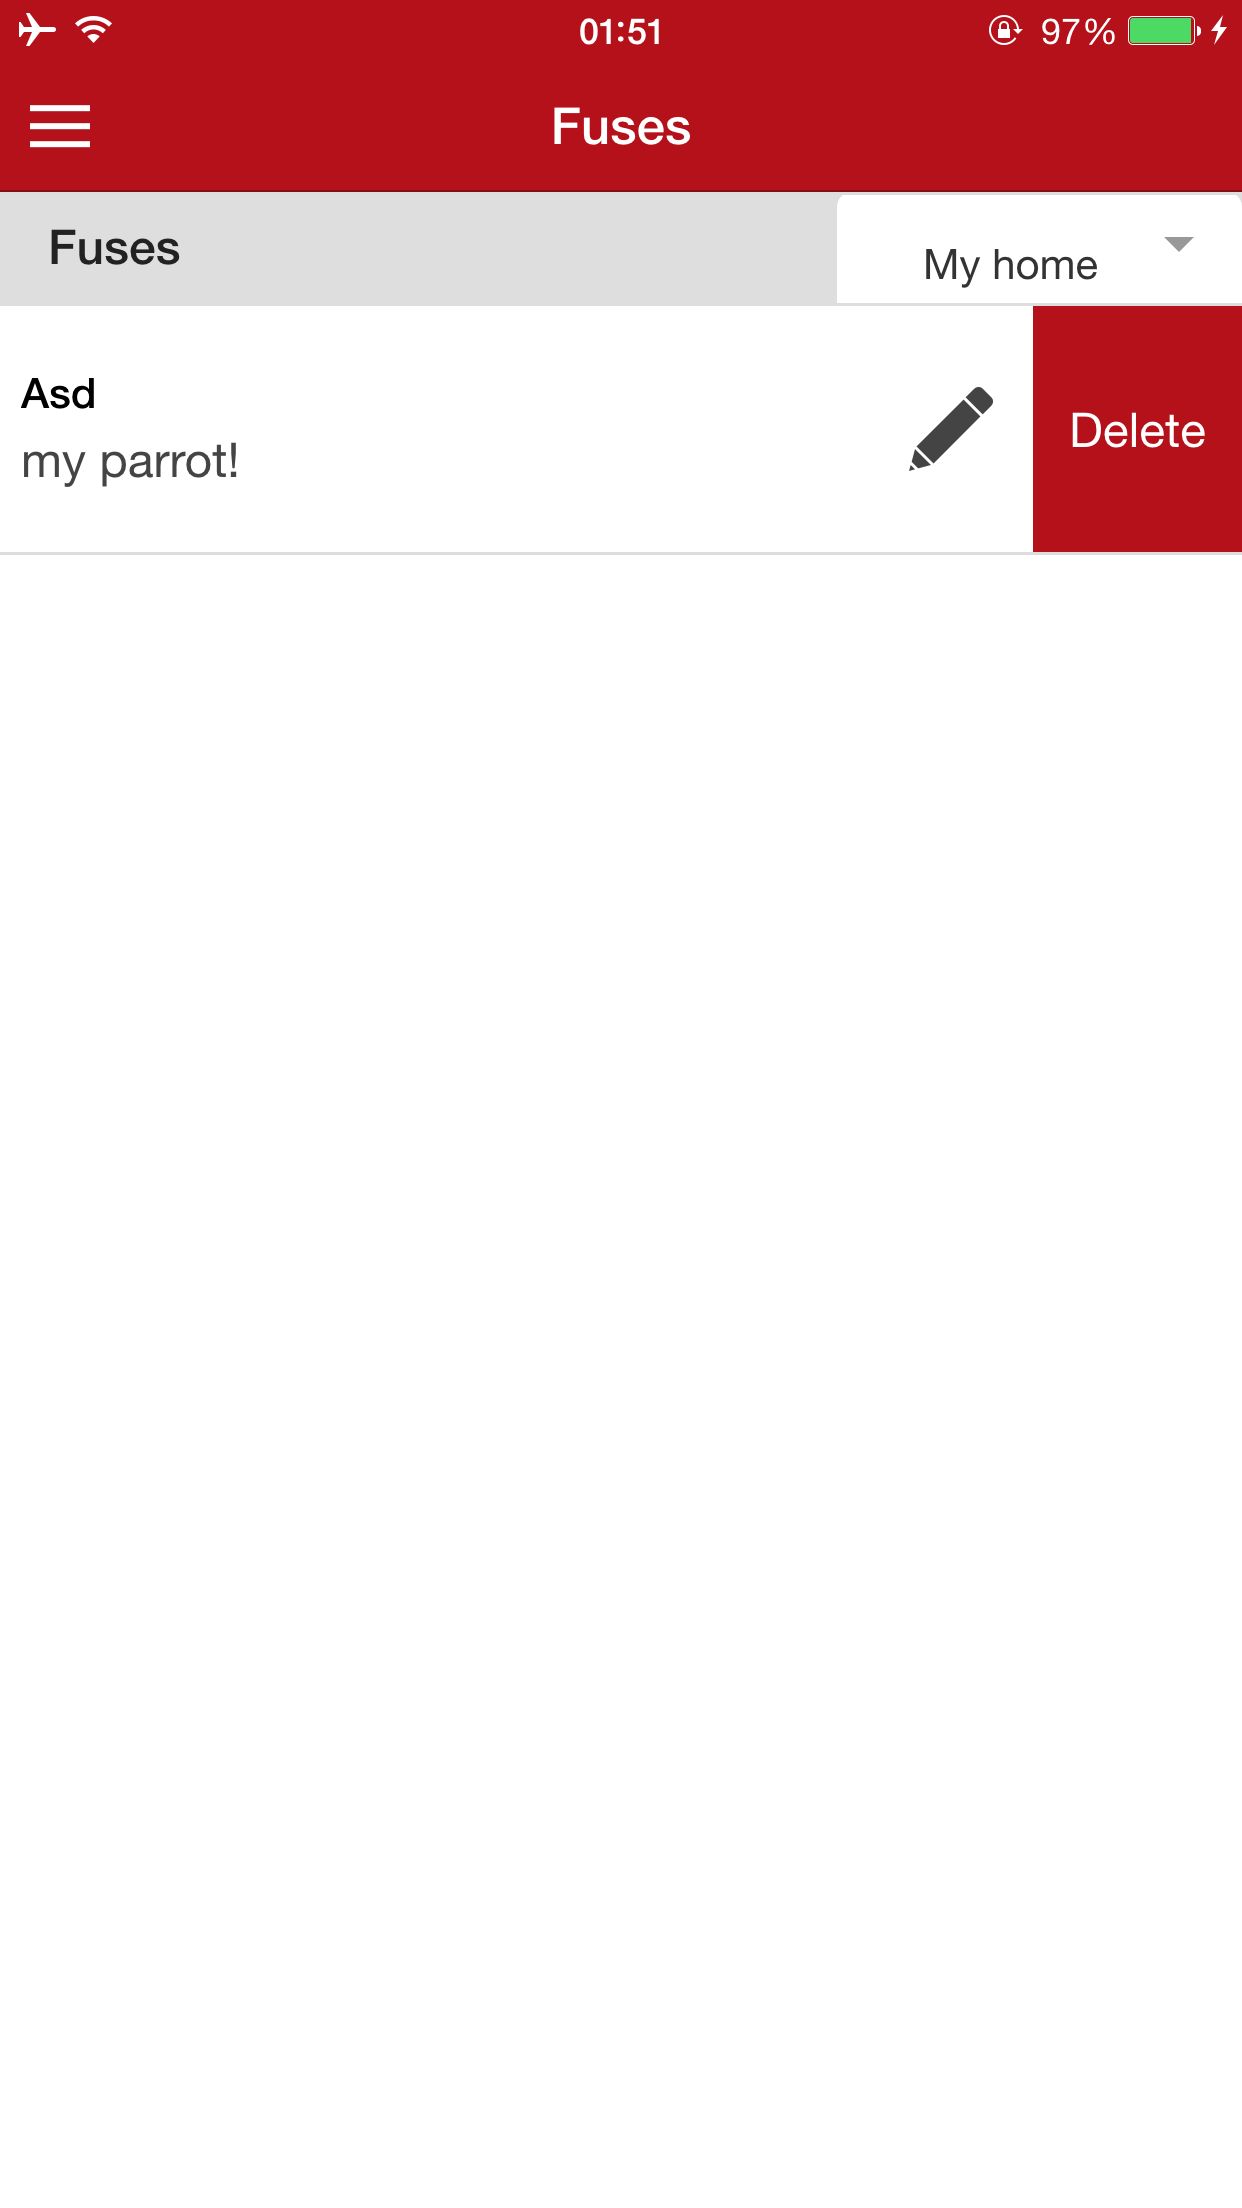
\includegraphics[width=\columnwidth]{/screenshots/deletefuse}}
        \caption{Removing a fuse.}
    \end{subfigure}
    \caption{The fuse views.}
    \label{fig:fuseviews}
\end{figure}
The listing of the fuses in figure~\ref{fig:fuseviews}.a allows the user to perform a number of actions:
\begin{itemize}
\item A tap on the individual fuse will display the live fuse view seen in figure~\ref{fig:deletelive}.b
\item A tap on the pen will launch the edit view seen in figure~\ref{fig:fuseviews}.b
\item A swipe on the list item will reveal the delete option seen in figure~\ref{fig:fuseviews}.c
\end{itemize}
All of the above actions are familiar throughout applications on both iOS and Android. The tap to view an item behaviour is seen on every single application that implements a list view, the tap the pen to edit motif is also present in many applications, and finally the swipe to delete behaviour is seen in the messages application on both platforms.\\
As mentioned in the section discussing the home view, there is the recurring drop down list in the upper right hand corner adhering to the heuristic of consistency and standards~\cite{nielsen}. In this view, it allows a user to switch between various hubs that may be linked to the user account.\\
Figure~\ref{fig:fuseviews}.b allows a user to change the name, the description and upload an image for the selected fuse. By default the fuse name is set to "Fuse \{Fuse ID\}", and the description is set to "Change the fuse description to something more meaningful", with the default image set to a question mark to indicate to the user they should change the data.\\
The idea behind having a picture for a Fuse was to allow a user to quickly identify specific appliances connected to the fuse. For instance, if a Fuse was connected to a monitor, the user would take a picture of the aforementioned monitor. The picture, combined with the name and description fields would speed up fuse identification ten fold.\\
Figure~\ref{fig:fuseviews}.c shows the method of deleting a fuse, swipe to the left to reveal the delete action. When the delete button is pressed, a confirmation box appears to ensure that the user wants to carry out the delete action, this can be seen in figure~\ref{fig:deletelive}.a. This feature is used to prevent user errors in accordance with Nielsens Heuristics~\cite{nielsen}.

\begin{figure}[H]
    \centering
    \begin{subfigure}[t]{0.32\columnwidth}
        \centering
        \frame{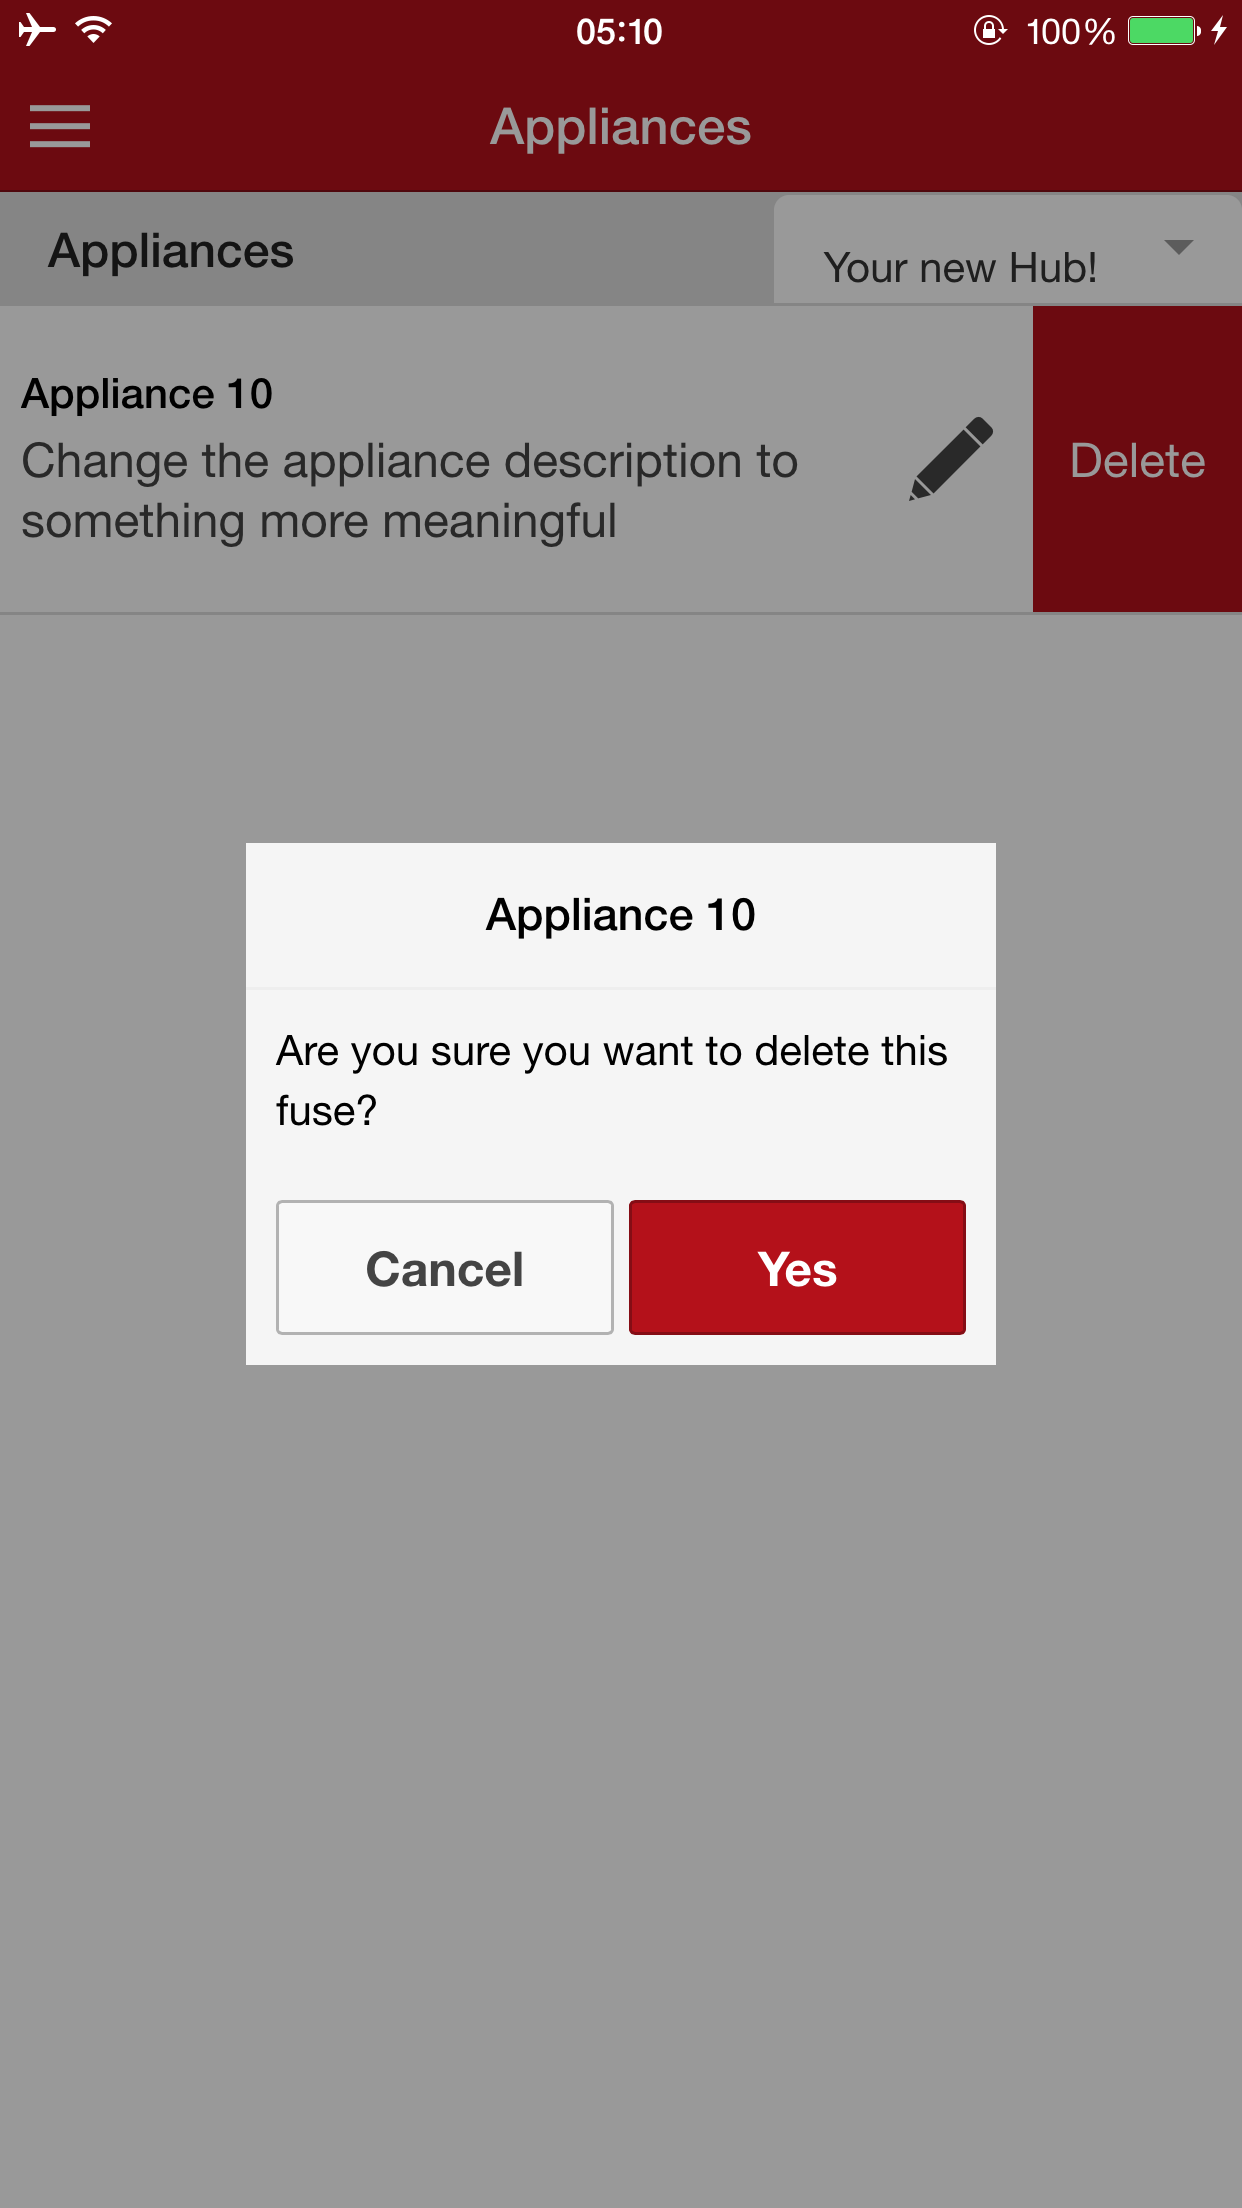
\includegraphics[width=\columnwidth]{/screenshots/areyousure}}
        \caption{UI prompt to ensure that the user wants to complete the delete action.}
    \end{subfigure}
    \begin{subfigure}[t]{0.32\columnwidth}
        \centering
        \frame{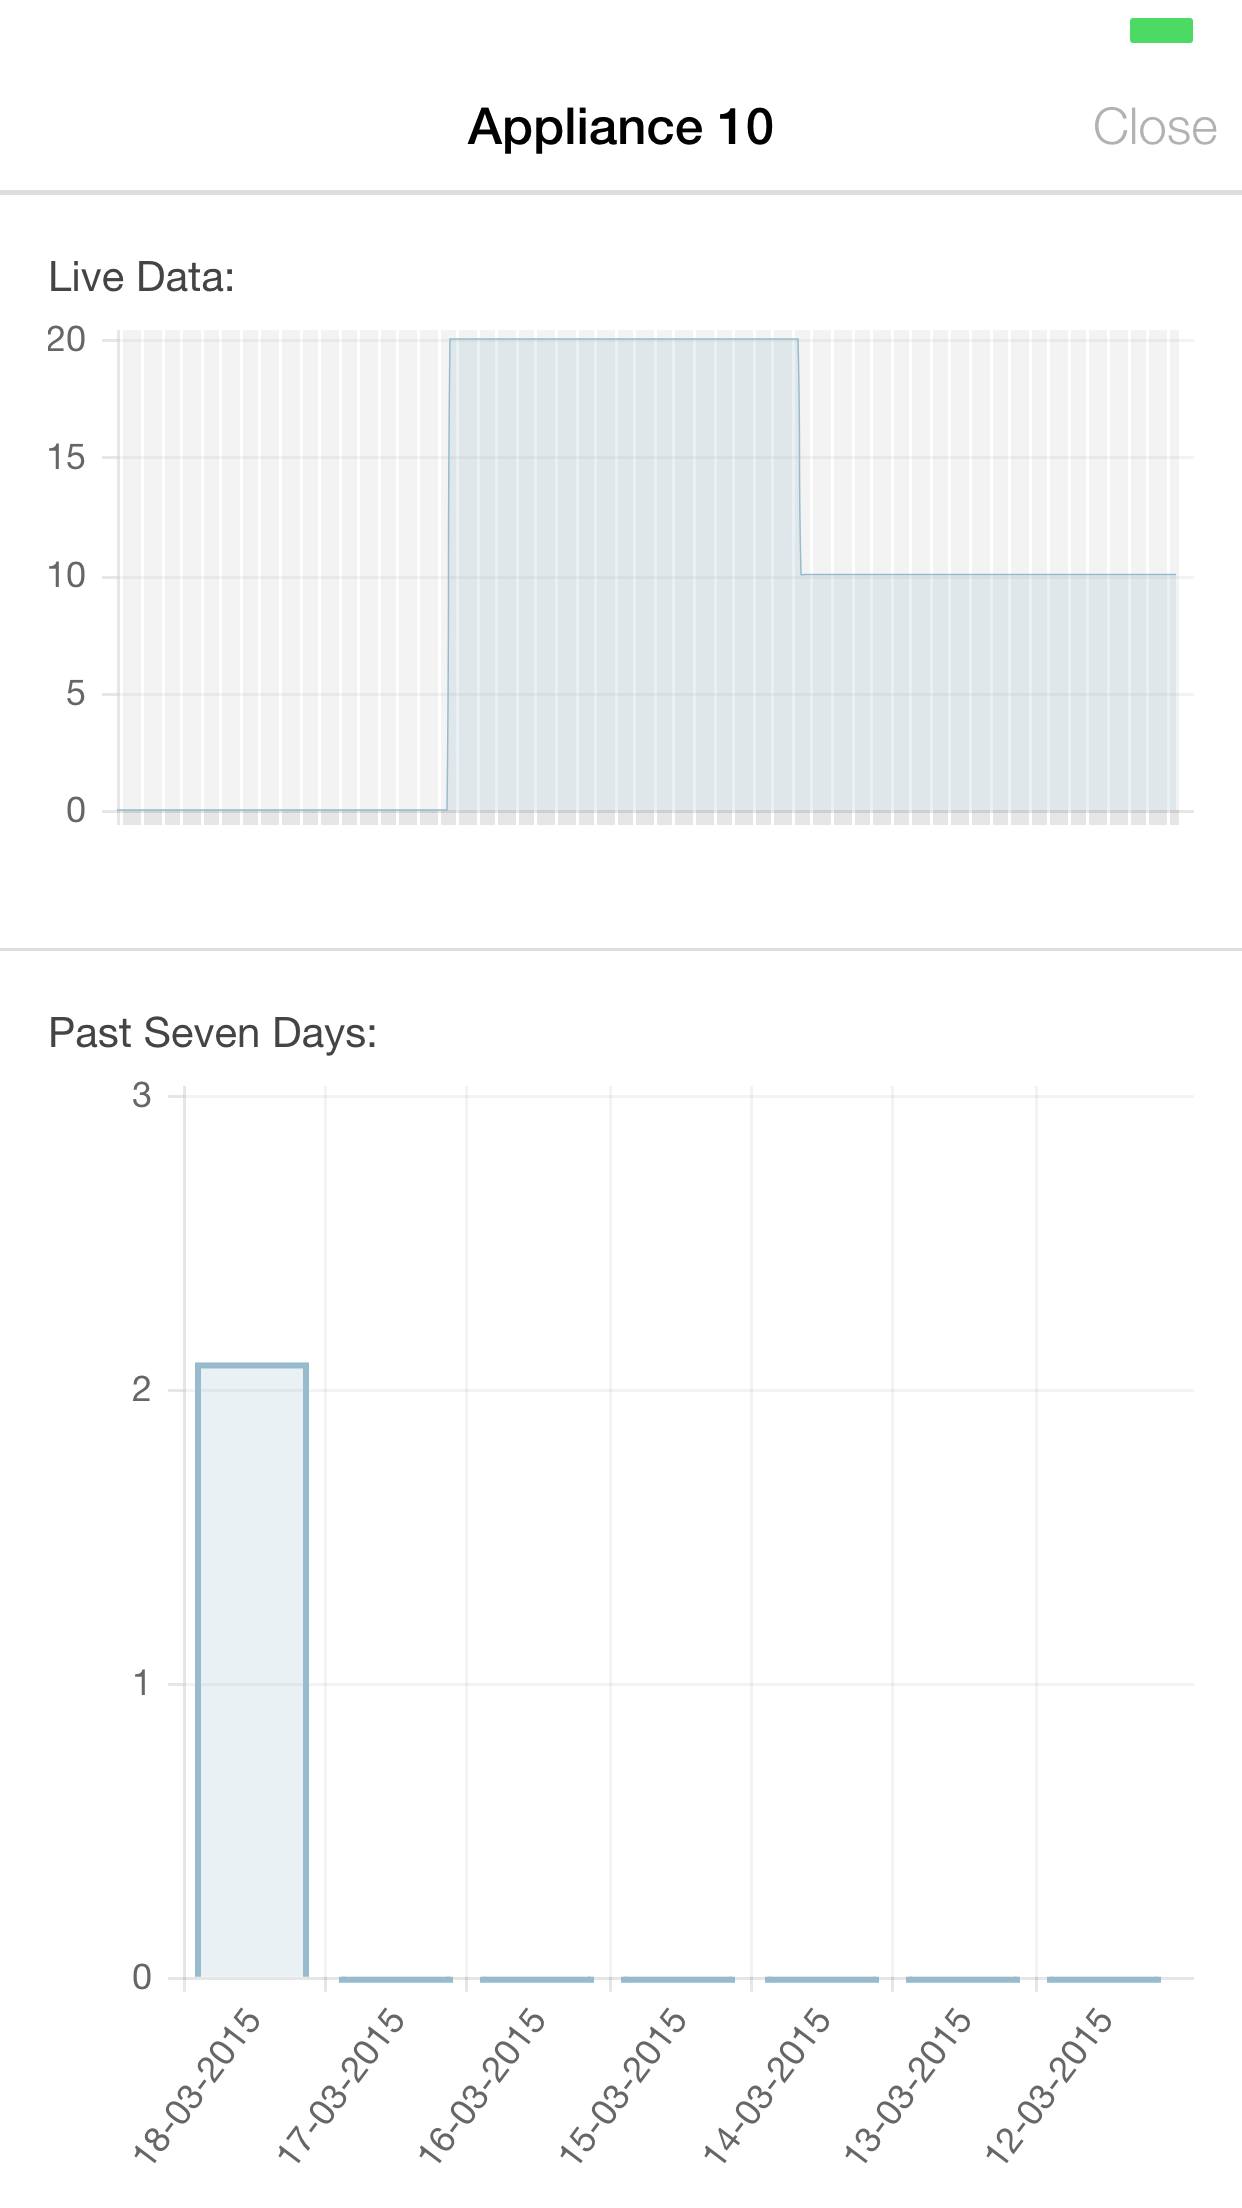
\includegraphics[width=\columnwidth]{/screenshots/live}}
        \caption{The live view and the summary of the past seven days for the selected fuse.}
    \end{subfigure}
    \caption{The 'Are you sure you want to delete view' and the live view of the data being reported by the selected fuse.}
    \label{fig:deletelive}
\end{figure}
Figure~\ref{fig:deletelive}.b shows the live data view and the seven day summary for the fuse titled 'Asd'. As a hub reports data for the selected fuse, the application will be notified, and the data will appear in the live view.\\
The seven day summary displays the average voltage over the past seven days for the selected fuse.

\paragraph{Statistics views}
\begin{figure}[H]
    \centering
    \begin{subfigure}[t]{0.32\columnwidth}
        \centering
        \frame{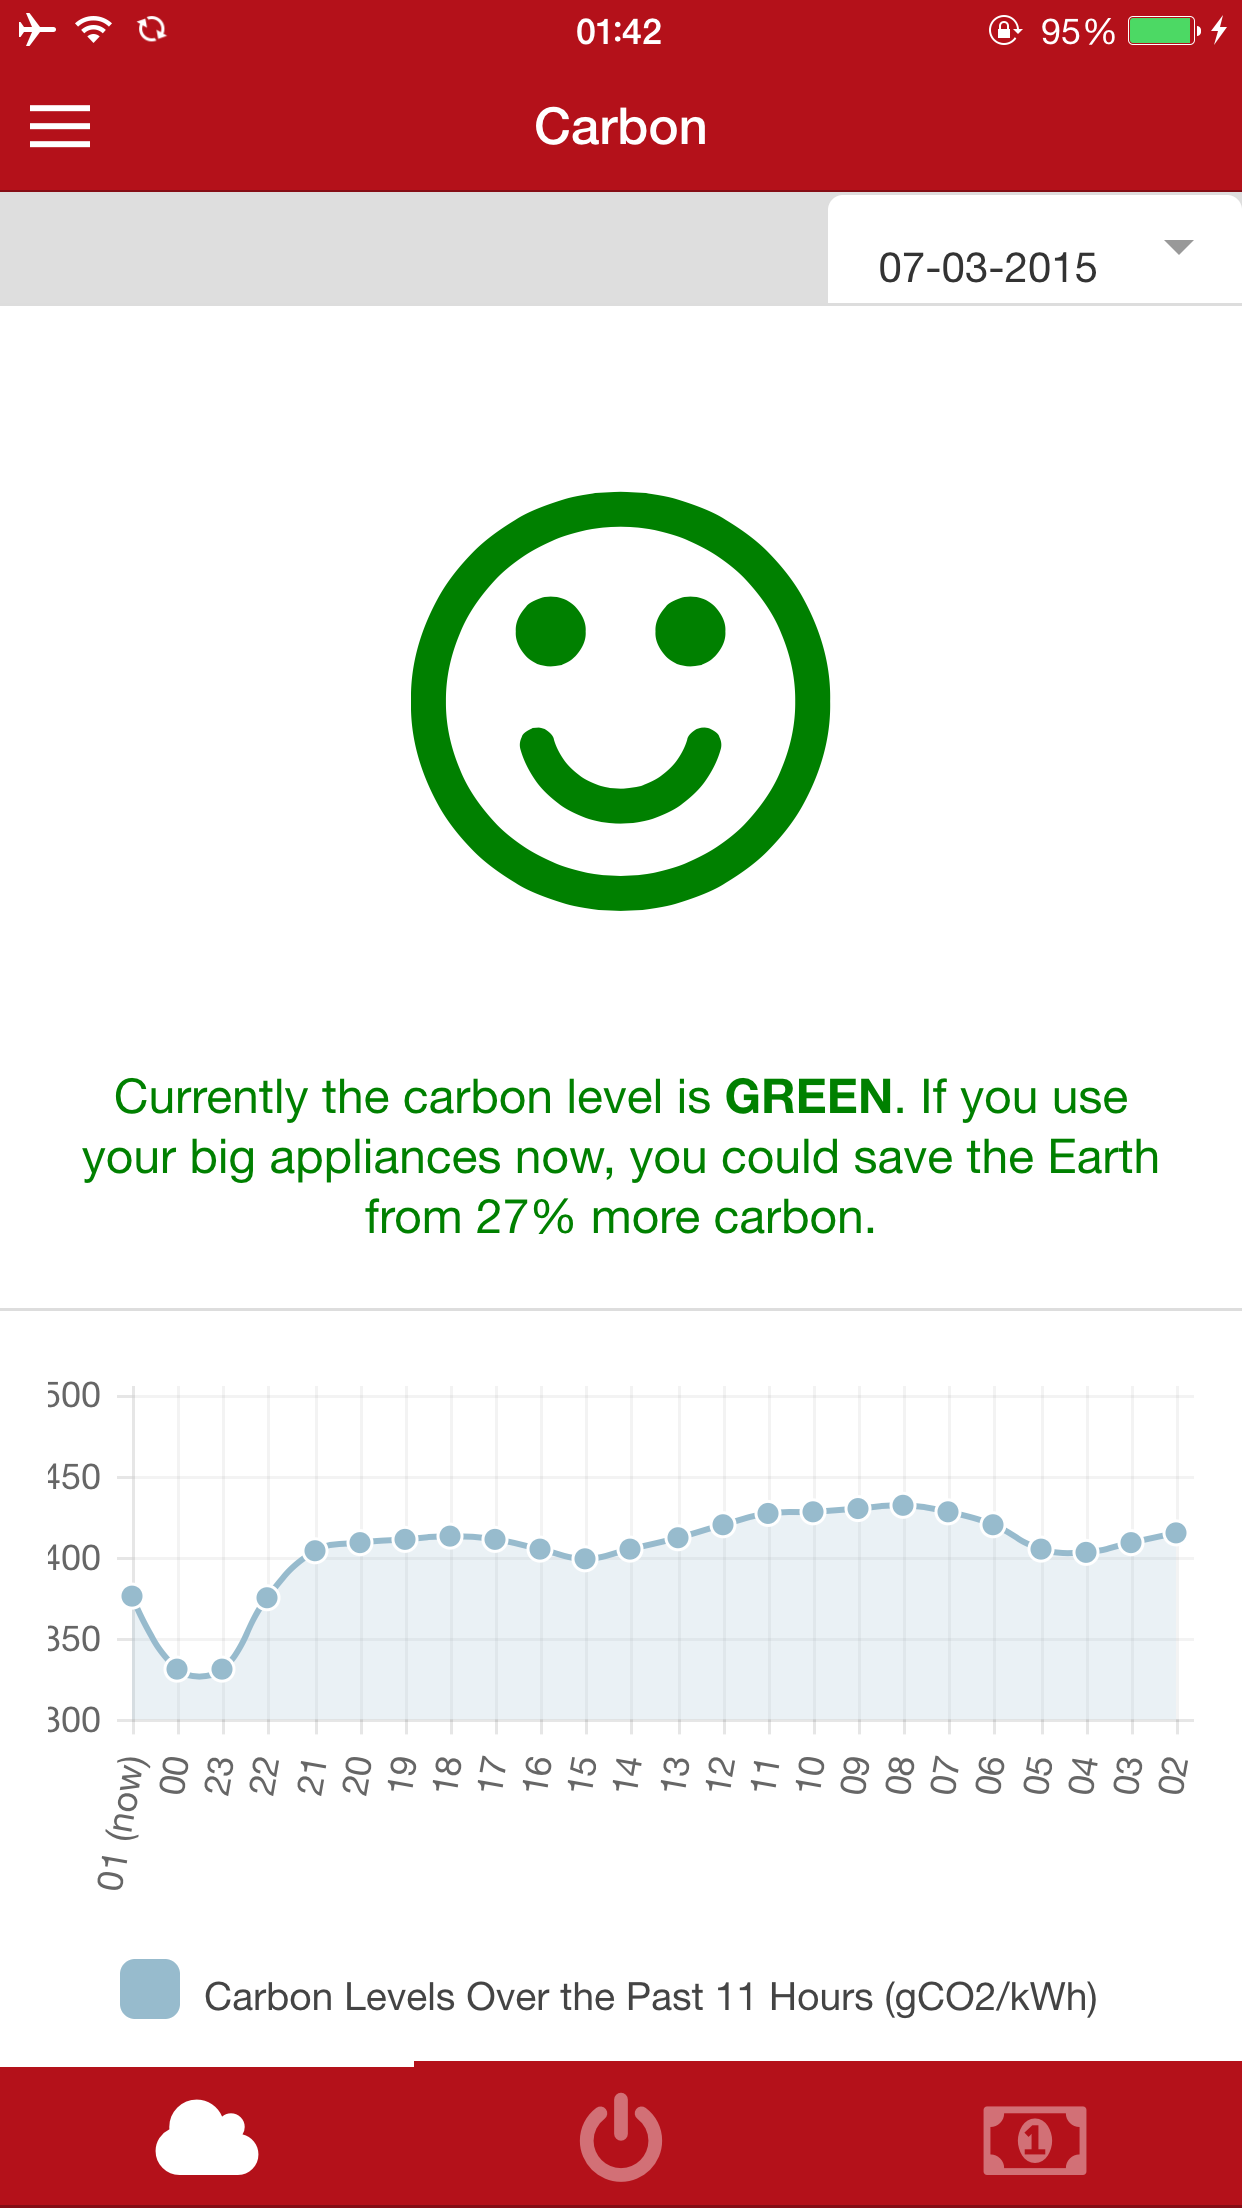
\includegraphics[width=\columnwidth]{/screenshots/carbon}}
        \caption{The carbon level statistics view.}
    \end{subfigure}
    \begin{subfigure}[t]{0.32\columnwidth}
        \centering
        \frame{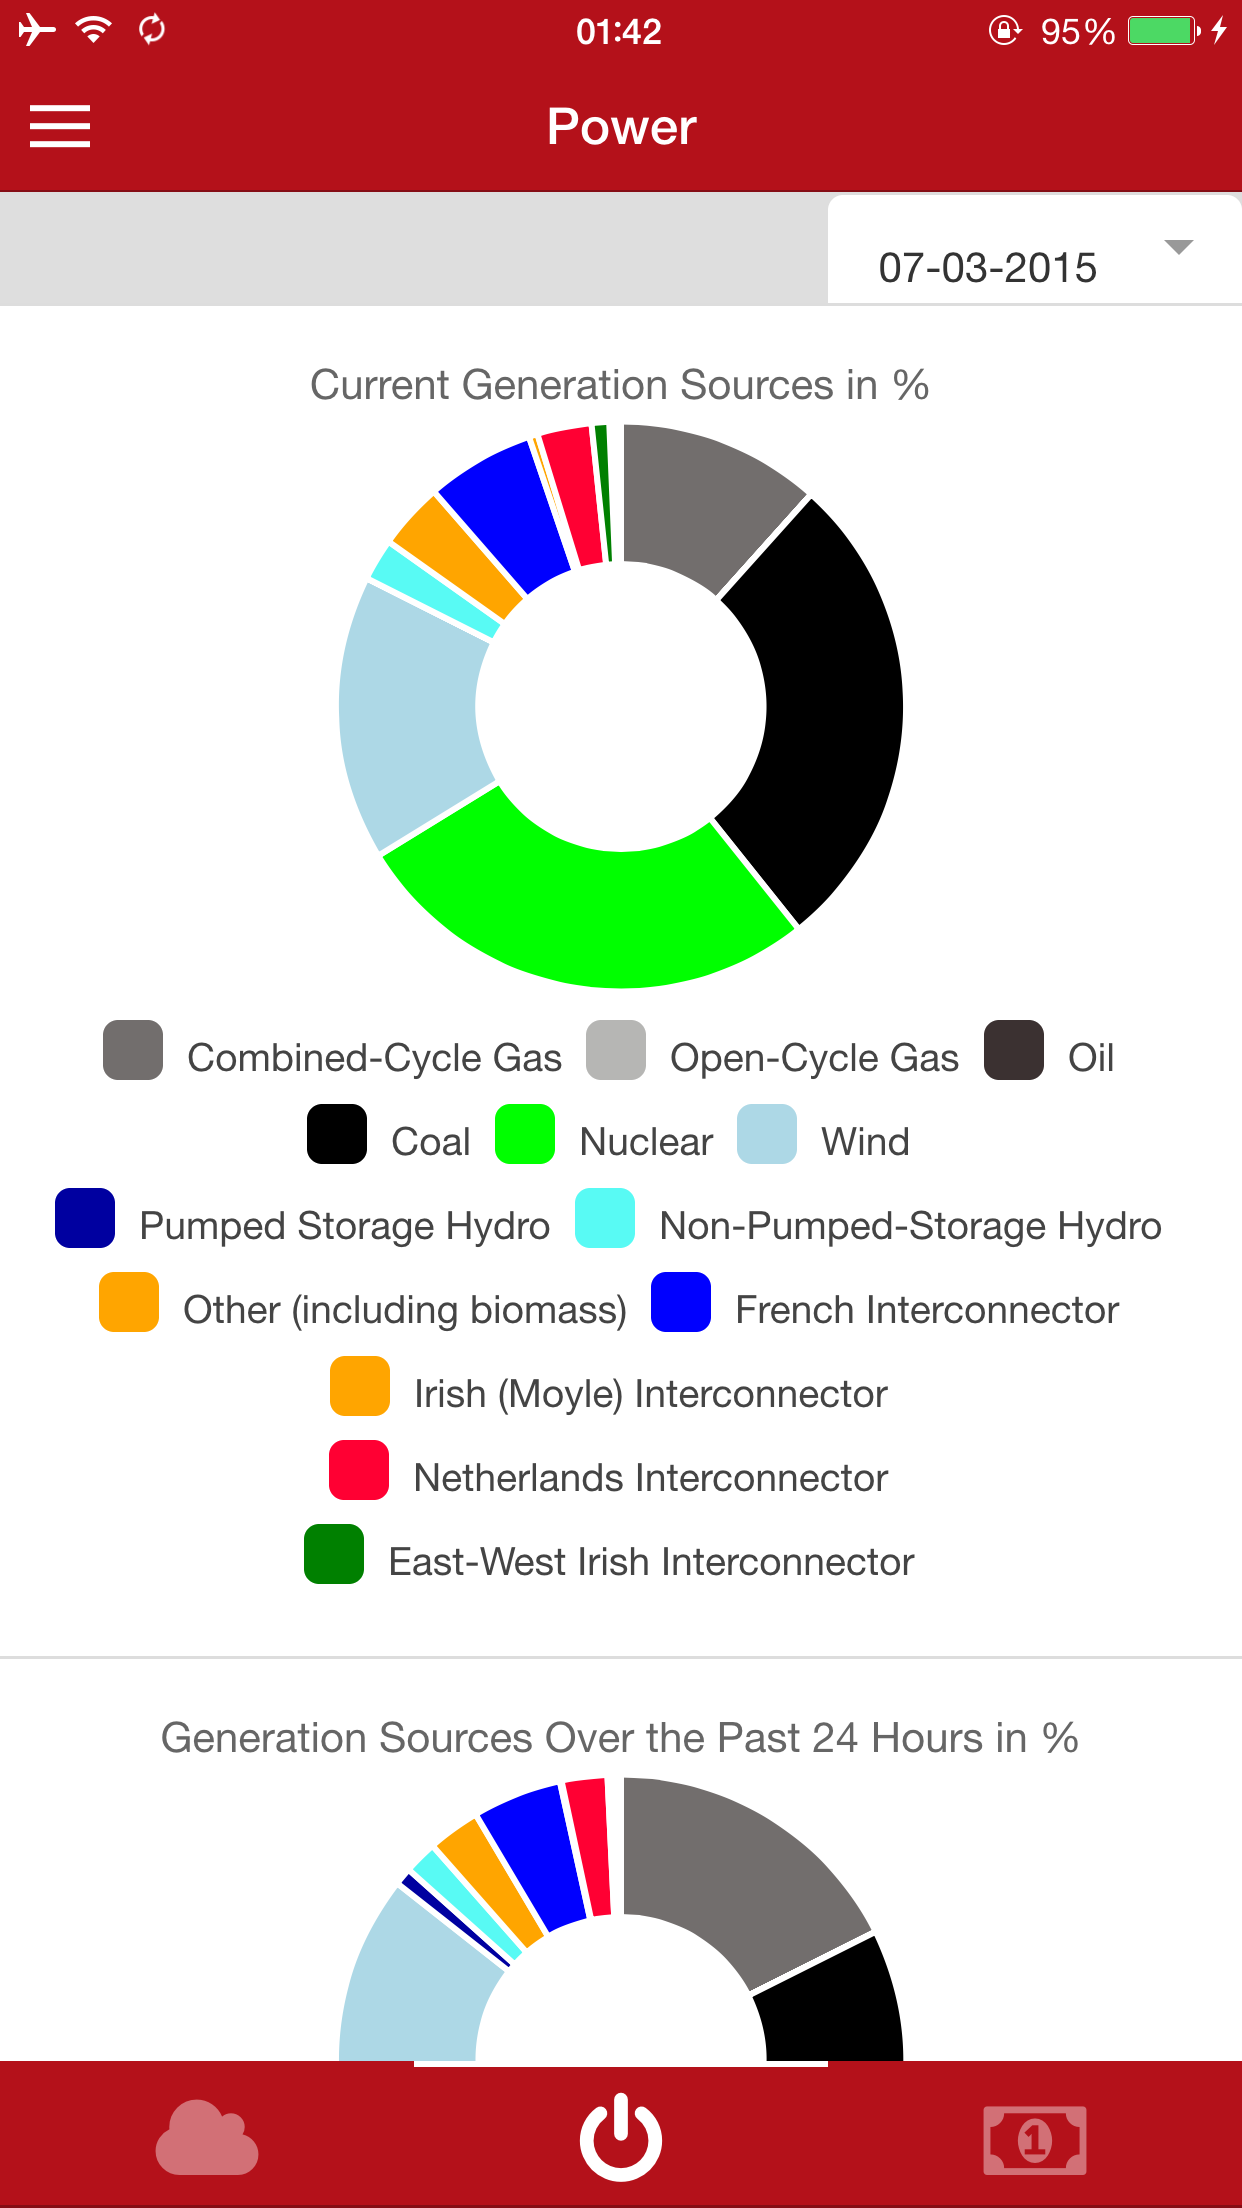
\includegraphics[width=\columnwidth]{/screenshots/power}}
        \caption{The power statistics view.}
    \end{subfigure}
    \begin{subfigure}[t]{0.32\columnwidth}
        \centering
        \frame{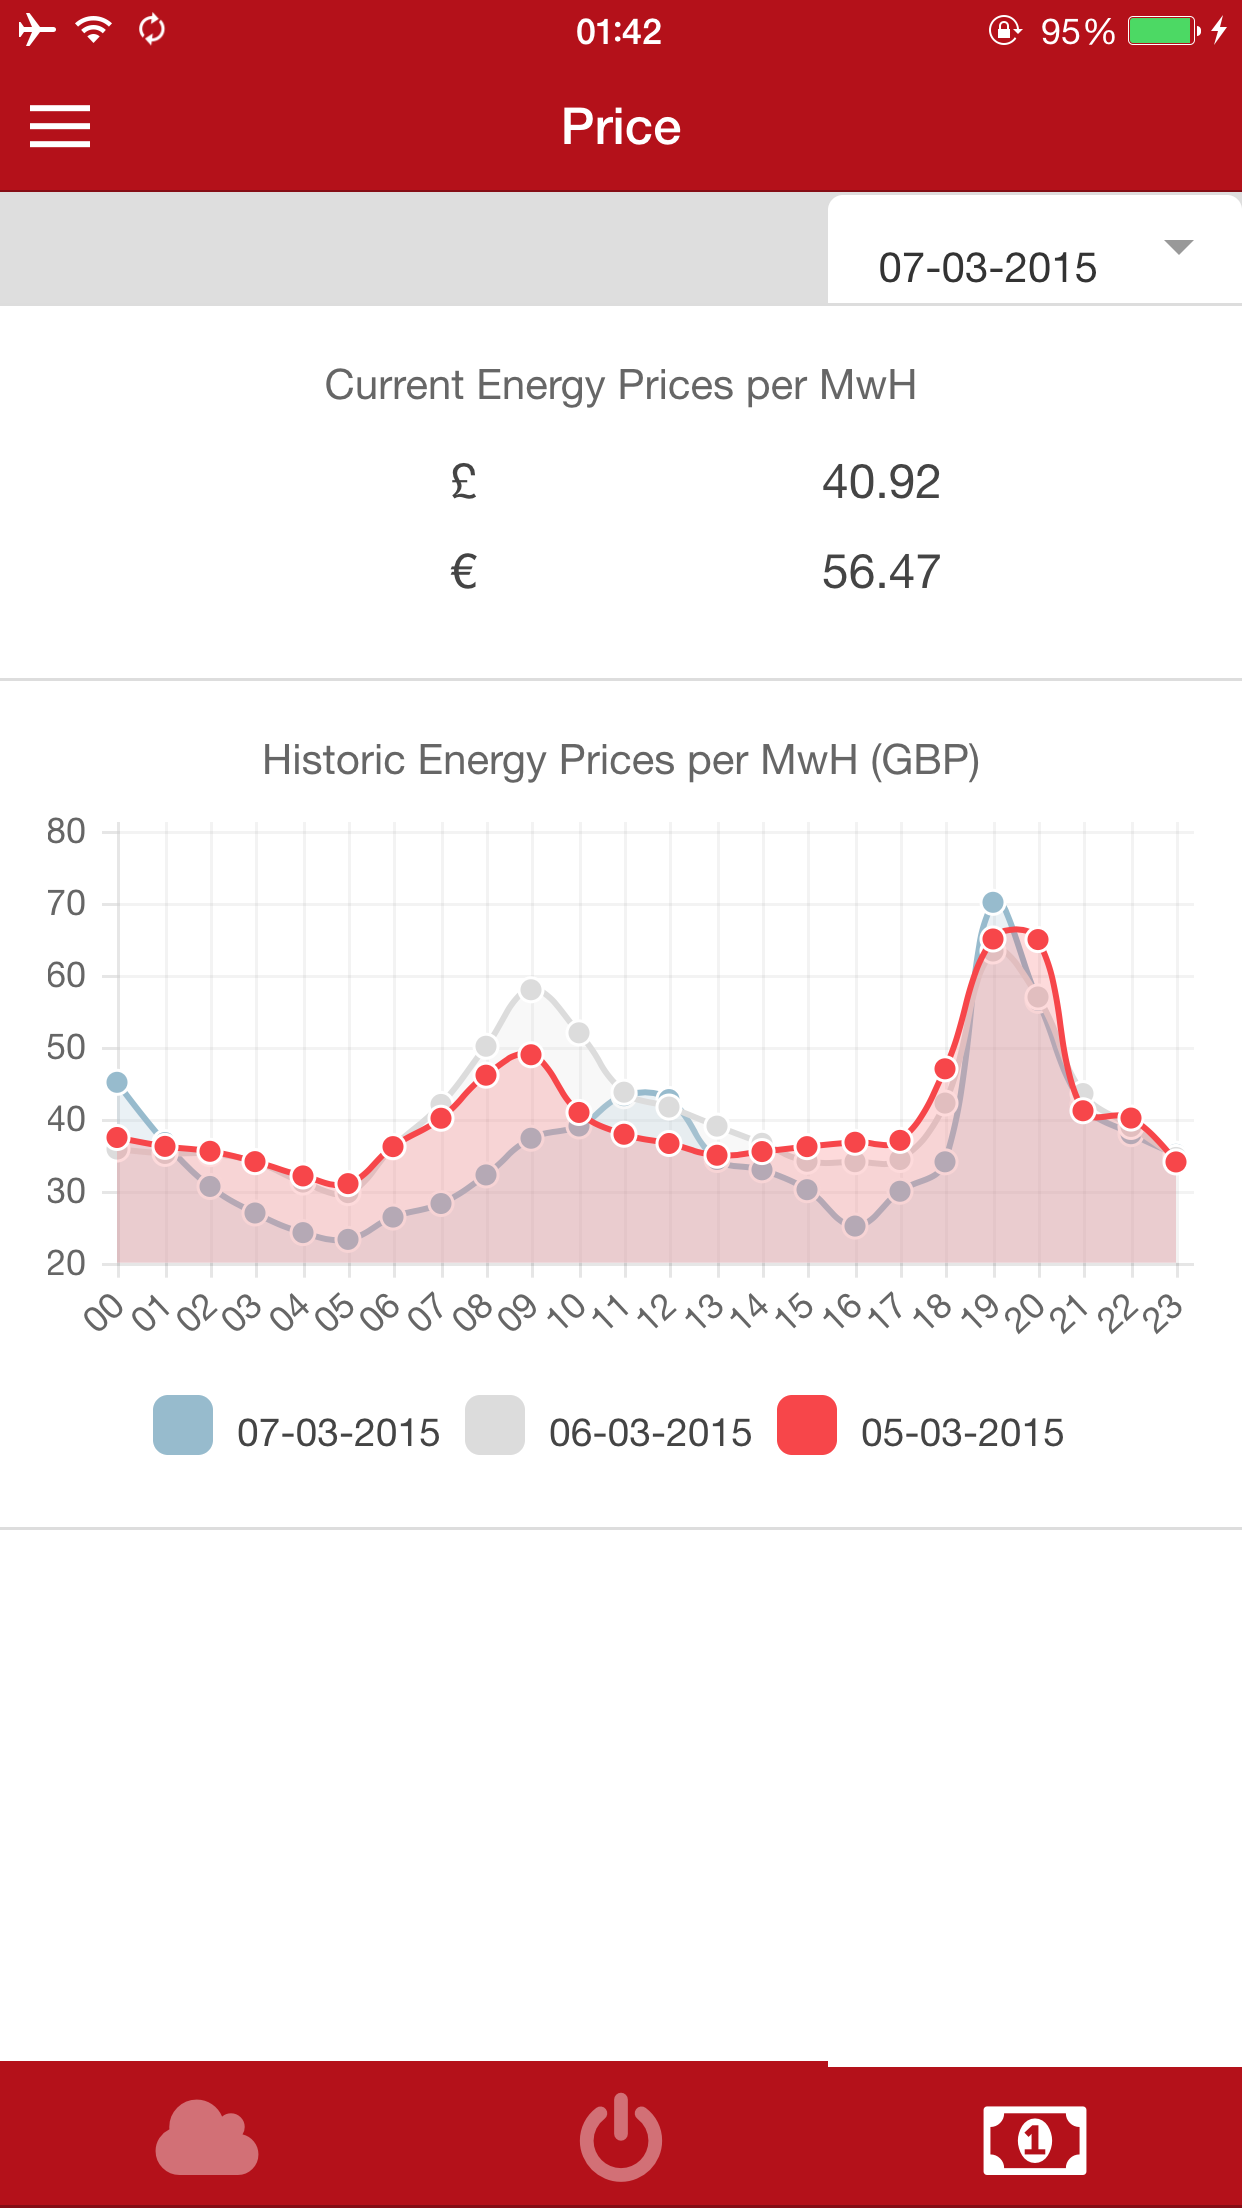
\includegraphics[width=\columnwidth]{/screenshots/price}}
        \caption{The price statistics view.}
    \end{subfigure}
    \caption {The statistics views.}
    \label{fig:statisticsviews}
\end{figure}
The statistics views are a really cool feature of the application. It allows a user to gain various insights into the current and historic carbon, power and price data. In the all three views date selection is available so that the user can look at information for previous days.\\
The aim behind this collection of views is to allow the user to evaluate the times at which they turn their big appliances on and off.\\
For the environmentally conscious, the carbon view (~\ref{fig:statisticsviews}.a) allows the user to see the live estimated level of carbon in the UK.\\ 
Throughout various points of the day, the level of carbon fluctuates.\\ 
If there is a high level of carbon, a red unhappy face is displayed, conveying to the user that the level of carbon is quite and the use of big appliances will make a large impact to the level of carbon. \\
If there is a medium level of carbon, an orange indifferent face is displayed, indicating that the level of carbon is moderate so the use of big appliances will make a small impact to the overall level of carbon.\\
If there is a low level of carbon, a green happy face is displayed as seen in figure~\ref{fig:statisticsviews}.a, this advises the user that the use of big appliances will make no significant difference to the overall carbon level.\\
The hope behind the availability of this statistic is to level out the carbon emissions throughout the day and change user behaviour so that the use of appliances is convenient to the planet, but not neccessarily to the user.\\
For users who are interested in where the sources of energy for the UK originate, the power view is available, seen in figure~\ref{fig:statisticsviews}.b. This view shows real time and historic power generation statistics for the UK in percent for each source of generation.\\
In the doughnut charts, there is a relation between the colour and each source of generation. Coal fueled generation is represented by a black ring, nuclear power generation is represented by a luminescent green and so forth.\\
The final statistic shown in figure~\ref{fig:statisticsviews}.c is the price data. This view shows the historic prices for the past 24 hours as well as the current price.\\
From the graph, really interesting insights can be gleaned. Over time there are various points where there is a spike in energy prices, this is due to the load increasing on the UK's electricity grid. Common spikes are around 10/11 am and 6/7pm where activities like boiling kettles and cooking take place.\\
There is a lot of research currently being placed into this field in an effort to reduce these spikes, thereby reducing price, and the load on the energy grid. A lot of energy is also wasted during these spikes, as the grid uses a demand and response system to predict energy usage, increasing or decreasing energy generation accordingly, if not all of the energy is utilised, it will be burnt off as heat.\\
In 2010, a study of demand and response approaches to European energy generation occurred~\cite{demandresponse}. The paper concludes that outdated metering technologies mean that the average home owner  is not aware of the real time energy prices, and are not billed accordingly. Through the use of the data gathered by the project, it could allow companies to more accurately bill the home owner, as well as providing valuable insights into energy consumption.\\
If a home owner was also aware of the impact that their appliances have on the grid, this may prompt a change in user behaviour, or encourage people to buy less energy intensive appliances. For example, a slow boiling kettle would do wonders for the grid, as the intensity of the energy consumed would be slower, the only cost being time.


\paragraph{Profile and logout}
\begin{figure}[H]
    \centering
    \begin{subfigure}[t]{0.32\columnwidth}
        \centering
        \frame{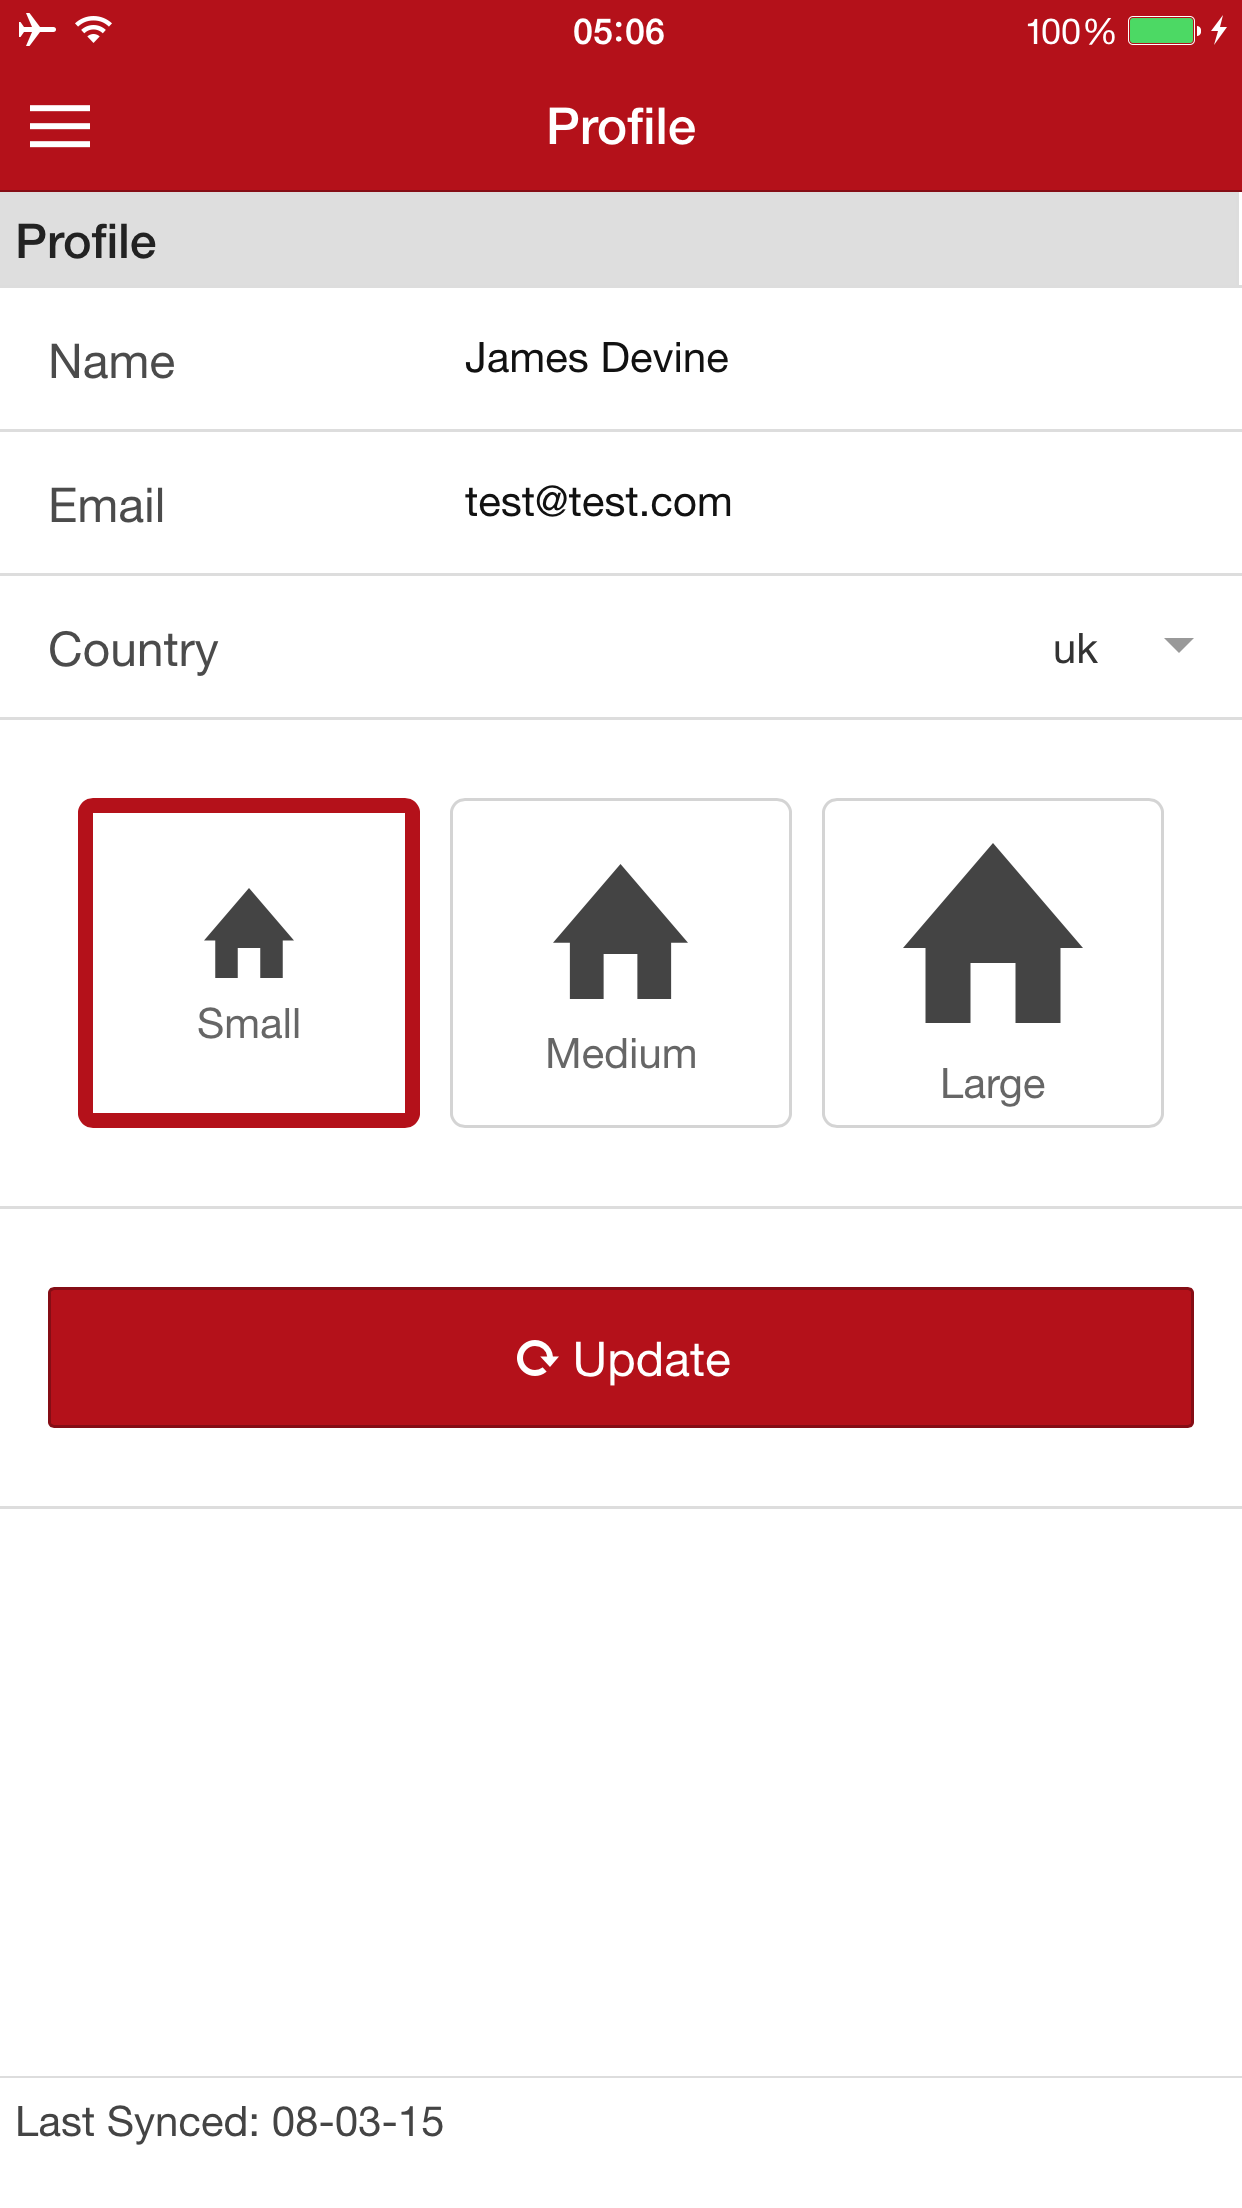
\includegraphics[width=\columnwidth]{/screenshots/profile}}
        \caption{The application profile view.}
    \end{subfigure}
    \begin{subfigure}[t]{0.32\columnwidth}
        \centering
        \frame{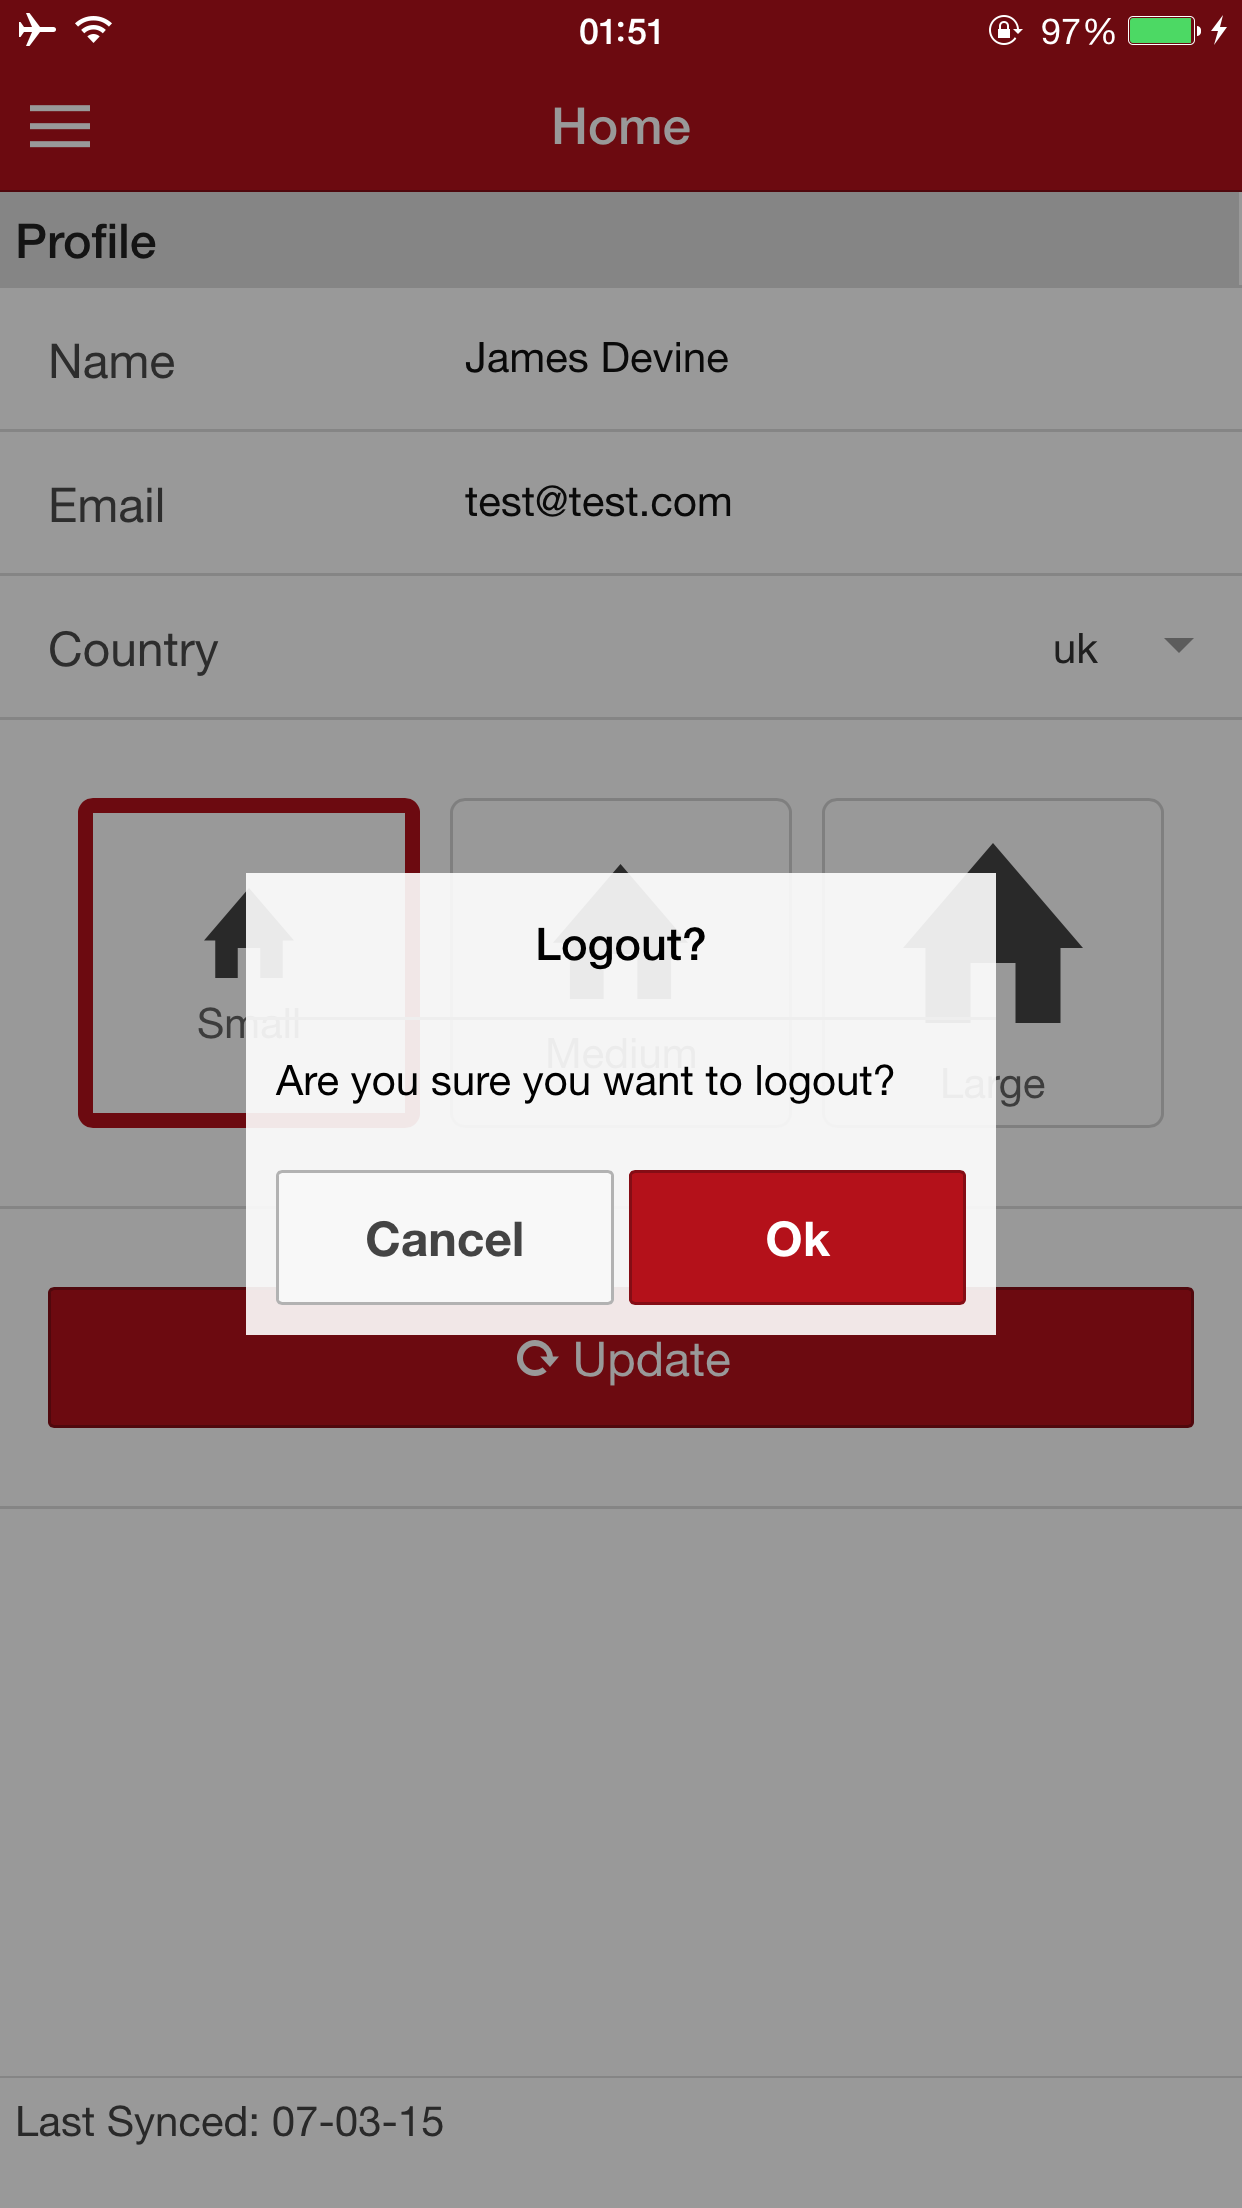
\includegraphics[width=\columnwidth]{/screenshots/logout}}
        \caption{The application logout view.}
    \end{subfigure}
    \caption{The profile and logout views.}
    \label{fig:profilelogout}
\end{figure}
The final two views of the application are the profile and logout views.
In figure~\ref{fig:profilelogout}.a the profile view can be seen. This allows a user to change their profile information stored on the server. They can change their name, their email address, their country and house size. The reason a users' country and house size are stored is because it acts as another metric for the energy suppliers to analyse.\\
The logout view in figure~\ref{fig:profilelogout}.b is accessible through the hamburger menu. The user will be asked if they would like to like out in order to prevent user error.\\
If a user clicks ok, all of the user information will be removed from local storage, the user will then be redirected to the login screen. If the user cancels the action, nothing happens. 


\subsection{Server}
The Server consists of a number of core elements: the Database, the Web Site and the API.\\
This section will breakdown these core elements and describe how the implementation of each came about, and the design of each.
\subsubsection{Requirements}
\begin{itemize}
\item \underline{Scalable} - The solution must scale to a number of servers, allowing for a distributed architecture.
\item \underline{Fast} - The solution needs to fast to minimise client hang time.
\item \underline{Development Time} - The speed of development for the chosen solution should be rapid to meet the tight time constraints of the project.
\item \underline{RESTful} - The application should be RESTful, using traditional HTTP methods and status codes to provide feedback to the application.
\end{itemize}
\subsubsection{Architecture Diagram}
\begin{figure}[H]
    \centering
    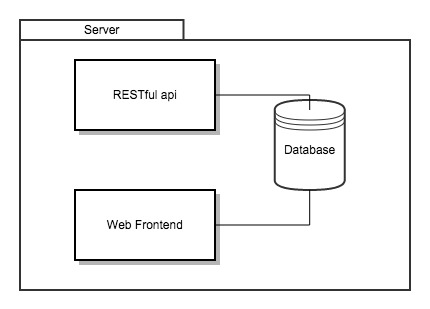
\includegraphics[width=8cm]{diagrams/server}
    \caption {Server Architecture Diagram}
\end{figure}

\subsubsection{Database}
\begin{figure}[H]
    \centering
    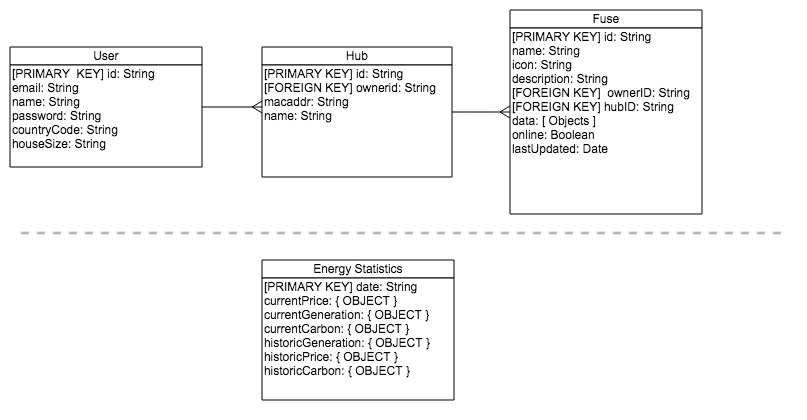
\includegraphics[width=\columnwidth]{diagrams/erd}
    \caption {Entity Relationship Diagram}
\end{figure}

The collection (database) contains four documents (tables) core to the operation of the platform.\\
The User document stores all details for the users registered with the platform, the Hub document stores all of the information that represents a Hub object and the Fuse document stores all of the details pertaining to a Fuse including the data transmitted from the Hubs.\\
The mappings between the documents are as follows:
\begin{itemize}
\item A User has a unique identifier.
\item A Hub has a unique identifier and also has an ownerid that maps onto the User document through the use of the UserID.
\item A Fuse has a unique identifier. A Fuse also contains an ownerID and a hubID which maps onto both the User document and the Hub document.
\end{itemize}
The documents were constructed in this manner because of a limitation with the implementation of the Fuse:\\
A Fuse can have an ID between 0 and 4095 ($2^{12}$). If a user had multiple installs in different locations, thereby requiring the use of more than one hub, without the Hub ID there could be duplicate Fuse IDs. A User also wouldn't want to see all of the Fuses for every single location.\\ 
Using the Hub document allows for the easy segmentation between locations and removes the possible collision of Fuse IDs.\\

The relationships between the documents are thusly:
\begin{center}
    \textit{"A User can have many Hubs and a Hub can have many Fuses"}
\end{center}
The Energy Statistics document is used to store data scraped from various APIs, which will be explained further on in this document.\\
Energy Statistics has a primary key of date, and bears no relation to any other documents. 

\subsubsection{Web Site}
Aside from the cross platform application, the server contains some additional front end user interfaces with the aims of detailing more information about the project, as well as allowing others to quickly register and join the project.\\

\begin{figure}[H]
    \centering
    \includegraphics[width=0.49\columnwidth]{/website/home}
    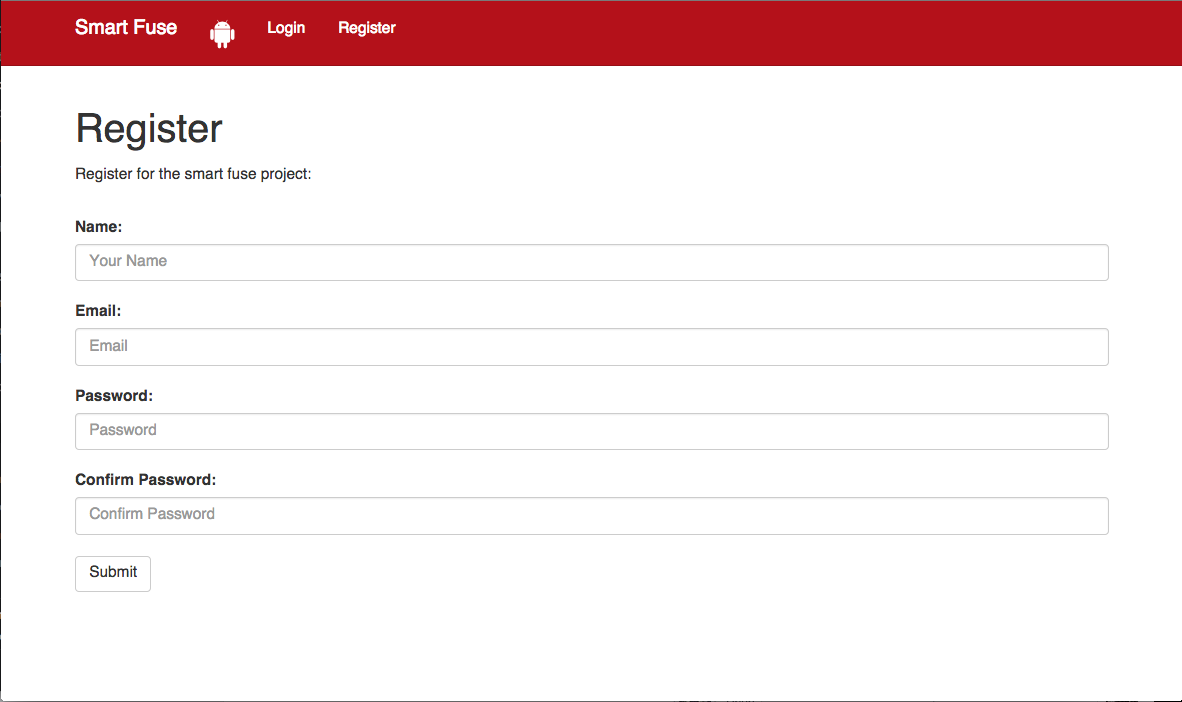
\includegraphics[width=0.49\columnwidth]{/website/register}
    \caption {The home and registration views of the site.}
\end{figure}
\begin{figure}[H]
    \centering
    \adjustbox{valign=t}{\includegraphics[width=0.49\columnwidth]{/website/login}}
    \adjustbox{valign=t}{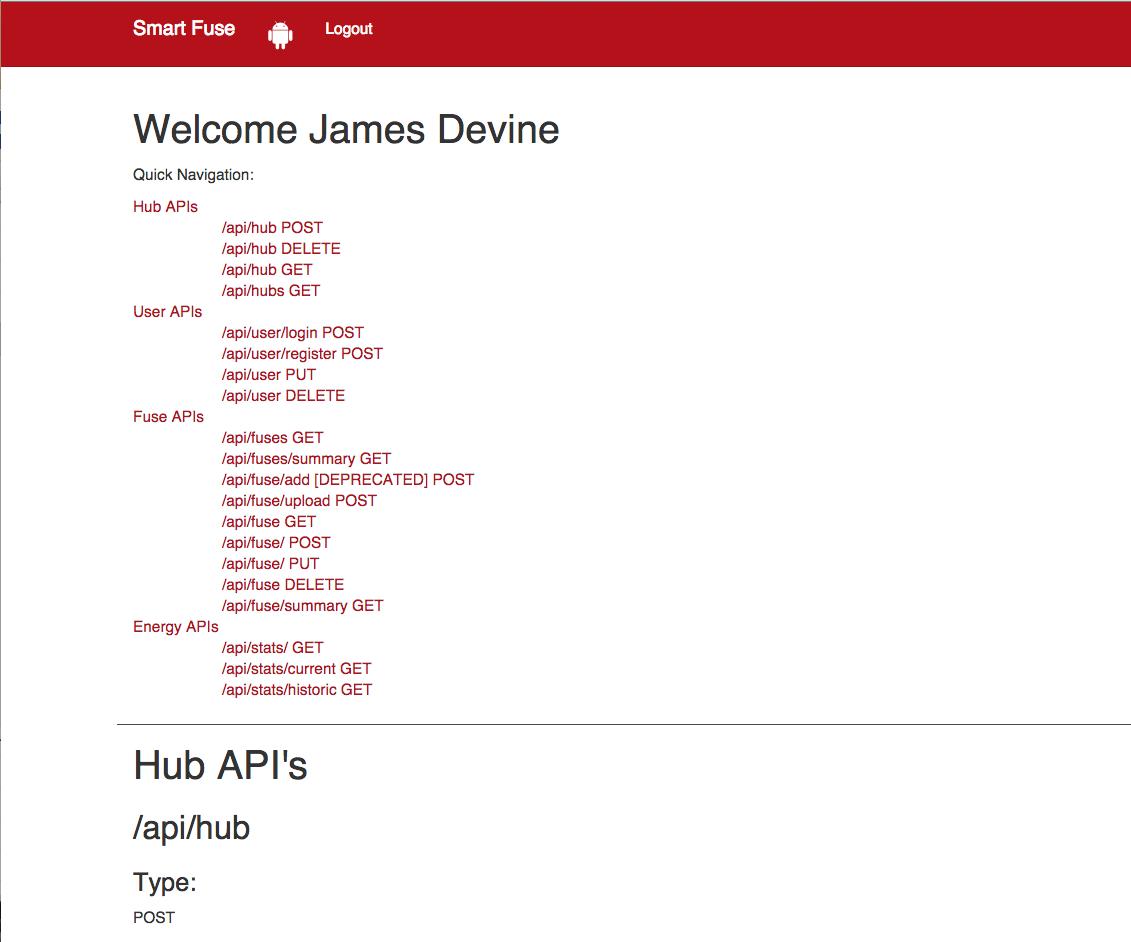
\includegraphics[width=0.49\columnwidth]{/website/api}}

    \caption {The login and home page after login.}
\end{figure}

The site is built using the Jade~\cite{jade} template engine and a customised bootstrap~\cite{bootstrap} theme, which means that the site is also responsive.\\
Users are able to download the most recent build of the android application from this site, unfortunately due to the restrictions imposed by Apple, the same cannot be said for the iOS version of the application.\\
Once a user logs in, the API documentation is then made available to them. A User can use this information to create their own applications, or recommend additional functionality. Users can also fork the project on Github, to collaborate and promote open source practices.

\subsubsection{Additional Features}

\paragraph{Socket.io}
Socket.io~\cite{socketio} is a javascript library compatible with both angular and node js. It allows bidirectional event-based communication between client and server.\\
Socket.io is used to update clients with real time data when a data point is added to a fuse by a hub, and the application is running.\\
Every time a user opens the app, they join a channel based on their user ID. When a data point is received, a look up is performed using the user ID provided in the /api/fuse POST request. The event is then broadcast down the channel if it exists, and is then digested by the client.

\begin{figure}[H]
    \centering
    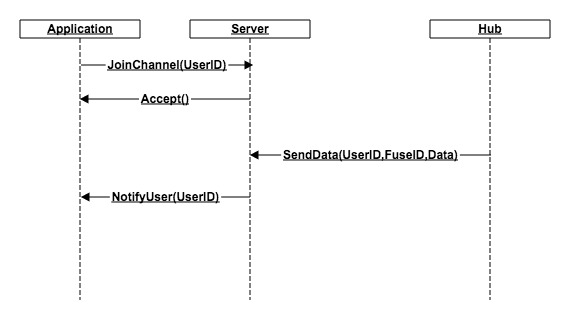
\includegraphics[width=\columnwidth]{/diagrams/socketio}

    \caption {The sequence diagram of live data reporting using Socket.io}
\end{figure}

Socket.io uses the well known method of long polling to keep connections open. It also enables the detection of disconnected clients through the use of a pulse every x seconds.

\paragraph{Data Scraping}

In order to produce the statistics seen in the application, the server is required to fetch data from a number of publicly available APIs.\\
If the current minute is: 0, 15, 30 or  45, the server harvests data from the following URLs:
\begin{itemize}
\item \url{http://www.earth.org.uk/_gridCarbonIntensityGB.xml}

\item \url{http://www.nordpoolspot.com/api/marketdata/page/1639}

\item \url{http://www.bmreports.com/bsp/additional/soapfunctions.php?element=generationbyfueltypetable}

\item \url{http://www.nordpoolspot.com/api/marketdata/page/4708}
\end{itemize}
All of the APIs return data in XML format. The server transposes them into easy to digest JSON objects, and stores them in the database to be retrieved by clients at a later date.\\

\paragraph{Adding Fuse Data Points}
When a Hub reports a data point for a fuse, the server optimises the packet to decrease the number of data points stored server side. The main reason for implementing the system in this manner entirely rests on time constraints for the project. There wasn't enough time to get the rigorous infrastructure in place to support such large amounts of data, whilst maintaining a fast API.\\
This optimisation is a summed average of the data points over a configurable period of time and is as follows:

\begin{equation*} 
\text{average voltage } = \cfrac{\text{sum of the reported voltages}}{\text{number of samples}}
\end{equation*}

The configurable period variable dictates the number of available samples for a given day. To calculate this value, the following will need to be evaluated:

\begin{equation*} 
\text{available samples } = \cfrac{\text{seconds in a day}}{\text{configurable period in seconds}}
\end{equation*}

In a full day there would be a total of 10800 samples for each Fuse if each Fuse transmitted data every 8 seconds.\\
Using the configurable period variable, the number of samples can be reduced significantly.\\
Currently, the configurable period is set to 10 minutes. Evaluating the previous calculation will result in the number of available samples to be determined.:

\begin{equation*} 
 \cfrac{86400}{\text{600}} = 144 \text{ samples}
\end{equation*}

Each sample would then contain the average of 75 data points reported by the Hub if the Fuses were reporting once in an 8 second interval.\\
The downside to this approach is that the platform will not immediately react to sharp changes in voltages reported by the Fuses. \\
An interesting point to mention, is that when a new data point is reported by a hub, the real time energy price is fetched and used to calculate the costing of that data point. This feature enables the Users to see accurately the price of the energy they are consuming. 
% BENEFITS ENERGY COMPANIES?

\subsubsection{RESTful API}

REST stands for Representation State Transfer and outlines a software architecture style for creating scalable web services.\\
REST is stateless, meaning that the clients' state isn't maintained by the server and is instead maintained client side.\\
True REST uses HTTP status codes and request types. The following request types and status codes are prominent throughout the API:\\

\underline{Request Types:}
\begin{itemize}
\item GET - Read an item.
\item POST - Create an item.
\item PUT - Edit an existing item.
\item DELETE - Remove an item.
\end{itemize}

Each request type above is used as specified by w3.org~\cite{w3}. The four request types map onto the essential CRUD operations that are performed in most data-oriented systems.\\

\underline{Status Codes:}
\begin{itemize}
\item 200 - Ok.
\item 201 - Created.
\item 400 - Bad request.
\item 403 - Forbidden.
\item 404 - Not found.
\item 500 - Internal server error.
\end{itemize}

The usage of the above status codes is in compliance with those specified by w3.org~\cite{w3}. They are used to provide primitive error detection capabilities to the client.\\
To ensure that all requests are valid, parameters are checked before carrying out every request, if one or more parameters are missing, the HTTP status code 400 Bad Request is returned.\\
Some requests like /api/fuses GET will return an empty array if there are no fuses available for a user instead of displaying an error code. This is intentional because the request has been successfully carried out, the result being that the user doesn't have any fuses.\\
Mostly when a transaction has been carried out successfully, the status code returned will be 200 Ok. There is an exception to this rule, like when performing a POST request. If the POST request is valid, a 201 Created status code will be returned indicating that the object has been created and is ready to use.\\
500 Internal Server Error is only returned when something unexpected has happened, and the server cannot fulfill the request.\\
Every time an API is called, the server provides additional feedback on the operation that just occurred on top of the HTTP status codes.\\
If an operation has been completed successfully the following JSON will be returned along with any additional data:\\[5pt]
\begin{minted}[frame=single,framesep=3mm,linenos=true,xleftmargin=21pt,tabsize=4]{js}
{success: "SUCCESS MESSAGE",....}
\end{minted}

If an operation fails to complete, the following JSON will be returned along with any additional data:\\[5pt]
\begin{minted}[frame=single,framesep=3mm,linenos=true,xleftmargin=21pt,tabsize=4]{js}
{error: "ERROR MESSAGE",....}
\end{minted}


\paragraph{Hub API's}
\subparagraph*{/api/hub}
\underline{Type:} \textbf{POST}\\

\underline{Description:} Links a users' account with a hub using the userID and the hubID. The hub can then be viewed in the application.\\

\underline{Parameters:}
\begin{itemize}
\item userID: A string containing the id of the user

\item hubID: A string containing the hub the user is trying to link
\end{itemize}
\underline{Expected Response:}\\[5pt]
\forceindent Status Code: \textbf{201} \\
\begin{minted}[frame=single,framesep=3mm,linenos=true,xleftmargin=21pt,tabsize=4]{js}
{success: "Hub added"}
\end{minted}

\underline{Error Response:}\\[5pt]
\forceindent Status Code: \textbf{400} \\
\begin{minted}[frame=single,framesep=3mm,linenos=true,xleftmargin=21pt,tabsize=4]{js}
{error: "Hub couldn't be added"}
\end{minted}



\subparagraph*{/api/hub}
\underline{Type:} \textbf{DELETE}\\

\underline{Description:} Removes a hub from the database, effectively unlinking a user account from the hub itself. The hub can still report data and will be aware that it is no longer linked to a user.\\
Any data prior to this request will be purged from the database.\\

\underline{Parameters:}
\begin{itemize}
\item userID: A string containing the id of the user. This is used to ensure that owners can't remove each others' hubs.

\item hubID: A string containing the if of the hub the user is trying to remove.
\end{itemize}

\underline{Expected Response:}\\[5pt]
\forceindent Status Code: \textbf{200} \\
\begin{minted}[frame=single,framesep=3mm,linenos=true,xleftmargin=21pt,tabsize=4]{js}
{success: "Hub removed"}
\end{minted}

\underline{Error Response:}\\[5pt]
\forceindent Status Code: \textbf{400} \\
\begin{minted}[frame=single,framesep=3mm,linenos=true,xleftmargin=21pt,tabsize=4]{js}
{error: "Hub couldn't be removed"}
\end{minted}


\subparagraph*{/api/hub}
\underline{Type:} \textbf{GET}\\

\underline{Description:} Retrieves a hub object using the mac address of the hub. This API is used by the hub to effectively register and obtain its credentials suchas the ownerID, and its hubID.\\
This API call creates a hub object if this hub is new, otherwise it will retrieve the object from the database\\

\underline{Parameters:}
\begin{itemize}
\item macaddr: The MAC address of the hub trying to fetch its details!
\end{itemize}
\underline{Expected Response:}\\[5pt]
\forceindent Status Code: \textbf{200} \\
\begin{minted}[frame=single,framesep=3mm,linenos=true,xleftmargin=21pt,tabsize=4]{js}
{success:"Hub retrieved!", hub:{HUB OBJECT}}
\end{minted}

\underline{Error Response:}\\[5pt]
\forceindent Status Code: \textbf{400} \\
\begin{minted}[frame=single,framesep=3mm,linenos=true,xleftmargin=21pt,tabsize=4]{js}
{error:"Hub not linked!", hub:{HUB OBJECT}}
\end{minted}

\subparagraph*{/api/hub}
\underline{Type:} \textbf{PUT}\\

\underline{Description:} Updates a hubs' details in the database. The only editable feature is the name of the hub.\\
The name is used in the front end to allow the user to identify specific hubs rather than hunting for a specific UID.\\

\underline{Parameters:}
\begin{itemize}
\item userID: A string containing the id of the user. This is used to ensure that owners can't remove each others' hubs.

\item hubID: A string containing the id of the hub the user is trying to update.

\item name: A string containing the new name of the hub.
\end{itemize}

\underline{Expected Response:}\\[5pt]
\forceindent Status Code: \textbf{200} \\
\begin{minted}[frame=single,framesep=3mm,linenos=true,xleftmargin=21pt,tabsize=4]{js}
{success: "Hub updated"}
\end{minted}

\underline{Error Response:}\\[5pt]
\forceindent Status Code: \textbf{500} \\
\begin{minted}[frame=single,framesep=3mm,linenos=true,xleftmargin=21pt,tabsize=4]{js}
{error: "Hub not updated"}
\end{minted}

\subparagraph*{/api/hubs}
\underline{Type:} \textbf{GET}\\

\underline{Description:} Retrieves a list of hubs owned by the user\\

\underline{Parameters:}
\begin{itemize}
\item userID: A string containing the id of the user
\end{itemize}
\underline{Expected Response:}\\[5pt]
\forceindent Status Code: \textbf{200} \\
\begin{minted}[frame=single,framesep=3mm,linenos=true,xleftmargin=21pt,tabsize=4]{js}
{success:"Hubs retrieved!", hubs:[HUB OBJECTs]}
\end{minted}
\underline{Error Response:}\\[5pt]
\forceindent Status Code: \textbf{200} \\
\begin{minted}[frame=single,framesep=3mm,linenos=true,xleftmargin=21pt,tabsize=4]{js}
{success:"Hubs retrieved!", hubs:[]}
\end{minted}


\paragraph{User API's}

\subparagraph*{/api/user/}
\underline{Type:} \textbf{GET}\\

\underline{Description:} Logs in a user and returns the user object for use with subsequent requests\\

\underline{Parameters:}
\begin{itemize}
\item email: A string containing the email address of the user.

\item password: A string containing the password for the user, that was previously defined in the registration view.

\end{itemize}

\underline{Expected Response:}\\[5pt]
\forceindent Status Code: \textbf{200} \\
\begin{minted}[frame=single,framesep=3mm,linenos=true,xleftmargin=21pt,tabsize=4]{js}
{success: "User logged in!",user: {USER OBJECT} }
\end{minted}
\underline{Error Response:}\\[5pt]
\forceindent Status Code: \textbf{403} \\
\begin{minted}[frame=single,framesep=3mm,linenos=true,xleftmargin=21pt,tabsize=4]{js}
{error: "User credentials incorrect"}
\end{minted}


\subparagraph*{/api/user/}


\underline{Type:} \textbf{POST}\\

\underline{Description:} Registers a user with the Smart Fuse Project.\\

\underline{Parameters:}
\begin{itemize}
\item email: A string containing the email address of the user.

\item password: A string containing the password for the user.

\item name: A string containing the name of the user.

\end{itemize}

\underline{Expected Response:}\\[5pt]
\forceindent Status Code: \textbf{201} \\
\begin{minted}[frame=single,framesep=3mm,linenos=true,xleftmargin=21pt,tabsize=4]{js}
{success: "User registered!",user: {USER OBJECT} }
\end{minted}
\underline{Error Response:}\\[5pt]
\forceindent Status Code: \textbf{400} \\
\begin{minted}[frame=single,framesep=3mm,linenos=true,xleftmargin=21pt,tabsize=4]{js}
{error: "User already registered!"}
\end{minted}


\subparagraph*{/api/user}
\underline{Type:} \textbf{PUT}\\

\underline{Description:} Updates the user object stored in the database.\\

\underline{Parameters:}
\begin{itemize}
\item userID: A string containing the id of the user.

\item name: A string containing the name of the user.

\item email: A string containing the email address of the user.

\item countryCode: A string containing the countryCode of the user.

\item houseSize: A string containing the houseSize of a user.
\end{itemize}
\underline{Expected Response:}\\[5pt]
\forceindent Status Code: \textbf{200} \\
\begin{minted}[frame=single,framesep=3mm,linenos=true,xleftmargin=21pt,tabsize=4]{js}
{success:"User updated!"}
\end{minted}
\underline{Error Response:}\\[5pt]
\forceindent Status Code: \textbf{500} \\
\begin{minted}[frame=single,framesep=3mm,linenos=true,xleftmargin=21pt,tabsize=4]{js}
{error:"User could not be updated"}
\end{minted}

\subparagraph*{/api/user}
\underline{Type:} \textbf{DELETE}\\

\underline{Description:} Deletes the user object stored in the database for the given userID.\\

\underline{Parameters:}
\begin{itemize}
\item userID: A string containing the id of the user.
\end{itemize}

\underline{Expected Response:}\\[5pt]
\forceindent Status Code: \textbf{200} \\
\begin{minted}[frame=single,framesep=3mm,linenos=true,xleftmargin=21pt,tabsize=4]{js}
{success:"User removed!"}"
\end{minted}
\underline{Error Response:}\\[5pt]
\forceindent Status Code: \textbf{500} \\
\begin{minted}[frame=single,framesep=3mm,linenos=true,xleftmargin=21pt,tabsize=4]{js}
{error: "User couldn't be removed"}
\end{minted}



\paragraph{Fuse API's}
\subparagraph*{/api/fuses}
\underline{Type:} \textbf{GET}\\

\underline{Description:} Gets the fuses based on a supplied userID.\\

\underline{Parameters:}
\begin{itemize}
\item userID: A string containing the id of the user - retrieved from "/api/user/login"
\end{itemize}
\underline{Expected Response:}\\[5pt]
\forceindent Status Code: \textbf{200} \\
\begin{minted}[frame=single,framesep=3mm,linenos=true,xleftmargin=21pt,tabsize=4]{js}
{success: "Fuses retrieved",fuses: [FUSE OBJECTS]}
\end{minted}
\underline{Error Response:}\\[5pt]
\forceindent Status Code: \textbf{200} \\
\begin{minted}[frame=single,framesep=3mm,linenos=true,xleftmargin=21pt,tabsize=4]{js}
{success: "Fuses retrieved",fuses: []}
\end{minted}

\subparagraph*{/api/fuses/summary}
\underline{Type:} \textbf{GET}\\

\underline{Description:} Gets the users' top four fuse summaries for the given date.\\

\underline{Parameters:}
\begin{itemize}
\item userID: A string containing the id of the user - retrieved from "/api/user/login".

\item date: A string containing the desired date for summary in the format DD-MM-YYYY.

\end{itemize}
\underline{Expected Response:}\\[5pt]
\forceindent Status Code: \textbf{200} \\
\begin{minted}[frame=single,framesep=3mm,linenos=true,xleftmargin=21pt,tabsize=4]{js}
{success: "Fuse summary retrieved",summary: {summary object}}
\end{minted}
\underline{Error Response:}\\[5pt]
\forceindent Status Code: \textbf{200} \\
\begin{minted}[frame=single,framesep=3mm,linenos=true,xleftmargin=21pt,tabsize=4]{js}
{success: "Fuse summary retrieved",summary: {}}
\end{minted}

\subparagraph*{/api/fuse/upload}
\underline{Type:} \textbf{POST}\\

\underline{Description:} Uploads an image in base 64 format to the server. This feature is used to help users identify the fuse that is connected to each appliance.\\

\underline{Parameters:}
\begin{itemize}
\item userID: A string containing the id of the user - retrieved from "/api/user/login"

\item fuseID: The ID of the fuse to upload an icon for.

\item hubID: The ID of the hub which the fuse is reporting from.

\item image: The base 64 string of the image.
\end{itemize}

\underline{Expected Response:}\\[5pt]
\forceindent Status Code: \textbf{201} \\
\begin{minted}[frame=single,framesep=3mm,linenos=true,xleftmargin=21pt,tabsize=4]{js}
{success: "Image uploaded"}
\end{minted}
\underline{Error Response:}\\[5pt]
\forceindent Status Code: \textbf{400} \\
\begin{minted}[frame=single,framesep=3mm,linenos=true,xleftmargin=21pt,tabsize=4]{js}
{error: "Image upload failed"}
\end{minted}

\subparagraph*{/api/fuse}
\underline{Type:} \textbf{GET}\\

\underline{Description:} Gets a singular fuse based on a user ID and a fuse ID\\

\underline{Parameters:}
\begin{itemize}
\item userID: A string containing the id of the user - retrieved from "/api/user/login"

\item fuseID: The ID of the fuse to fetch.

\item hubID: The ID of the hub which the fuse is reporting from.

\end{itemize}

\underline{Expected Response:}\\[5pt]
\forceindent Status Code: \textbf{200} \\
\begin{minted}[frame=single,framesep=3mm,linenos=true,xleftmargin=21pt,tabsize=4]{js}
{success: "Fuse retrieved",fuse: [FUSE OBJECT]}
\end{minted}
\underline{Error Response:}\\[5pt]
\forceindent Status Code: \textbf{404} \\
\begin{minted}[frame=single,framesep=3mm,linenos=true,xleftmargin=21pt,tabsize=4]{js}
{error: "Fuse not found"}
\end{minted}

\subparagraph*{/api/fuse/}
\underline{Type:} \textbf{POST}\\

\underline{Description:} If the fuse exists it adds an item to the data array - otherwise it creates a fuse object. This API call also notifies any users that are subscribed to the fuse and have the app open.\\
This API is called by the hub.\\

\underline{Parameters:}
\begin{itemize}
\item userID: A string containing the id of the user - retrieved from "/api/user/login"

\item fuseID: The ID of the fuse to add.

\item fuseVal: The data to be added

\item hubID: The ID of the hub which the fuse is reporting from.

\end{itemize}

\underline{Expected Response:}\\[5pt]
\forceindent Status Code: \textbf{201} \\
\begin{minted}[frame=single,framesep=3mm,linenos=true,xleftmargin=21pt,tabsize=4]{js}
{success: "Fuse data added"}
\end{minted}
\underline{Error Response:}\\[5pt]
\forceindent Status Code: \textbf{404} \\
\begin{minted}[frame=single,framesep=3mm,linenos=true,xleftmargin=21pt,tabsize=4]{js}
{error: "Fuse not found"}
\end{minted}

\subparagraph*{/api/fuse/}
\underline{Type:} \textbf{PUT}\\

\underline{Description:} Updates the details of the fuse stored in the database.\\

\underline{Parameters:}
\begin{itemize}
\item userID: A string containing the id of the user - retrieved from "/api/user/login".

\item fuseID: The ID of the fuse to upload an icon for.

\item hubID: The ID of the hub which the fuse is reporting from.

\item fuseName: The new name of the fuse.

\item fuseDescription: The new description of the fuse.
\end{itemize}

\underline{Expected Response:}\\[5pt]
\forceindent Status Code: \textbf{200} \\
\begin{minted}[frame=single,framesep=3mm,linenos=true,xleftmargin=21pt,tabsize=4]{js}
{success: "Fuse edited"}
\end{minted}
\underline{Error Response:}\\[5pt]
\forceindent Status Code: \textbf{403} \\
\begin{minted}[frame=single,framesep=3mm,linenos=true,xleftmargin=21pt,tabsize=4]{js}
{error: "Fuse couldn't be edited"}
\end{minted}

\subparagraph*{/api/fuse}
\underline{Type:} \textbf{DELETE}\\

\underline{Description:} Removes a fuse from the Smart Fuse Project\\

\underline{Parameters:}
\begin{itemize}
\item userID: A string containing the id of the user - retrieved from "/api/user/login"

\item fuseID: The ID of the fuse to remove.

\item hubID: The ID of the hub which the fuse is reporting from.

\end{itemize}
\underline{Expected Response:}\\[5pt]
\forceindent Status Code: \textbf{200} \\
\begin{minted}[frame=single,framesep=3mm,linenos=true,xleftmargin=21pt,tabsize=4]{js}
{success: "Fuse removed"}
\end{minted}
\underline{Error Response:}\\[5pt]
\forceindent Status Code: \textbf{403} \\
\begin{minted}[frame=single,framesep=3mm,linenos=true,xleftmargin=21pt,tabsize=4]{js}
{error: "Fuse couldn't be removed"}
\end{minted}

\subparagraph*{/api/fuse/summary}
\underline{Type:} \textbf{GET}\\

\underline{Description:} Fetches the summary for the past seven days for the given fuse.\\

\underline{Parameters:}
\begin{itemize}
\item userID: A string containing the id of the user - retrieved from "/api/user/login"

\item fuseID: The ID of the fuse to fetch the summary for.

\item hubID: The ID of the hub which the fuse is reporting from.

\end{itemize}
\underline{Expected Response:}\\[5pt]
\forceindent Status Code: \textbf{200} \\
\begin{minted}[frame=single,framesep=3mm,linenos=true,xleftmargin=21pt,tabsize=4]{js}
{success: "Fuse summary retrieved",summary:{SUMMARY OBJECT}}
\end{minted}
\underline{Error Response:}\\[5pt]
\forceindent Status Code: \textbf{404} \\
\begin{minted}[frame=single,framesep=3mm,linenos=true,xleftmargin=21pt,tabsize=4]{js}
{error: "Fuse not found"}
\end{minted}

\paragraph{Energy API's}
\subparagraph*{/api/stats/}
\underline{Type:} \textbf{GET}\\

\underline{Description:} Retrieves all available stats held for the date passed.\\

\underline{Parameters:}

\begin{itemize}
\item date: A string in the format DD-MM-YYYY
\end{itemize}

\underline{Expected Response:}\\[5pt]
\forceindent Status Code: \textbf{200} \\
\begin{minted}[frame=single,framesep=3mm,linenos=true,xleftmargin=21pt,tabsize=4]{js}
{success: "Stats retrieved!",stats:{ STATS OBJECT } }
\end{minted}
\underline{Error Response:}\\[5pt]
\forceindent Status Code: \textbf{404} \\
\begin{minted}[frame=single,framesep=3mm,linenos=true,xleftmargin=21pt,tabsize=4]{js}
{error: "Stats are not available for this date.", stats: {} }
\end{minted}

\subparagraph*{/api/stats/current}
\underline{Type:} \textbf{GET}\\

\underline{Description:} Retrieves all available stats with field names beginning with current, for the date passed.\\

\underline{Parameters:}

\begin{itemize}
\item date: A string in the format DD-MM-YYYY
\end{itemize}

\underline{Expected Response:}\\[5pt]
\forceindent Status Code: \textbf{200} \\
\begin{minted}[frame=single,framesep=3mm,linenos=true,xleftmargin=21pt,tabsize=4]{js}
{success: "Stats retrieved!",stats:{ STATS OBJECT } }
\end{minted}
\underline{Error Response:}\\[5pt]
\forceindent Status Code: \textbf{404} \\
\begin{minted}[frame=single,framesep=3mm,linenos=true,xleftmargin=21pt,tabsize=4]{js}
{error: "Stats are not available for this date.", stats: {} }
\end{minted}


\subparagraph*{/api/stats/historic}
\underline{Type:} \textbf{GET}\\

\underline{Description:} Retrieves all available stats with field names beginning with historic, for the date passed.\\

\underline{Parameters:}
\begin{itemize}
\item date: A string in the format DD-MM-YYYY
\end{itemize}

\underline{Expected Response:}\\[5pt]
\forceindent Status Code: \textbf{200} \\
\begin{minted}[frame=single,framesep=3mm,linenos=true,xleftmargin=21pt,tabsize=4]{js}
{success: "Stats retrieved!",stats:{ STATS OBJECT } }
\end{minted}
\underline{Error Response:}\\[5pt]
\forceindent Status Code: \textbf{404} \\
\begin{minted}[frame=single,framesep=3mm,linenos=true,xleftmargin=21pt,tabsize=4]{js}
{error: "Stats are not available for this date.", stats: {} }
\end{minted}

\clearpage

\section{Testing and Evaluation}
\subsection{Fuse}
\subsubsection{Test Outline}
Important tests were carried out on the fuse to determine the maximum aud rates rates that could be achieved through the identified hardware, as well as considering how the length of transmission cable (Earth line) would affect error rate, and reception by the Hub.\\
A number of different assembly files were created to test different baud rates (changing clock speed if required). The assembly files generated packets at a fixed timing to reliably determine reception on the Hub-side. The selected baud rates were: 9600, 19200 and 57600.\\
To test the reliability of transmissions over varying lengths of cable, different lengths were created and used in the experiment, these lengths being: 0m, 1m, 5m, 10m, 15m, 19m, 100m. Combining these different lengths generated lengths other than those specified. The final selected cable lengths were: 0m, 1m, 5m, 10m, 20m, 30m, 50m, 100m, 150m.\\
The test devised combined baud rates the baud rates with the selected cable length. For each cable length, 1000 packets were sent at a rate of 100 packets per second.\\
On the Hub, a testing script was created based on the final version of the software implementation. This script provided enhanced logging which allowed the generation of various data sets in CSV format.\\
Google Sheets was used to process the data into summaries which were used to generate the following chart.
\subsubsection{Results}
\begin{figure}[H]
\centering
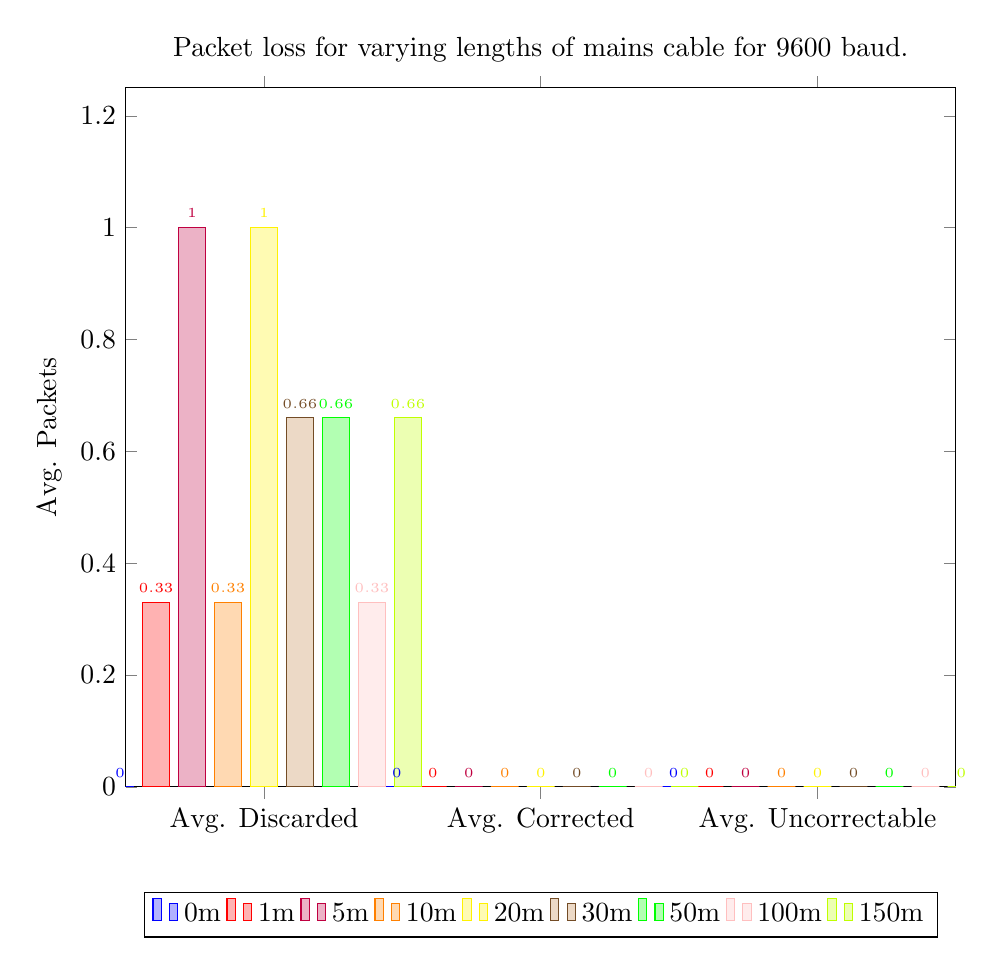
\begin{tikzpicture}
\begin{axis}[
    title=Packet loss for varying lengths of mains cable for 9600 baud.,
    ybar=3pt,
    ymin=0,
    width=\columnwidth,
    %cycle list name=bar cycle list,
    enlarge x limits=0.25,
    enlarge y limits={0.25,upper},
    legend style={at={(0.5,-0.15)},
      anchor=north,legend columns=-1},
    symbolic x coords={Avg. Discarded,Avg. Corrected,Avg. Uncorrectable},
    ylabel={Avg. Packets},
    xticklabel style={align=center},
	xtick=data,
    nodes near coords,
    every node near coord/.append style={font=\tiny},
    nodes near coords align={vertical},
]
%0
\addplot 
	coordinates {(Avg. Discarded,0)
		 (Avg. Corrected,0) (Avg. Uncorrectable,0)};
%1
\addplot 
	coordinates {(Avg. Discarded,0.33)
		 (Avg. Corrected,0) (Avg. Uncorrectable,0)};
%5
\addplot 
	coordinates {(Avg. Discarded,1)
		 (Avg. Corrected,0) (Avg. Uncorrectable,0)};
%10
\addplot 
	coordinates {(Avg. Discarded,0.33)
		 (Avg. Corrected,0) (Avg. Uncorrectable,0)};
%20
\addplot 
	coordinates {(Avg. Discarded,1)
		 (Avg. Corrected,0) (Avg. Uncorrectable,0)};
%30
\addplot 
	coordinates {(Avg. Discarded,0.66)
		 (Avg. Corrected,0) (Avg. Uncorrectable,0)};
%50
\addplot 
	coordinates {(Avg. Discarded,0.66)
		 (Avg. Corrected,0) (Avg. Uncorrectable,0)};
%100
\addplot 
	coordinates {(Avg. Discarded,0.33)
		 (Avg. Corrected,0) (Avg. Uncorrectable,0)};
%150
\addplot 
	coordinates {(Avg. Discarded,0.66)
		 (Avg. Corrected,0) (Avg. Uncorrectable,0)};
\legend{0m,1m,5m,10m,20m,30m,50m,100m,150m}
\end{axis}
\end{tikzpicture}
\caption{The results from the tests.}
\label{fig:pktlossmains}
\end{figure}
Figure~\ref{fig:pktlossmains} shows the average number of discarded packets, the average number of corrected packets and the average number of uncorrectable packets.\\
The graph shows that there isn't any correlation between distance and the average number of corrected, and uncorrectable packets. It also shows that there isn't a distinct correlation between discarded packets and cable length.\\
The experiment presented an unknown issue. The hardware cannot cope with a baud rate higher than 9600, as shown by the singular graph above. The same experiment was repeated on the previously identified baud rates, and the hub was unable to identify any clean packets.\\
The reason for this was due to the OpAmp which has a slew rate of 0.5 volts per microsecond. It deformed the packets received hub side, meaning that that could not be recognised by the Hub. The effect of the slew rate can be seen in the following image:
\begin{figure}[H]
    \centering
    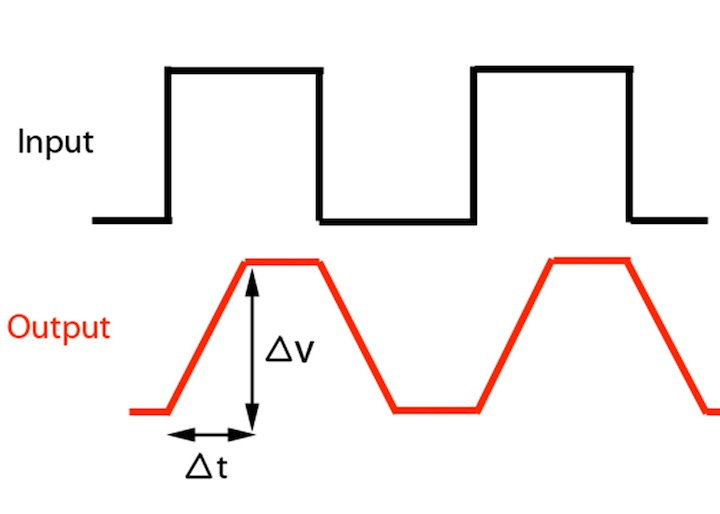
\includegraphics[width=6cm]{/tests/slew}
    \caption {A graphical representation of how the slew rate affects square waves~\cite{slew}}
\end{figure}

\subsubsection{Conclusions}
There is only one conclusion that can be drawn from the evaluation of the Fuse: The baud rate is low, and the selected OpAmp means that a faster baud rate cannot be used.\\
A different OpAmp with a lower slew rate could be used to improve the data rate in future so to ensure that the hub can correctly receive packets.


\subsection{Hub}
\subsubsection{Test Outline}
The next test to be performed concerned only the hub. This test was designed to assess the overall effectiveness of error detection and correction Hub-side.\\
The testing apparatus consisted of two Raspberry Pi's. One Pi would act as the fuse, and send a stream of packets to the Hub.\\ 
A whole new program was devised that generated packets, recorded each packet and it's type, and the time it was sent from the 'Fuse' Pi.\\
The packets sent from the 'Fuse' Pi consisted of some percentage of each type of packet: a correct packet, a correctable packet, an uncorrectable packet and a packet with an incorrect checksum. These packets were randomly ordered and streamed to the Pi.\\
The script used for testing the Fuse was used again to record the received packets, and each type the received packet had for the Hub.\\
The two data sets generated from the Hub and the 'Fuse' Pi could then be correlated and cross examined to produce statistics about the capture rate and the different detection rates of each type of packet.\\
Google Sheets was once again used to collate and analyse the data into a short summary that could be used to generate graphs.\\
Both programs logged the data in CSV format making it extremely easy to transform into a spreadsheet.
\subsubsection{Results}
Each graph shows the results generated from the test outlined in the previous section.\\
Each series label represents the number of each type of packet used in that test, it is formatted as follows:\\
\textit{Correct packets / Incorrect packets / Uncorrectable packets / Incorrect checksum packets}
\begin{figure}[H]
\centering
\resizebox {!} {10cm} {
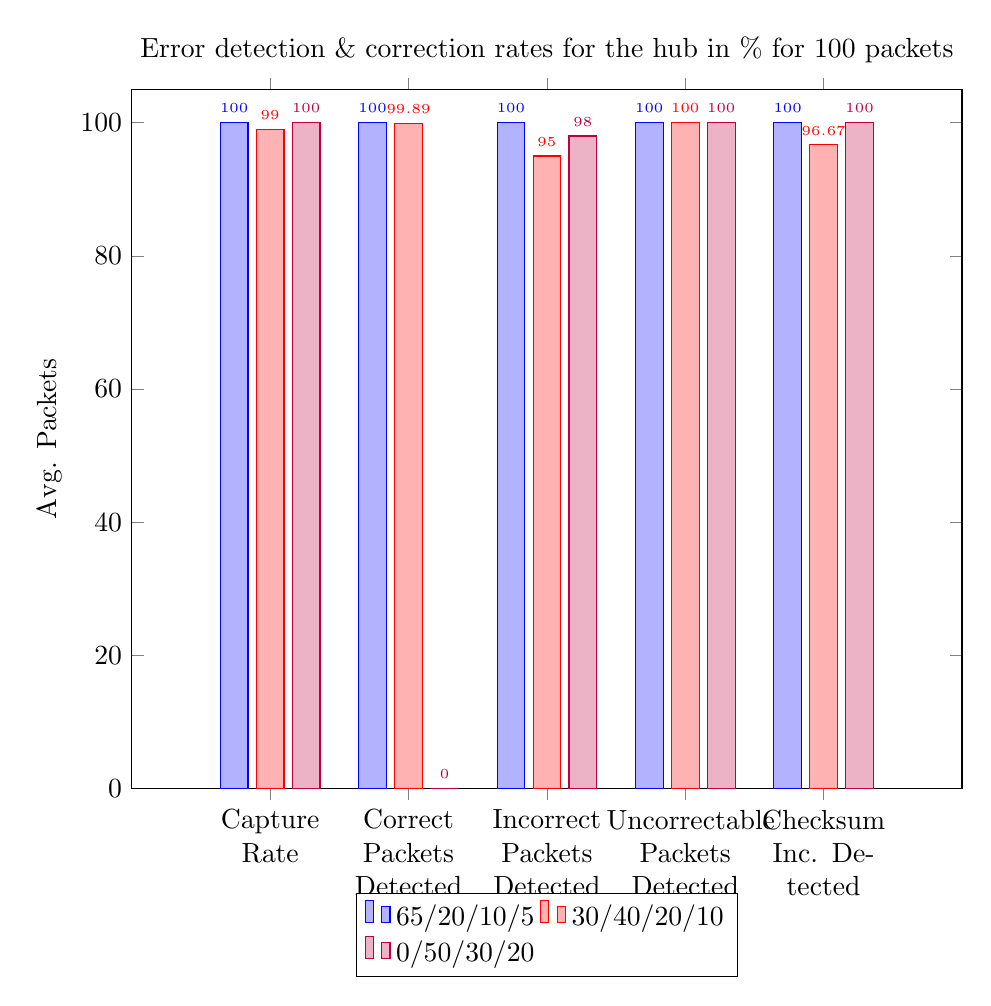
\begin{tikzpicture}
\begin{axis}[
    title=Error detection \& correction rates for the hub in \% for 100 packets,
    ybar=3pt,
    ymin=0,
    ymax=105,
    width=\columnwidth,
    %cycle list name=bar cycle list,
    enlarge x limits=0.25,
    legend columns=2,
    %enlarge y limits={0.25,upper},
    legend style={at={(0.5,-0.15)},
      anchor=north,legend columns=-1},
    symbolic x coords={Capture Rate,Correct Packets Detected,Incorrect Packets Detected,Uncorrectable Packets Detected, Checksum Inc. Detected},
    ylabel={Avg. Packets},
	xtick=data,
    nodes near coords,
    every node near coord/.append style={font=\tiny},
    nodes near coords align={vertical},
    xticklabel style={align=center,text width=2cm},
]
%100 65/20/10/5
\addplot 
	coordinates {(Capture Rate,100)
		 (Correct Packets Detected,100) (Incorrect Packets Detected,100)(Uncorrectable Packets Detected,100)(Checksum Inc. Detected,100)};
%100 30/40/20/10
\addplot 
	coordinates {(Capture Rate,99)
		 (Correct Packets Detected,99.89) (Incorrect Packets Detected,95)(Uncorrectable Packets Detected,100)(Checksum Inc. Detected,96.67)};
%100 0/50/30/20
\addplot 
	coordinates {(Capture Rate,100)
		 (Correct Packets Detected,0) (Incorrect Packets Detected,98)(Uncorrectable Packets Detected,100)(Checksum Inc. Detected,100)};

\legend{65/20/10/5,30/40/20/10,0/50/30/20}
\end{axis}
\end{tikzpicture}
}
\end{figure}


\begin{figure}[H]
\centering
\resizebox {!} {10cm} {
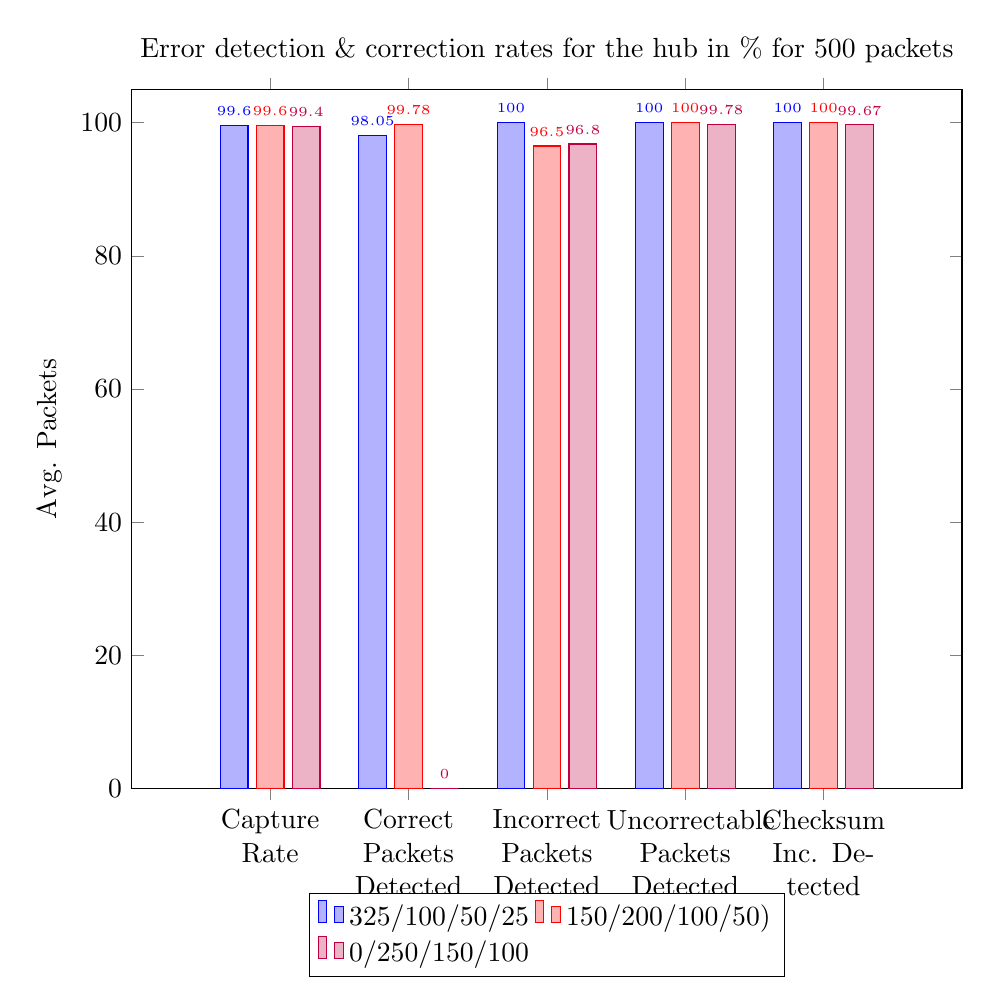
\begin{tikzpicture}
\begin{axis}[
    title=Error detection \& correction rates for the hub in \% for 500 packets,
    ybar=3pt,
    ymin=0,
    ymax=105,
    width=\columnwidth,
    %cycle list name=bar cycle list,
    enlarge x limits=0.25,
    legend columns=2,
    %enlarge y limits={0.25,upper},
    legend style={at={(0.5,-0.15)},
      anchor=north,legend columns=-1},
    symbolic x coords={Capture Rate,Correct Packets Detected,Incorrect Packets Detected,Uncorrectable Packets Detected, Checksum Inc. Detected},
    ylabel={Avg. Packets},
	xtick=data,
    nodes near coords,
    every node near coord/.append style={font=\tiny},
    nodes near coords align={vertical},
    xticklabel style={align=center,text width=2cm},
]

%500 65/20/10/5
\addplot 
	coordinates {(Capture Rate,99.6)
		 (Correct Packets Detected,98.05) (Incorrect Packets Detected,100)(Uncorrectable Packets Detected,100)(Checksum Inc. Detected,100)};
%500 30/40/20/10
\addplot 
	coordinates {(Capture Rate,99.6)
		 (Correct Packets Detected,99.78) (Incorrect Packets Detected,96.5)(Uncorrectable Packets Detected,100)(Checksum Inc. Detected,100)};
		 
%500 0/50/30/20
\addplot 
	coordinates {(Capture Rate,99.4)
		 (Correct Packets Detected,0) (Incorrect Packets Detected,96.8)(Uncorrectable Packets Detected,99.78)(Checksum Inc. Detected,99.67)};

\legend{325/100/50/25,150/200/100/50),0/250/150/100}
\end{axis}
\end{tikzpicture}
}
\end{figure}

\begin{figure}[H]
\centering
\resizebox {!} {10cm} {
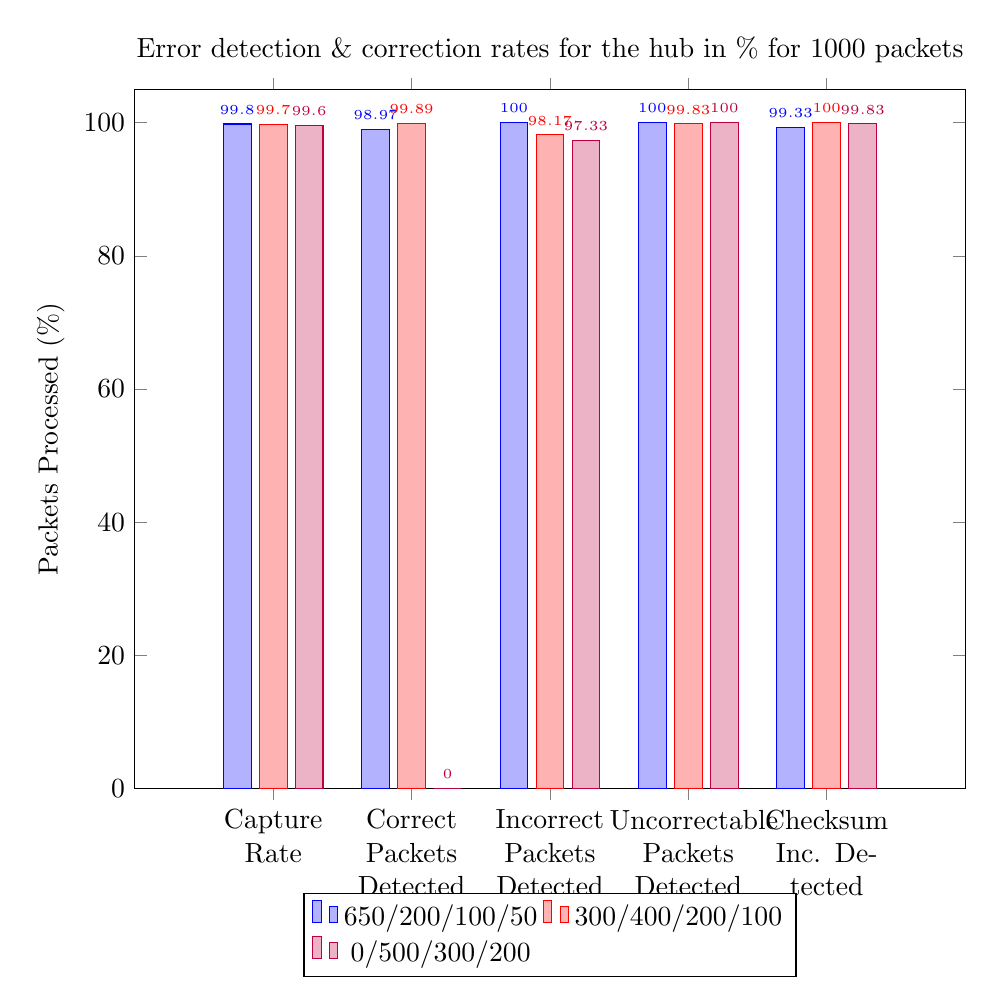
\begin{tikzpicture}
\begin{axis}[
    title=Error detection \& correction rates for the hub in \% for 1000 packets,
    ybar=3pt,
    ymin=0,
    ymax=105,
    width=\columnwidth,
    %cycle list name=bar cycle list,
    enlarge x limits=0.25,
    legend columns=2,
    %enlarge y limits={0.25,upper},
    legend style={at={(0.5,-0.15)},
      anchor=north,legend columns=-1},
    symbolic x coords={Capture Rate,Correct Packets Detected,Incorrect Packets Detected,Uncorrectable Packets Detected, Checksum Inc. Detected},
    ylabel={Packets Processed (\%)},
	xtick=data,
    nodes near coords,
    every node near coord/.append style={font=\tiny},
    nodes near coords align={vertical},
    xticklabel style={align=center,text width=2cm},
]
		 
%1000 65/20/10/5
\addplot 
	coordinates {(Capture Rate,99.8)
		 (Correct Packets Detected,98.97) (Incorrect Packets Detected,100)(Uncorrectable Packets Detected,100)(Checksum Inc. Detected,99.33)};
%1000 30/40/20/10
\addplot 
	coordinates {(Capture Rate,99.7)
		 (Correct Packets Detected,99.89) (Incorrect Packets Detected,98.17)(Uncorrectable Packets Detected,99.83)(Checksum Inc. Detected,100)};
%1000 0/50/30/20
\addplot 
	coordinates {(Capture Rate,99.6)
		 (Correct Packets Detected,0) (Incorrect Packets Detected,97.33)(Uncorrectable Packets Detected,100)(Checksum Inc. Detected,99.83)};

\legend{650/200/100/50,300/400/200/100,0/500/300/200}
\end{axis}
\end{tikzpicture}
}
\end{figure}
The graphs show that the overall error correction \& error detection rates for the hub are almost perfect.\\
In a few of the tests packets were discarded by the Hub. When a packet is discarded on the hub, there is a cool off period before resuming listening for the beginning of the next packet to the value of 1.5 milliseconds. Therefore, if one packet is lost, at the rate the 'Fuse' Pi was transmitting, 2 packets would be lost which is why there is a mismatch between the number of sent packets and received packets. 

\subsubsection{Conclusions}
Overall, the evaluation of the error correction and detection capabilities of the Hub has proved to be very successful. The Hub appears to be pretty impervious to errors, and it detected the 100\% of each type of packet that it received.\\
Once point to note however for possibly future improvement, is the cool off period between discarding a packet and resuming the next packet. Some fine tuning on this aspect could improve the capture rate of the hub.

\subsection{App}
\subsubsection{Test Cases}

The following tables are the test cases of the application for the project. Each test has a purpose, a distinct number of steps and a clear result.

%% REGISTER %%

\begin{tabularx}{\columnwidth}{| p{\dimexpr 0.2\columnwidth-2\tabcolsep} | p{ \dimexpr 0.1\columnwidth-2\tabcolsep} | p{\dimexpr 0.35\columnwidth-2\tabcolsep} | p{\dimexpr 0.35\columnwidth-2\tabcolsep} |}


\hline
\textbf{Case:} & \multicolumn{3}{ p{\dimexpr 0.8\columnwidth-2\tabcolsep} |}{\textbf{Register Functionality}} \\

\hline
\textbf{Purpose} & \multicolumn{3}{p{\dimexpr 0.8\columnwidth-2\tabcolsep} |}{To determine whether the in-app registration feature works correctly} \\

\hline
\multirow{3}{*}{\textbf{Criteria}} &
\multicolumn{2}{p{\dimexpr 0.35\columnwidth-2\tabcolsep} |}{\textbf{Test Step}} & \multicolumn{1}{p{\dimexpr 0.35\columnwidth-2\tabcolsep} |}{\textbf{Expected Results}}\\\cline{2-4}
    & No. & Description & Description\\\cline{2-4}
    & 1   & The user enters their name, their email address and their desired password and the user taps the Register button. & The details are sent to the server, and returned to the application, the user is then subsequently logged in providing details are correct.\\ 
\hline
\textbf{Actual \newline Result} & \multicolumn{3}{ p{\dimexpr 0.8\columnwidth-2\tabcolsep} |}{\textcolor{OliveGreen}{\textbf{SUCCESS}} - The new user was automatically logged in and redirected to the home screen.}\\
\hline
\end{tabularx}\\[5pt]

%% LOGIN %%

\begin{tabularx}{\columnwidth}{| p{\dimexpr 0.2\columnwidth-2\tabcolsep} | p{ \dimexpr 0.1\columnwidth-2\tabcolsep} | p{\dimexpr 0.35\columnwidth-2\tabcolsep} | p{\dimexpr 0.35\columnwidth-2\tabcolsep} |}


\hline
\textbf{Case:} & \multicolumn{3}{ p{\dimexpr 0.8\columnwidth-2\tabcolsep} |}{\textbf{Login Functionality}} \\

\hline
\textbf{Purpose} & \multicolumn{3}{p{\dimexpr 0.8\columnwidth-2\tabcolsep} |}{To determine whether an existing using can log in to the application} \\

\hline
\multirow{3}{*}{\textbf{Criteria}} &
\multicolumn{2}{p{\dimexpr 0.35\columnwidth-2\tabcolsep} |}{\textbf{Test Step}} & \multicolumn{1}{p{\dimexpr 0.35\columnwidth-2\tabcolsep} |}{\textbf{Expected Results}}\\\cline{2-4}
    & No. & Description & Description\\\cline{2-4}
    & 1    & The user enters their user name and password and taps the Login button. & The user should be redirected to the home screen upon a successful login with correct credentials.\\
\hline

\textbf{Actual \newline Result} & \multicolumn{3}{ p{\dimexpr 0.8\columnwidth-2\tabcolsep} |}{\textcolor{OliveGreen}{\textbf{SUCCESS}} -  The existing user was logged in, and redirected to the home screen}\\
\hline
\end{tabularx}\\[5pt]

%% FUSE DETAILS %%

\begin{tabularx}{\columnwidth}{| p{\dimexpr 0.2\columnwidth-2\tabcolsep} | p{ \dimexpr 0.1\columnwidth-2\tabcolsep} | p{\dimexpr 0.35\columnwidth-2\tabcolsep} | p{\dimexpr 0.35\columnwidth-2\tabcolsep} |}


\hline
\textbf{Case:} & \multicolumn{3}{ p{\dimexpr 0.8\columnwidth-2\tabcolsep} |}{\textbf{Updating Fuse Details Functionality}} \\

\hline
\textbf{Purpose} & \multicolumn{3}{p{\dimexpr 0.8\columnwidth-2\tabcolsep} |}{To determine whether a user can edit a fuse, and update the details stored on the server.} \\

\hline
\multirow{3}{*}{\textbf{Criteria}} &
\multicolumn{2}{p{\dimexpr 0.35\columnwidth-2\tabcolsep} |}{\textbf{Test Step}} & \multicolumn{1}{p{\dimexpr 0.35\columnwidth-2\tabcolsep} |}{\textbf{Expected Results}}\\\cline{2-4}
    & No. & Description & Description\\\cline{2-4}
    & 1    & The user taps on the desired fuses' edit button, amends the fuses' details as required and taps the Update button. & The updated fuse details are sent to the server, and synced back with the client, the modal then closes closes.\\
\hline

\textbf{Actual \newline Result} & \multicolumn{3}{ p{\dimexpr 0.8\columnwidth-2\tabcolsep} |}{\textcolor{OliveGreen}{\textbf{SUCCESS}} -  The user was able to adjust the Fuse details, and those changes were synced with the server.}\\
\hline
\end{tabularx}\\[5pt]

%% FUSE IMAGE UPLOAD %%

\begin{tabularx}{\columnwidth}{| p{\dimexpr 0.2\columnwidth-2\tabcolsep} | p{ \dimexpr 0.1\columnwidth-2\tabcolsep} | p{\dimexpr 0.35\columnwidth-2\tabcolsep} | p{\dimexpr 0.35\columnwidth-2\tabcolsep} |}


\hline
\textbf{Case:} & \multicolumn{3}{ p{\dimexpr 0.8\columnwidth-2\tabcolsep} |}{\textbf{Fuse Image Upload Functionality}} \\

\hline
\textbf{Purpose} & \multicolumn{3}{p{\dimexpr 0.8\columnwidth-2\tabcolsep} |}{To determine whether an existing user can update a fuse with a new profile picture.} \\

\hline
\multirow{3}{*}{\textbf{Criteria}} &
\multicolumn{2}{p{\dimexpr 0.35\columnwidth-2\tabcolsep} |}{\textbf{Test Step}} & \multicolumn{1}{p{\dimexpr 0.35\columnwidth-2\tabcolsep} |}{\textbf{Expected Results}}\\\cline{2-4}
    & No. & Description & Description\\\cline{2-4}
    & 1    & The user taps on the desired fuses edit button, taps the 'Upload new photo' button, takes a picture and hits ok.  & The new image is then uploaded to the server, and is synced with the client.\\
\hline

\textbf{Actual \newline Result} & \multicolumn{3}{ p{\dimexpr 0.8\columnwidth-2\tabcolsep} |}{\textcolor{red}{\textbf{FAIL}} -  Using a large phone (iPhone 6+) to take the photo caused the application to crash. \newline This was tested again on the iPhone 5, and it uploaded without a hitch.}\\
\hline
\end{tabularx}\\[5pt]

%% FUSE DELETE %%

\begin{tabularx}{\columnwidth}{| p{\dimexpr 0.2\columnwidth-2\tabcolsep} | p{ \dimexpr 0.1\columnwidth-2\tabcolsep} | p{\dimexpr 0.35\columnwidth-2\tabcolsep} | p{\dimexpr 0.35\columnwidth-2\tabcolsep} |}


\hline
\textbf{Case:} & \multicolumn{3}{ p{\dimexpr 0.8\columnwidth-2\tabcolsep} |}{\textbf{Delete a Fuse Functionality}} \\

\hline
\textbf{Purpose} & \multicolumn{3}{p{\dimexpr 0.8\columnwidth-2\tabcolsep} |}{To determine whether an existing user can remove a fuse from their accout.} \\

\hline
\multirow{3}{*}{\textbf{Criteria}} &
\multicolumn{2}{p{\dimexpr 0.35\columnwidth-2\tabcolsep} |}{\textbf{Test Step}} & \multicolumn{1}{p{\dimexpr 0.35\columnwidth-2\tabcolsep} |}{\textbf{Expected Results}}\\\cline{2-4}
    & No. & Description & Description\\\cline{2-4}
    & 1    & The user swipes left on the fuse they would like to delete and taps the delete button.  & The fuse is removed from the list of fuses and isn't shown again until the fuse next reports..\\
\hline

\textbf{Actual \newline Result} & \multicolumn{3}{ p{\dimexpr 0.8\columnwidth-2\tabcolsep} |}{\textcolor{OliveGreen}{\textbf{SUCCESS}} - The fuse was removed from the account, and then at the next time the fuse reported data, the fuse was added back to the list.}\\
\hline
\end{tabularx}\\[5pt]

%% FUSE LIVE DATA %%

\begin{tabularx}{\columnwidth}{| p{\dimexpr 0.2\columnwidth-2\tabcolsep} | p{ \dimexpr 0.1\columnwidth-2\tabcolsep} | p{\dimexpr 0.35\columnwidth-2\tabcolsep} | p{\dimexpr 0.35\columnwidth-2\tabcolsep} |}


\hline
\textbf{Case:} & \multicolumn{3}{ p{\dimexpr 0.8\columnwidth-2\tabcolsep} |}{\textbf{Live Data Functionality}} \\

\hline
\textbf{Purpose} & \multicolumn{3}{p{\dimexpr 0.8\columnwidth-2\tabcolsep} |}{To determine if a user can view live data reported by a fuse} \\

\hline
\multirow{3}{*}{\textbf{Criteria}} &
\multicolumn{2}{p{\dimexpr 0.35\columnwidth-2\tabcolsep} |}{\textbf{Test Step}} & \multicolumn{1}{p{\dimexpr 0.35\columnwidth-2\tabcolsep} |}{\textbf{Expected Results}}\\\cline{2-4}
    & No. & Description & Description\\\cline{2-4}
    & 1    & The user taps on a fuse and is presented with the live view. & The user is able to see live data being reported by the fuse.\\
\hline

\textbf{Actual \newline Result} & \multicolumn{3}{ p{\dimexpr 0.8\columnwidth-2\tabcolsep} |}{\textcolor{OliveGreen}{\textbf{SUCCESS}} -  The user could see live data being reported by the Fuse}\\
\hline
\end{tabularx}\\[5pt]

%% ADD HUB %%

\begin{tabularx}{\columnwidth}{| p{\dimexpr 0.2\columnwidth-2\tabcolsep} | p{ \dimexpr 0.1\columnwidth-2\tabcolsep} | p{\dimexpr 0.35\columnwidth-2\tabcolsep} | p{\dimexpr 0.35\columnwidth-2\tabcolsep} |}


\hline
\textbf{Case:} & \multicolumn{3}{ p{\dimexpr 0.8\columnwidth-2\tabcolsep} |}{\textbf{Add a Hub Functionality}} \\

\hline
\textbf{Purpose} & \multicolumn{3}{p{\dimexpr 0.8\columnwidth-2\tabcolsep} |}{To determine if a user can link their account with a hub} \\

\hline
\multirow{3}{*}{\textbf{Criteria}} &
\multicolumn{2}{p{\dimexpr 0.35\columnwidth-2\tabcolsep} |}{\textbf{Test Step}} & \multicolumn{1}{p{\dimexpr 0.35\columnwidth-2\tabcolsep} |}{\textbf{Expected Results}}\\\cline{2-4}
    & No. & Description & Description\\\cline{2-4}
    & 1    & The user taps the plus button and types in the Hub ID. & The user is successfully able to link their hub and see data being reported by the fuses connected to that hub.\\
\hline

\textbf{Actual \newline Result} & \multicolumn{3}{ p{\dimexpr 0.8\columnwidth-2\tabcolsep} |}{\textcolor{OliveGreen}{\textbf{SUCCESS}} -  After the user entered the new hub ID and linked it with their account, the fuses screen was updted, and allowed the viewing of the additional hub.}\\
\hline
\end{tabularx}\\[5pt]

%% REMOVE HUB %%

\begin{tabularx}{\columnwidth}{| p{\dimexpr 0.2\columnwidth-2\tabcolsep} | p{ \dimexpr 0.1\columnwidth-2\tabcolsep} | p{\dimexpr 0.35\columnwidth-2\tabcolsep} | p{\dimexpr 0.35\columnwidth-2\tabcolsep} |}


\hline
\textbf{Case:} & \multicolumn{3}{ p{\dimexpr 0.8\columnwidth-2\tabcolsep} |}{\textbf{Remove a Hub Functionality}} \\

\hline
\textbf{Purpose} & \multicolumn{3}{p{\dimexpr 0.8\columnwidth-2\tabcolsep} |}{To determine if a user can unlink their user account with a hub.} \\

\hline
\multirow{3}{*}{\textbf{Criteria}} &
\multicolumn{2}{p{\dimexpr 0.35\columnwidth-2\tabcolsep} |}{\textbf{Test Step}} & \multicolumn{1}{p{\dimexpr 0.35\columnwidth-2\tabcolsep} |}{\textbf{Expected Results}}\\\cline{2-4}
    & No. & Description & Description\\\cline{2-4}
    & 1    & The user swipes left on the desired hub, and taps the delete button & The hub should is unlinked with the user account.\\
\hline

\textbf{Actual \newline Result} & \multicolumn{3}{ p{\dimexpr 0.8\columnwidth-2\tabcolsep} |}{\textcolor{OliveGreen}{\textbf{SUCCESS}} -  After the user tapped the delete button, the hub was then unlinked from the user account, and no fuses were displayed.}\\
\hline
\end{tabularx}\\[5pt]

%% Carbon Statistics %%

\begin{tabularx}{\columnwidth}{| p{\dimexpr 0.2\columnwidth-2\tabcolsep} | p{ \dimexpr 0.1\columnwidth-2\tabcolsep} | p{\dimexpr 0.35\columnwidth-2\tabcolsep} | p{\dimexpr 0.35\columnwidth-2\tabcolsep} |}


\hline
\textbf{Case:} & \multicolumn{3}{ p{\dimexpr 0.8\columnwidth-2\tabcolsep} |}{\textbf{Carbon Statistics Functionality}} \\

\hline
\textbf{Purpose} & \multicolumn{3}{p{\dimexpr 0.8\columnwidth-2\tabcolsep} |}{To determine if a user can view the current Carbon statistics for the UK.} \\

\hline
\multirow{3}{*}{\textbf{Criteria}} &
\multicolumn{2}{p{\dimexpr 0.35\columnwidth-2\tabcolsep} |}{\textbf{Test Step}} & \multicolumn{1}{p{\dimexpr 0.35\columnwidth-2\tabcolsep} |}{\textbf{Expected Results}}\\\cline{2-4}
    & No. & Description & Description\\\cline{2-4}
    & 1    & The user taps on the Carbon statistics tab & The Carbon statistics should be displayed.\\
\hline

\textbf{Actual \newline Result} & \multicolumn{3}{ p{\dimexpr 0.8\columnwidth-2\tabcolsep} |}{\textcolor{OliveGreen}{\textbf{SUCCESS}} -  After the user tapped the Carbon statistics tab, the statistics were displayed.}\\
\hline
\end{tabularx}\\[5pt]

%% POWER Statistics %%

\begin{tabularx}{\columnwidth}{| p{\dimexpr 0.2\columnwidth-2\tabcolsep} | p{ \dimexpr 0.1\columnwidth-2\tabcolsep} | p{\dimexpr 0.35\columnwidth-2\tabcolsep} | p{\dimexpr 0.35\columnwidth-2\tabcolsep} |}


\hline
\textbf{Case:} & \multicolumn{3}{ p{\dimexpr 0.8\columnwidth-2\tabcolsep} |}{\textbf{Power Statistics Functionality}} \\

\hline
\textbf{Purpose} & \multicolumn{3}{p{\dimexpr 0.8\columnwidth-2\tabcolsep} |}{To determine if a user can view the current Power statistics for the UK.} \\

\hline
\multirow{3}{*}{\textbf{Criteria}} &
\multicolumn{2}{p{\dimexpr 0.35\columnwidth-2\tabcolsep} |}{\textbf{Test Step}} & \multicolumn{1}{p{\dimexpr 0.35\columnwidth-2\tabcolsep} |}{\textbf{Expected Results}}\\\cline{2-4}
    & No. & Description & Description\\\cline{2-4}
    & 1    & The user taps on the Power statistics tab & The Power statistics should be displayed.\\
\hline

\textbf{Actual \newline Result} & \multicolumn{3}{ p{\dimexpr 0.8\columnwidth-2\tabcolsep} |}{\textcolor{OliveGreen}{\textbf{SUCCESS}} -  After the user tapped the Power statistics tab, the statistics were displayed.}\\
\hline
\end{tabularx}\\[5pt]

%% Price Statistics %%

\begin{tabularx}{\columnwidth}{| p{\dimexpr 0.2\columnwidth-2\tabcolsep} | p{ \dimexpr 0.1\columnwidth-2\tabcolsep} | p{\dimexpr 0.35\columnwidth-2\tabcolsep} | p{\dimexpr 0.35\columnwidth-2\tabcolsep} |}


\hline
\textbf{Case:} & \multicolumn{3}{ p{\dimexpr 0.8\columnwidth-2\tabcolsep} |}{\textbf{Power Statistics Functionality}} \\

\hline
\textbf{Purpose} & \multicolumn{3}{p{\dimexpr 0.8\columnwidth-2\tabcolsep} |}{To determine if a user can view the current Price statistics for the UK.} \\

\hline
\multirow{3}{*}{\textbf{Criteria}} &
\multicolumn{2}{p{\dimexpr 0.35\columnwidth-2\tabcolsep} |}{\textbf{Test Step}} & \multicolumn{1}{p{\dimexpr 0.35\columnwidth-2\tabcolsep} |}{\textbf{Expected Results}}\\\cline{2-4}
    & No. & Description & Description\\\cline{2-4}
    & 1    & The user taps on the Price statistics tab & The Price statistics should be displayed.\\
\hline

\textbf{Actual \newline Result} & \multicolumn{3}{ p{\dimexpr 0.8\columnwidth-2\tabcolsep} |}{\textcolor{OliveGreen}{\textbf{SUCCESS}} -  After the user tapped the Price statistics tab, the statistics were displayed.}\\
\hline
\end{tabularx}\\[5pt]

%% Edit Profile %%

\begin{tabularx}{\columnwidth}{| p{\dimexpr 0.2\columnwidth-2\tabcolsep} | p{ \dimexpr 0.1\columnwidth-2\tabcolsep} | p{\dimexpr 0.35\columnwidth-2\tabcolsep} | p{\dimexpr 0.35\columnwidth-2\tabcolsep} |}


\hline
\textbf{Case:} & \multicolumn{3}{ p{\dimexpr 0.8\columnwidth-2\tabcolsep} |}{\textbf{Edit Profile Functionality}} \\

\hline
\textbf{Purpose} & \multicolumn{3}{p{\dimexpr 0.8\columnwidth-2\tabcolsep} |}{To determine if a user view and edit their profile.} \\

\hline
\multirow{3}{*}{\textbf{Criteria}} &
\multicolumn{2}{p{\dimexpr 0.35\columnwidth-2\tabcolsep} |}{\textbf{Test Step}} & \multicolumn{1}{p{\dimexpr 0.35\columnwidth-2\tabcolsep} |}{\textbf{Expected Results}}\\\cline{2-4}
    & No. & Description & Description\\\cline{2-4}
    & 1    & The user taps on profile item, changes some information, and taps the update button. & The Users' profile information should be synced with the server, and then updated on the client..\\
\hline

\textbf{Actual \newline Result} & \multicolumn{3}{ p{\dimexpr 0.8\columnwidth-2\tabcolsep} |}{\textcolor{OliveGreen}{\textbf{SUCCESS}} -  After the user tapped update, the user details were synced with the server and updated client side.}\\
\hline
\end{tabularx}\\[5pt]



\subsubsection{Proposed Usability Study}

Given more time, a full Usability study would be conducted with the aim of evaluating the usefulness of the application, and a study into how it affects user behaviour.\\
At the end of the usability study, each participant should answer the following questions:
\begin{itemize}
\item On a scale of 1-10, how easy is it to login or register using the application?
\item On a scale of 1-10, how easy is the application to Navigate?
\item On a scale of 1-10, how useful was the Home screen for the application?
\item On a scale of 1-10, how useful was the live data offered by the application?
\item On a scale of 1-10, how insightful were the live statistics offered by the application?
\item On a scale of 1-10, how would you rate the applications usefulness?
\item Do you feel that the application helped to lower the energy expenditure of your household? If so, how?
\item Do you feel that the application affected the times at which you used your big appliances? If not, why?
\item Any additional comments?
\end{itemize}
The results obtained from the usability study, would help narrow the scope of future work.

\subsubsection{Conclusions}
The majority of test cases resulted in successes, the one exception being a fault with the PhoneGap Cordova Camera plugin, when testing Image upload. The iPhone 6+ is a relatively new device, with a high number of pixels per inch, meaning that the image produced is too big for the Camera plugin to handle, causing it to crash.\\
A possible fix for this is to reduce the resolution of the image, or decrease the image size specifically for the iPhone 6+.\\
The proposed Usability Study would provide a number of insights into the project, that could help direct the future work for this project.


\subsection{Server}

\subsubsection{Test Outline}
To test the Server, a test was devised to perform various stress tests and see how the server reacts under various loads.\\
The server specification is as follows: a 2.3Ghz CPU and 4 gigabytes of RAM.\\
The stress tests were conducted using a piece of software called JMeter~\cite{jmeter}. This piece of software runs locally on a personal machine, and imitates a user specified number of clients. JMeter can generate a number of statistics and graphs, the main statistic this test was interested in was Concurrent Users Vs. Response Time.\\
To test the server, a single URL was called 100 times by X number of concurrent users, with a ramp up period of 10 seconds.\\
The maximum number of users that JMeter can support is 2200, therefore there were three test steps: 100, 1000 and 2000.\\
The selected URL was the Login url (\url{scc-devine.lancs.ac.uk:8000/api/user}) which returns quite a large JSON object (316 bytes), which has to be retrieved from the database. The tests used valid credentials which meant that the server had to fetch the data every request.

\subsubsection{Results}
In the following graphs, Users are referred to as Threads, because in JMeter a thread acts as a user.
\begin{figure}[H]
    \centering
    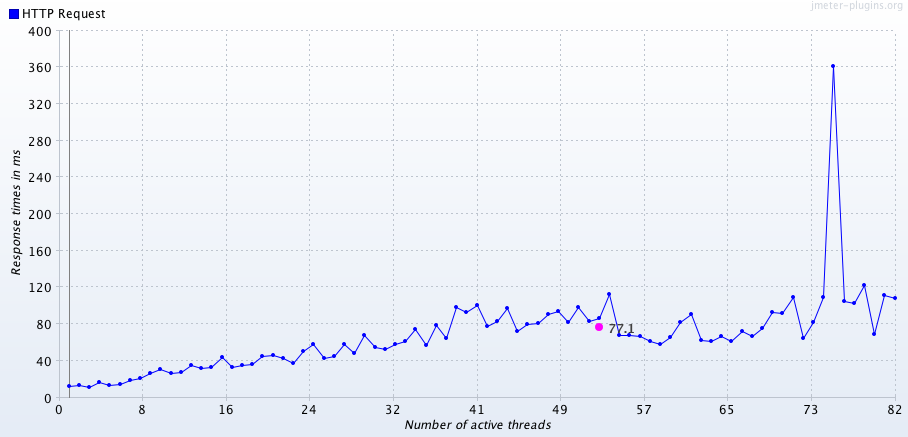
\includegraphics[width=\columnwidth]{/stresstests/users100}
    \caption {A stress test of 100 concurrent users performing 100 requests}
    \label{fig:stress100}
\end{figure}
Figure~\ref{fig:stress100} shows the results of a test of 100 concurrent users. The test shows that the server handles 100 concurrent clients pretty well with one bad spike where a user had to wait 400 ms for a response, which immediately scales back down for the next request.
\begin{figure}[H]
    \centering
    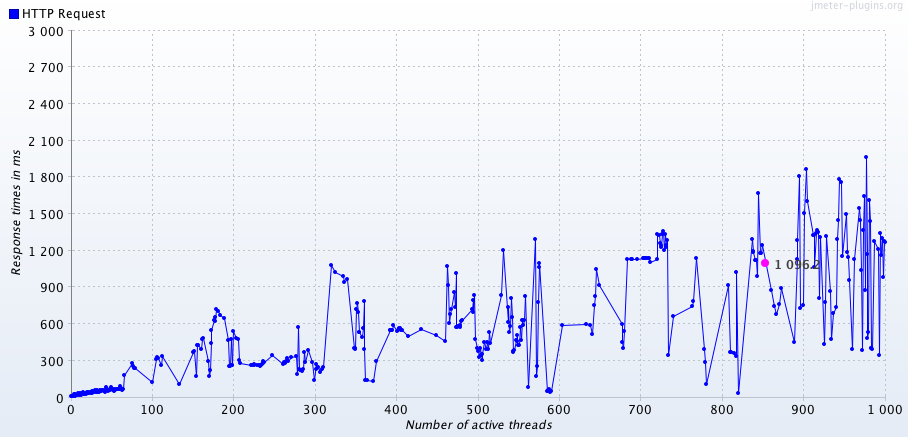
\includegraphics[width=\columnwidth]{/stresstests/users1000}
    \caption {A stress test of 1000 concurrent users performing 100 requests}
    \label{fig:stress1000}
\end{figure}
Figure~\ref{fig:stress1000} shows the results of a test of 1000 concurrent users. The Server starts well, with a steady increase of response time. As the number of users increases to 500 the difference in response times is huge, with a lot of random spikes. At 1000, the spikes are even worse with a peak of around 2000 ms response time.
\begin{figure}[H]
    \centering
    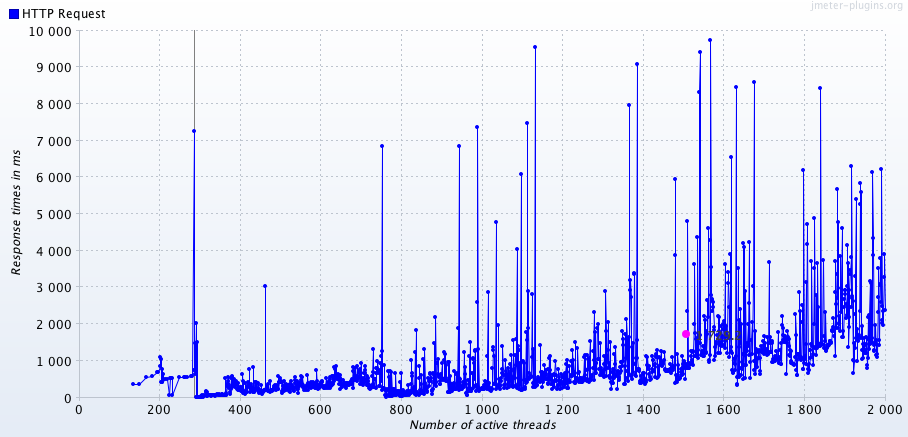
\includegraphics[width=\columnwidth]{/stresstests/users2000}
    \caption {A stress test of 2000 concurrent users performing 100 requests}
    \label{fig:stress2000}
\end{figure}
Figure~\ref{fig:stress1000} shows the results of a test of 2000 concurrent users. The server copes well to begin with, and at around 300 active users, there is a huge spike in response time, which immediately settles. Later, the huge variance in response time returns and becomes more sporadic the more concurrent users there are. The longest response time in this figure is around 9700 ms.

\begin{figure}[H]
    \centering
    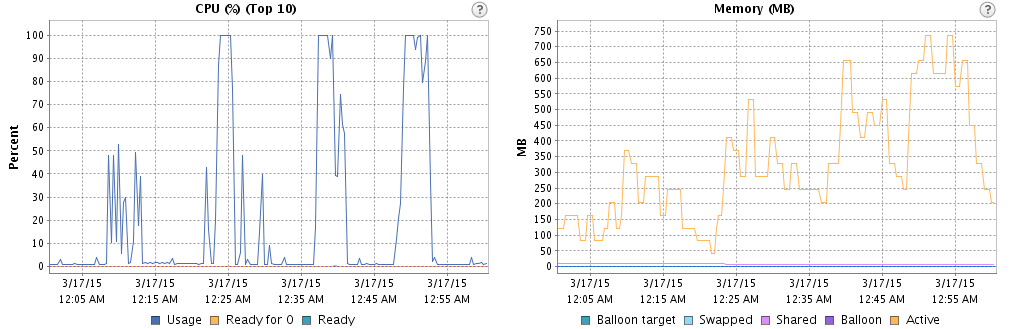
\includegraphics[width=\columnwidth]{/stresstests/vmware}
    \caption {The performance of the server as indicated by VMWare performance tools.}
    \label{fig:stressvmware}
\end{figure}
Figure~\ref{fig:stressvmware} shows the VMWare statistics. There are four clear spikes, the first being 100 concurrent users, the second 1000 concurrent users, the third 2000 concurrent users and the last one is an attempt at 10,000 users which was omitted.\\
Spikes can be seen in both the CPU graph and the Memory usage graph, and they clearly match onto one another. Interestingly, even though the CPU usage sky rockets, the memory usage remains pretty low in comparison.

\subsubsection{Conclusions}
It is clear from the stress tests that a single CPU server with a small amount of RAM is not up for the task of a hugely utilised system. However, the server-side software has been designed with this in mind, and is scalable across server clusters, allowing for a more robust, distributed system.

\section{Conclusions \& Future Work}

\clearpage
\bibliographystyle{plain}
\bibliography{master}{}

\end{document}
%
% ****** End of file apssamp.tex ******
